%%%%%%%%%%%%%%%%%%%%%%%%%%%%%%%%%%%%%%%%%
% Stylish Article
% LaTeX Template
% Version 2.1 (1/10/15)
%
% This template has been downloaded from:
% http://www.LaTeXTemplates.com
%
% Original author:
% Mathias Legrand (legrand.mathias@gmail.com) 
% With extensive modifications by:
% Vel (vel@latextemplates.com)
%
% License:
% CC BY-NC-SA 3.0 (http://creativecommons.org/licenses/by-nc-sa/3.0/)
%
%%%%%%%%%%%%%%%%%%%%%%%%%%%%%%%%%%%%%%%%%

%----------------------------------------------------------------------------------------
%	PACKAGES AND OTHER DOCUMENT CONFIGURATIONS
%----------------------------------------------------------------------------------------

\documentclass[fleqn,10pt]{SelfArx} % Document font size and equations flushed left

\usepackage{subcaption}
\usepackage[english]{babel} % Specify a different language here - english by default
\usepackage{array,booktabs}% http://ctan.org/pkg/{array,booktabs}
\usepackage{lipsum} % Required to insert dummy text. To be removed otherwise
\usepackage[section]{placeins}
\usepackage{amsmath}
\usepackage{longtable}
\newcolumntype{P}[1]{>{\centering\arraybackslash}p{#1}}
\newcolumntype{M}[1]{>{\centering\arraybackslash}m{#1}}
%----------------------------------------------------------------------------------------
%	COLUMNS
%----------------------------------------------------------------------------------------

\setlength{\columnsep}{0.55cm} % Distance between the two columns of text
\setlength{\fboxrule}{0.75pt} % Width of the border around the abstract

%----------------------------------------------------------------------------------------
%	COLORS
%----------------------------------------------------------------------------------------

\definecolor{color1}{RGB}{0,0,90} % Color of the article title and sections
\definecolor{color2}{RGB}{0,20,20} % Color of the boxes behind the abstract and headings

%----------------------------------------------------------------------------------------
%	HYPERLINKS
%----------------------------------------------------------------------------------------

\usepackage{hyperref} % Required for hyperlinks
\hypersetup{hidelinks,colorlinks,breaklinks=true,urlcolor=color2,citecolor=color1,linkcolor=color1,bookmarksopen=false,pdftitle={Title},pdfauthor={Author}}

%----------------------------------------------------------------------------------------
%	ARTICLE INFORMATION
%----------------------------------------------------------------------------------------

\JournalInfo{\today} % Journal information
\Archive{} % Additional notes (e.g. copyright, DOI, review/research article)

\PaperTitle{{\small ESE650 Project 5:} \\Cost Learning and Path Planning} % Article title

\Authors{Nischal K N\\nischal@seas.upenn.edu} % Authors
%\affiliation{\textsuperscript{1}\textit{Department of Biology, University of Examples, London, United Kingdom}} % Author affiliation
%\affiliation{\textsuperscript{2}\textit{Department of Chemistry, University of Examples, London, United Kingdom}} % Author affiliation
%\affiliation{*\textbf{Corresponding author}: john@smith.com} % Corresponding author

\Keywords{} % Keywords - if you don't want any simply remove all the text between the curly brackets
\newcommand{\keywordname}{Keywords} % Defines the keywords heading name

%----------------------------------------------------------------------------------------
%	ABSTRACT
%----------------------------------------------------------------------------------------

\Abstract{Imitation learning is an advanced behavior to replicate the previously supervised action. This is accomplished by learning the parameters of the model through the various supervised examples. In this project we learn the cost of various features of a satellite map through hand labeled routes to build a cost map for driving and walking. This is accomplished using gradient decent to choose the weights for each feature set.}

%----------------------------------------------------------------------------------------

\begin{document}

\flushbottom % Makes all text pages the same height

\maketitle % Print the title and abstract box

\tableofcontents % Print the contents section

\thispagestyle{empty} % Removes page numbering from the first page

%----------------------------------------------------------------------------------------
%	ARTICLE CONTENTS
%----------------------------------------------------------------------------------------
\section{Introduction}
In this project, the aim is to generate routes between any two points in a satellite image of penn campus. It has to support 2 modes, walking and driving. To accomplish this, we first hand label viable routes for both the modes. Based on the hand labeled paths weights we learn different cost maps for each mode. The cost map is a linear combination of weights multiplied to the feature map which are derived from the satellite image. The objective is to learn the weights of each feature map that minimizes the difference in the Dijkstra path and hand labeled path. This is achieved through gradient decent.

\section{Algorithm}
\label{sec:algo}
\begin{figure*}
    \centering
    \begin{subfigure}[t]{0.5\textwidth}
        \centering
        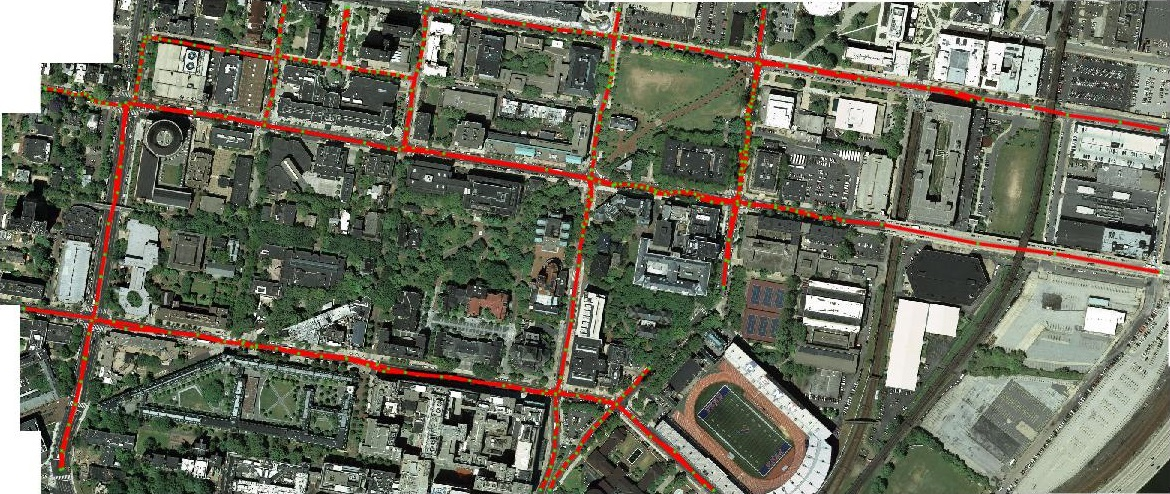
\includegraphics[scale = 0.3]{ex_car.jpg}
        \caption{Hand Labeled Drive paths}
        \label{fig:ex_car}
    \end{subfigure}%
    ~ 
    \begin{subfigure}[t]{0.5\textwidth}
        \centering
        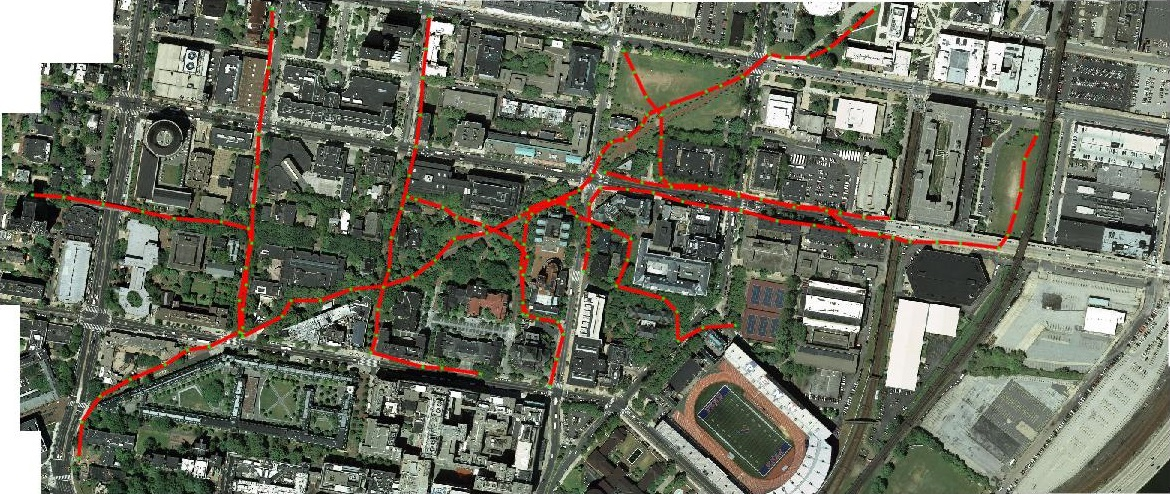
\includegraphics[scale = 0.3]{ex_walk.jpg}
        \caption{Hand Labeled Walk paths}
        \label{fig:ex_walk}
    \end{subfigure}
    \caption{Hand labeled paths}
    \label{fig:gr}
\end{figure*}

\subsection{Hand Labeling}
A number of paths are hand labeled using the ginput matlab function. GetMapCellsFromRay function is used to obtain the path between the clicked points from the ginput. Fig. \ref{fig:ex_car} and Fig. \ref{fig:ex_walk} shows the hand labeled paths for driving and walking modes respectively.

\subsection{Features}
A total of 24 features were used as the feature set. It included 16 Kmeans cluster in RGB color space with each cluster as a feature set and a unique feature map for unique objects such as white roof tops, black roof tops, tree cover, foot paths, etc either in HSV, YCbCr or Lab color space depending on which can capture the features better. They were manually picked using the color thresholder app in Matlab. 

Additionally to each of these feature maps, morphological operations were performed to reduce the effect of stray pixels. The series of morphological operations were
\begin{enumerate}
\itemsep-0.2em 
\item \textbf{spur} using bwmorph
\item \textbf{clean} using bw morph
\item \textbf{erode} using imerode with a disk structural element of size 2.
\item \textbf{dilate} using imdilate with a disk structural element of size 2.
\end{enumerate}

In few cases such as gray and black roof tops, quite a few roads were also present in the feature map. To remove these, the property of eccentricity was used. First the connected components are found out. Then for each of these connected components the area and eccentricity was thresholded. Anything above the threshold was consider as a road and hence removed as roads are more elongated and hence have higher eccentricity. Hence this preserved rooftops only.

To all the binary images, a Gaussian blur was applied. The list of features used and the operations performed on them are shown in Table \ref{tab:features}.

\subsection{Gradient Descent}
The following steps were performed to determine the weights of the feature maps
\begin{enumerate}
\item Weights $w$ were initialized uniformly and the cost map $C(x,y)$ was calculated using
\begin{align*}
w_i =&\; 1, \quad \forall i \\
C(x,y) =&\; e^{\sum_i w_i F_i(x,y)}
\end{align*}
Where $F_i(x,y)$ is the feature map and $i$ is the feature.
\item For each pair of training start and end points, Dijkstra path was created using the previously computed cost map $C(x,y)$. The path generated be $(x',y')$.
\item The gradient or the difference between hand labeled and Dijkstra map is calculated for each feature and the sum over each sample path is taken. Gradient is calculated as
\begin{align*}
\hspace{-1cm}
\frac{\delta J}{\delta w_i} =&\; \sum_{(x,y)} F_i(x,y) e^{\sum_i w_i F_i(x,y)} - \sum_{(x',y')} F_i(x',y') e^{\sum_i w_i F_i(x',y')} \\
\hspace{-1cm}
\frac{\delta J}{\delta w_i} =&\; \sum_{(x,y)} F_i(x,y) C(x,y) - \sum_{(x',y')} F_i(x',y') C(x',y') 
\end{align*}
Where $(x,y)$ are hand labeled paths and $(x',y')$ are Dijkstra generated paths.
\item The weights are updated using this gradient
\begin{align*}
w_i = w_i - \eta \frac{\delta J}{\delta w_i}
\end{align*}
Where $\eta$ is the learning rate.
\item The new cost map is calculated using the equation in step 1.
\item The termination condition is determined based on the difference between the costs of hand labeled path and Dijkstra path.
\begin{align*}
J = \sum_{(x,y)} C(x,y) - \sum_{(x',y')} C(x',y')
\end{align*}
If the difference is less than the threshold, the process is terminated, else its repeated from step 2.
\end{enumerate}
The final weights after convergence is shown in Table \ref{tab:weights} for both driving and walking.

\section{Experiments and Results}
\label{sec:results}
The cost map learned from the above process are shown in Fig. \ref{fig:costCar} for driving and Fig. \ref{fig:costWalk} for walking. The performance on test points is shown in Fig. \ref{fig:drive} for driving and Fig. \ref{fig:walk} for walking.      

\begin{table}
\caption{Weights for feature map}
\label{tab:weights}
\centering
\begin{tabular}{ccc}
\toprule
Feature & Driving Weights & Walking Weights \\ 
\midrule
K-means, K = 1 & -0.4807 & 0.7781 \\ 
\midrule
K-means, K = 2 & 0.0900 & 0.9951 \\ 
\midrule
K-means, K = 3 & -0.1071 & 0.8336 \\ 
\midrule
K-means, K = 4 & -1.0135 & 0.8306 \\ 
\midrule
K-means, K = 5 & -0.8823 & 0.8794 \\ 
\midrule
K-means, K = 6 & -0.0458 & 0.8255 \\ 
\midrule
K-means, K = 7 & 0.3423 & 0.9021 \\ 
\midrule
K-means, K = 8 & 0.2456 & 0.9357 \\ 
\midrule
K-means, K = 9 & -0.8598 & 0.8122 \\ 
\midrule
K-means, K = 10 & 0.6176 & 0.7909 \\ 
\midrule
K-means, K = 11 & 0.5919 & 0.8376 \\ 
\midrule
K-means, K = 12 & -0.9072 & 0.8991 \\ 
\midrule
K-means, K = 13 & -0.9023 & 0.7589 \\ 
\midrule
K-means, K = 14 & -0.9404 & 0.6724 \\ 
\midrule
K-means, K = 15 & -0.9351 & 0.7738 \\ 
\midrule
K-means, K = 16 & 0.8765 & 0.9710 \\ 
\midrule
Black roof & -0.8460 & 0.8327 \\ 
\midrule
Brown roof & -0.1785 & 0.5296 \\ 
\midrule
Grey roof & -0.3161 & 0.7979 \\ 
\midrule
Green trees & 1.0849 & 0.0357 \\ 
\midrule
Dark Grey & -0.0882 & 0.7150 \\ 
\midrule
White roof & 0.6745 & 0.9744 \\ 
\midrule
Cream roof & 0.9684 & 0.5953 \\ 
\midrule
roads & -1.1784 & -0.6059 \\ 
\bottomrule
\end{tabular} 
\end{table}

\begin{table*}
\caption{Features}
\label{tab:features}
\centering
\begin{tabular}{>{\centering\arraybackslash}M{8mm}cc>{\centering\arraybackslash}M{20mm}}
\toprule
Feature & Masked RGB Image & Feature & Post Processing \\ 
\midrule 
\vspace{-3cm}
\hspace{-0.6cm}
K-means, K = 1 & 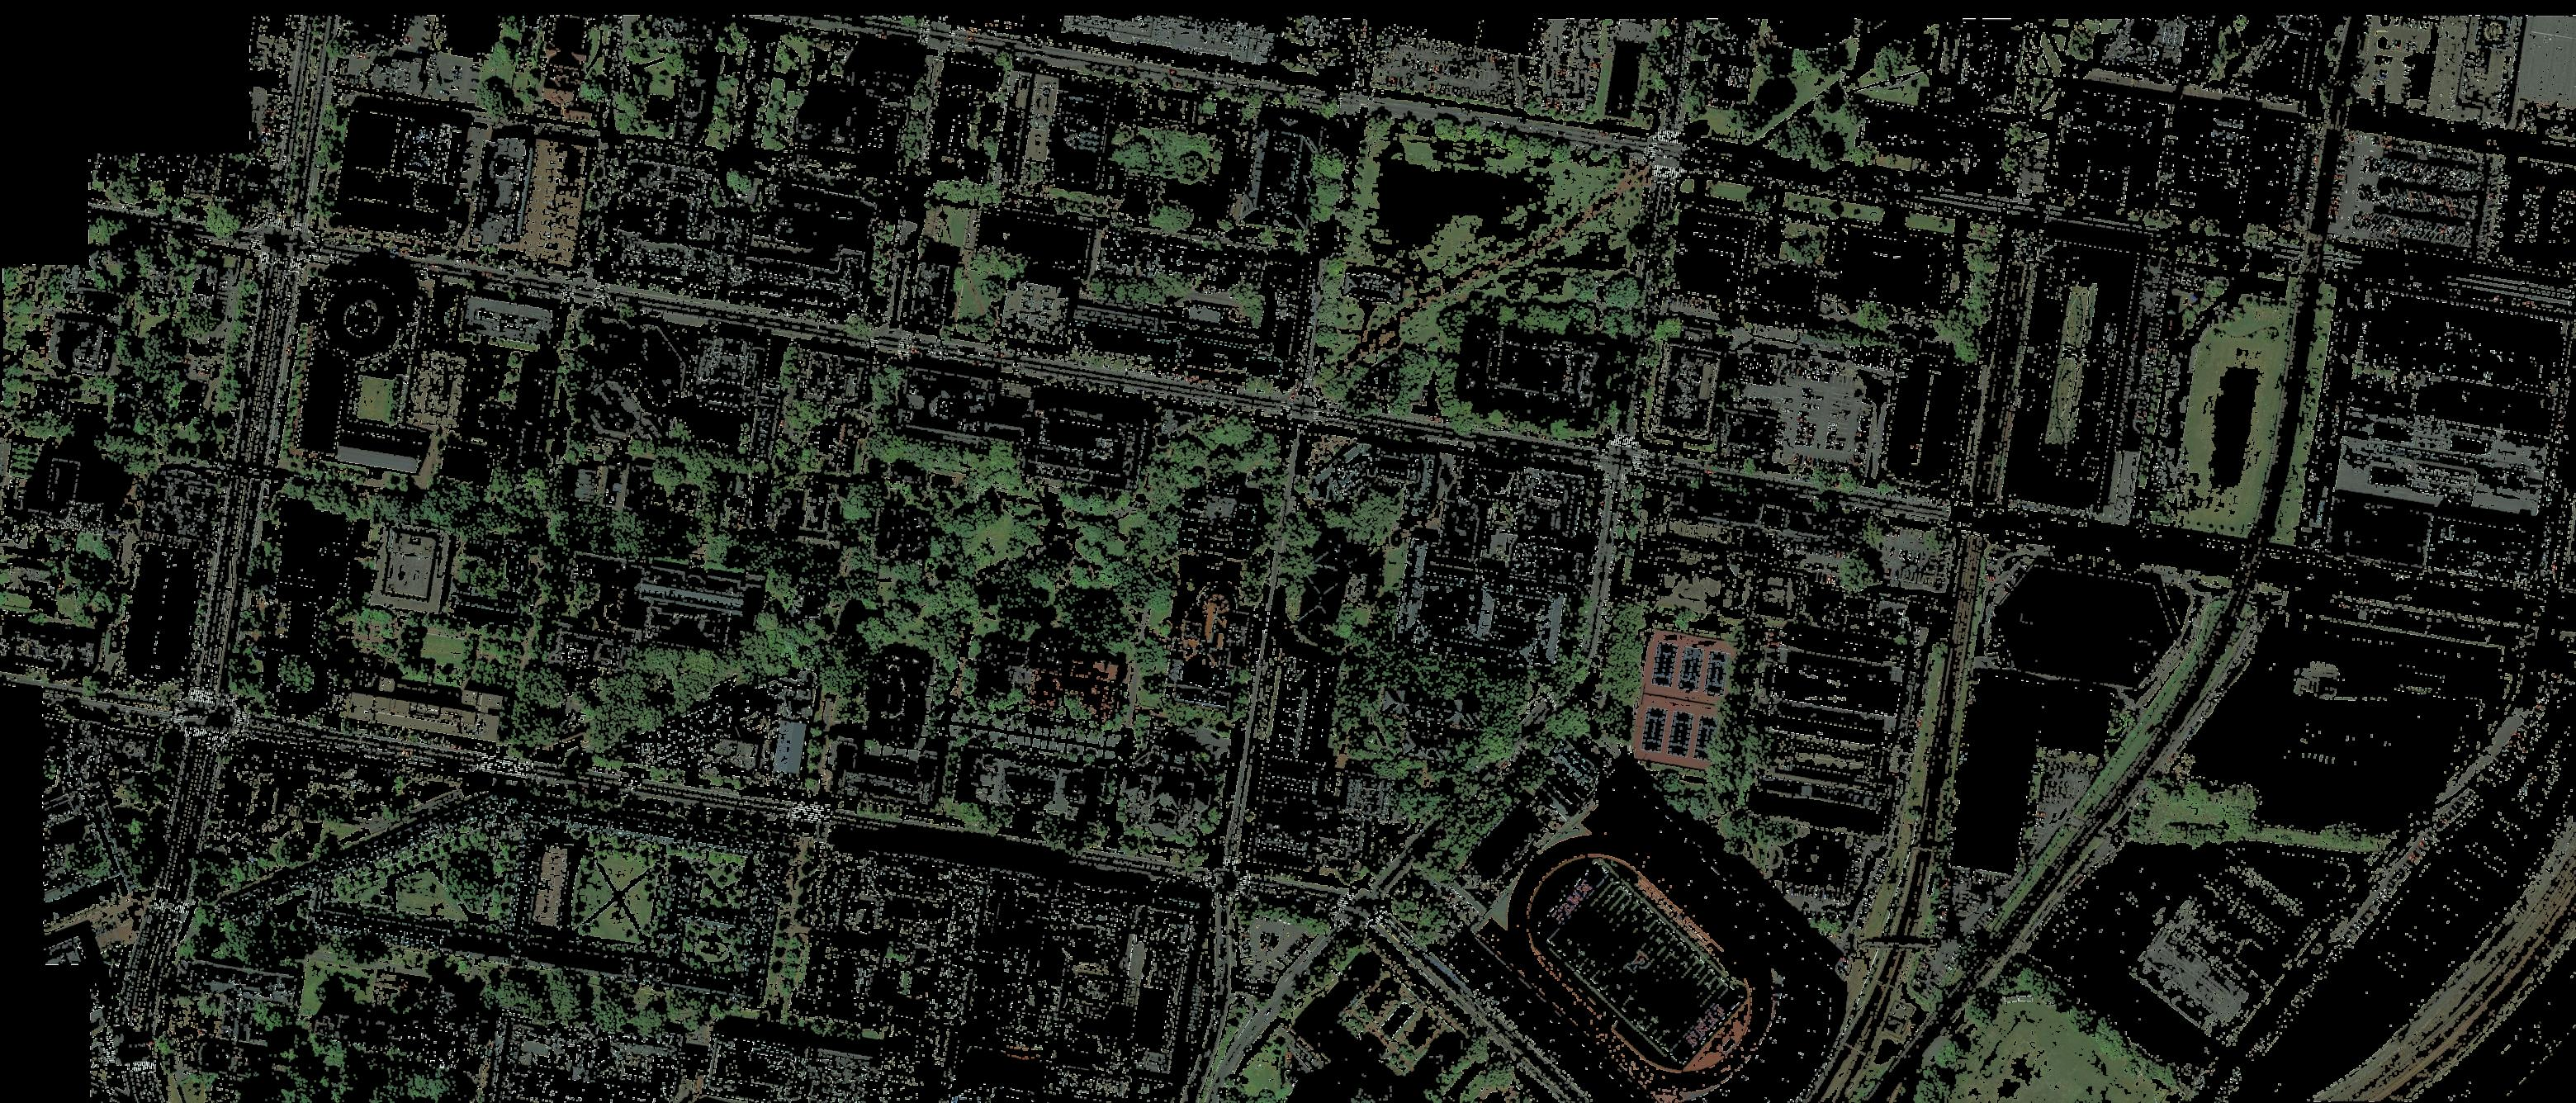
\includegraphics[clip,scale=0.07]{1rgb.jpg} & 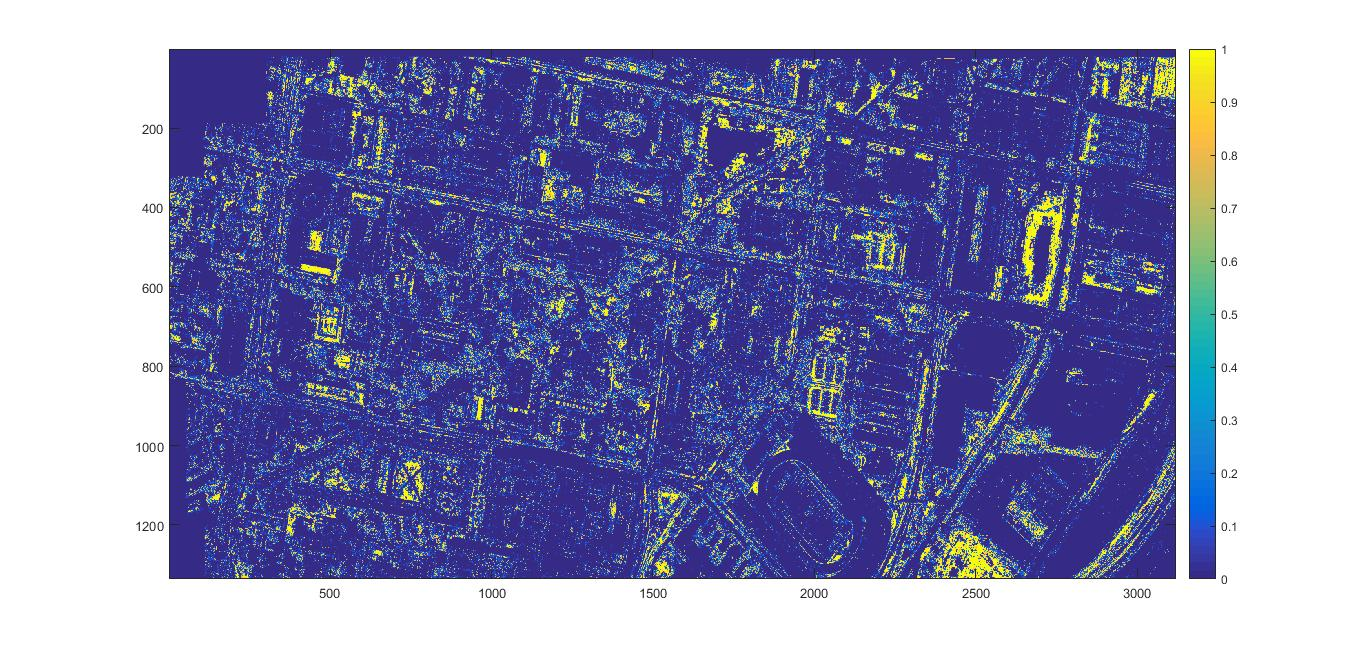
\includegraphics[trim={6cm 2.5cm 4.5cm 1.6cm},clip,scale=0.18]{1.jpg} & \vspace{-3cm}Gaussian Blur \\ 
\midrule 
\vspace{-3cm}
\hspace{-0.6cm}
K-means, K = 2 & 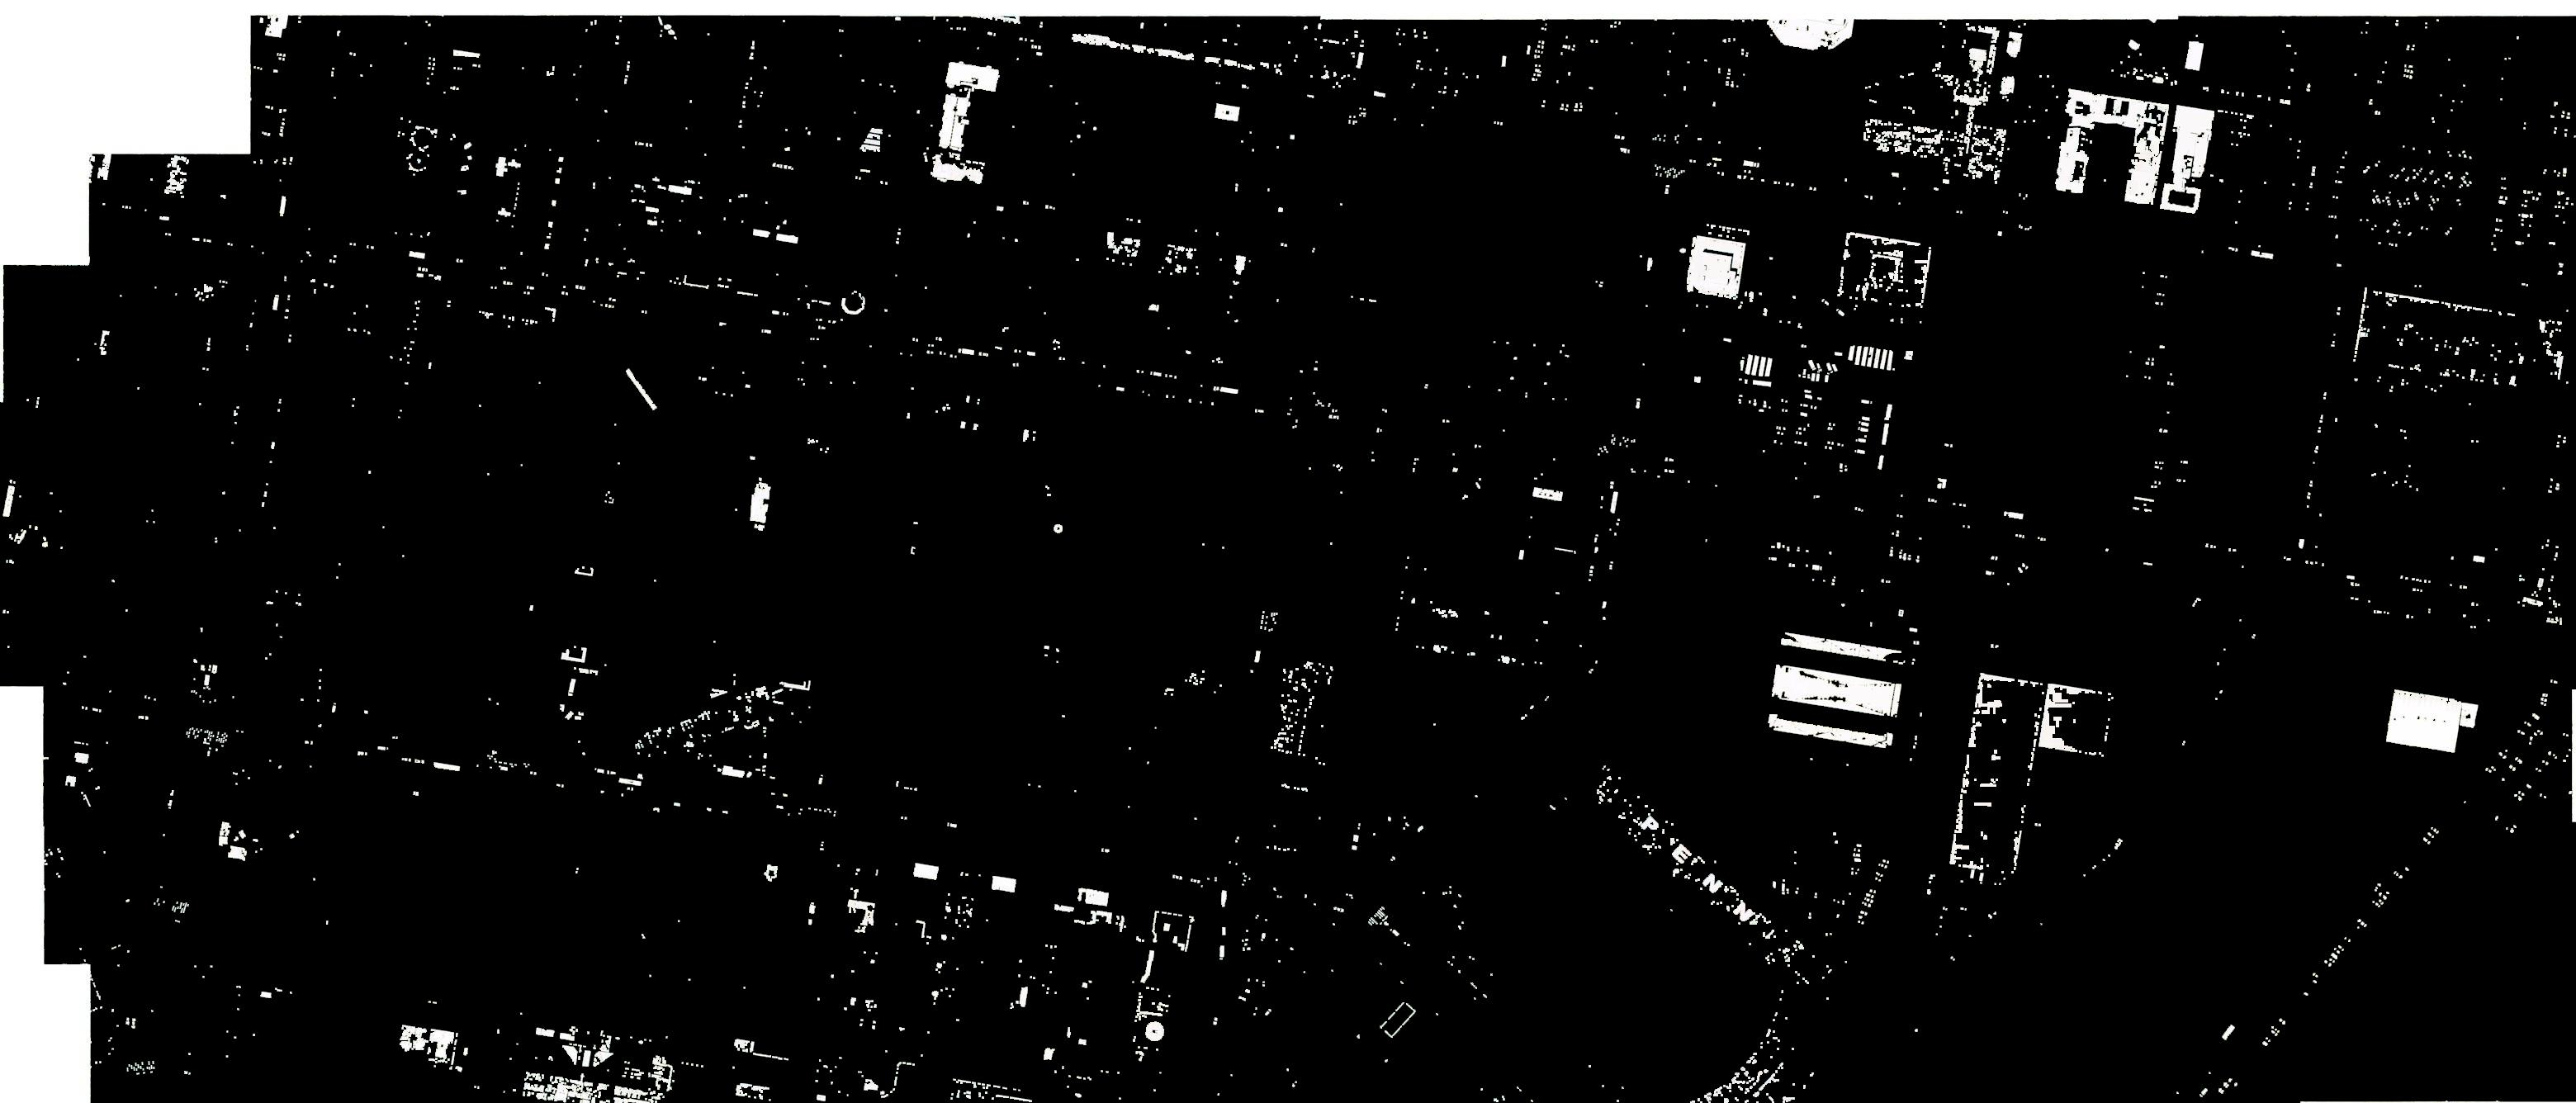
\includegraphics[clip,scale=0.07]{2rgb.jpg} & 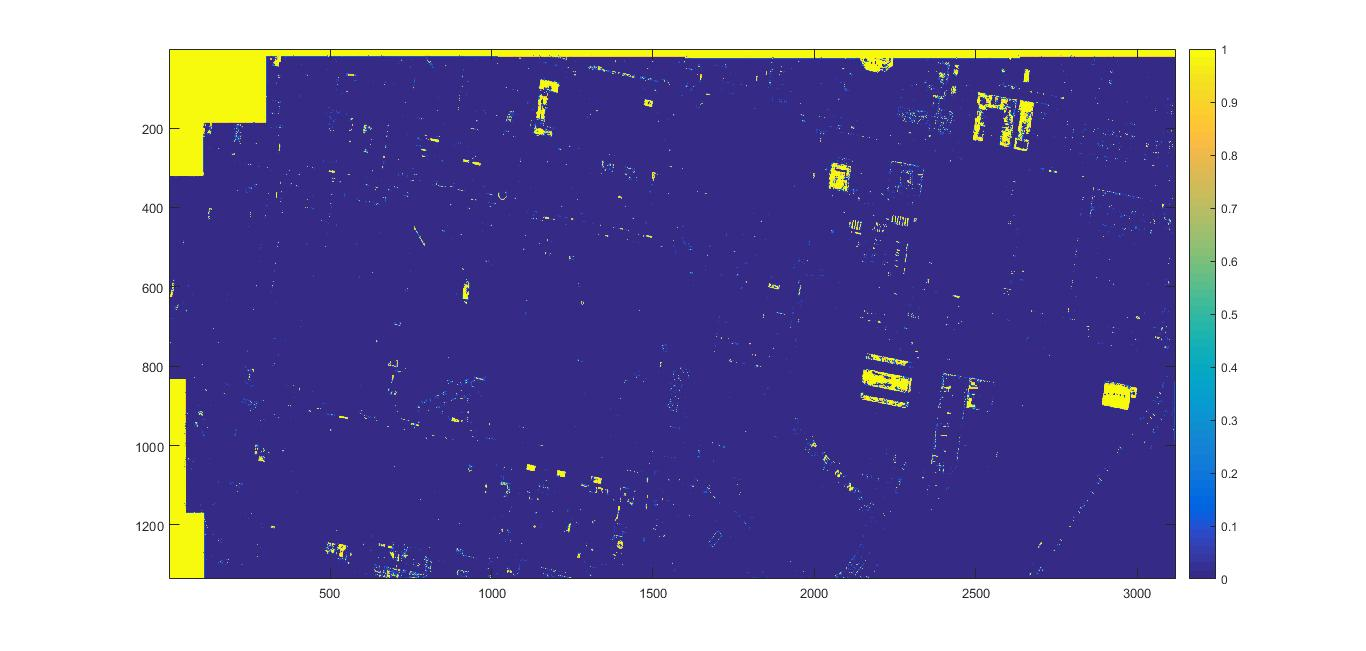
\includegraphics[trim={6cm 2.5cm 4.5cm 1.6cm},clip,scale=0.18]{2.jpg} & \vspace{-3cm}Gaussian Blur \\ 
\midrule 
\vspace{-3cm}
\hspace{-0.6cm}
K-means, K = 3 & 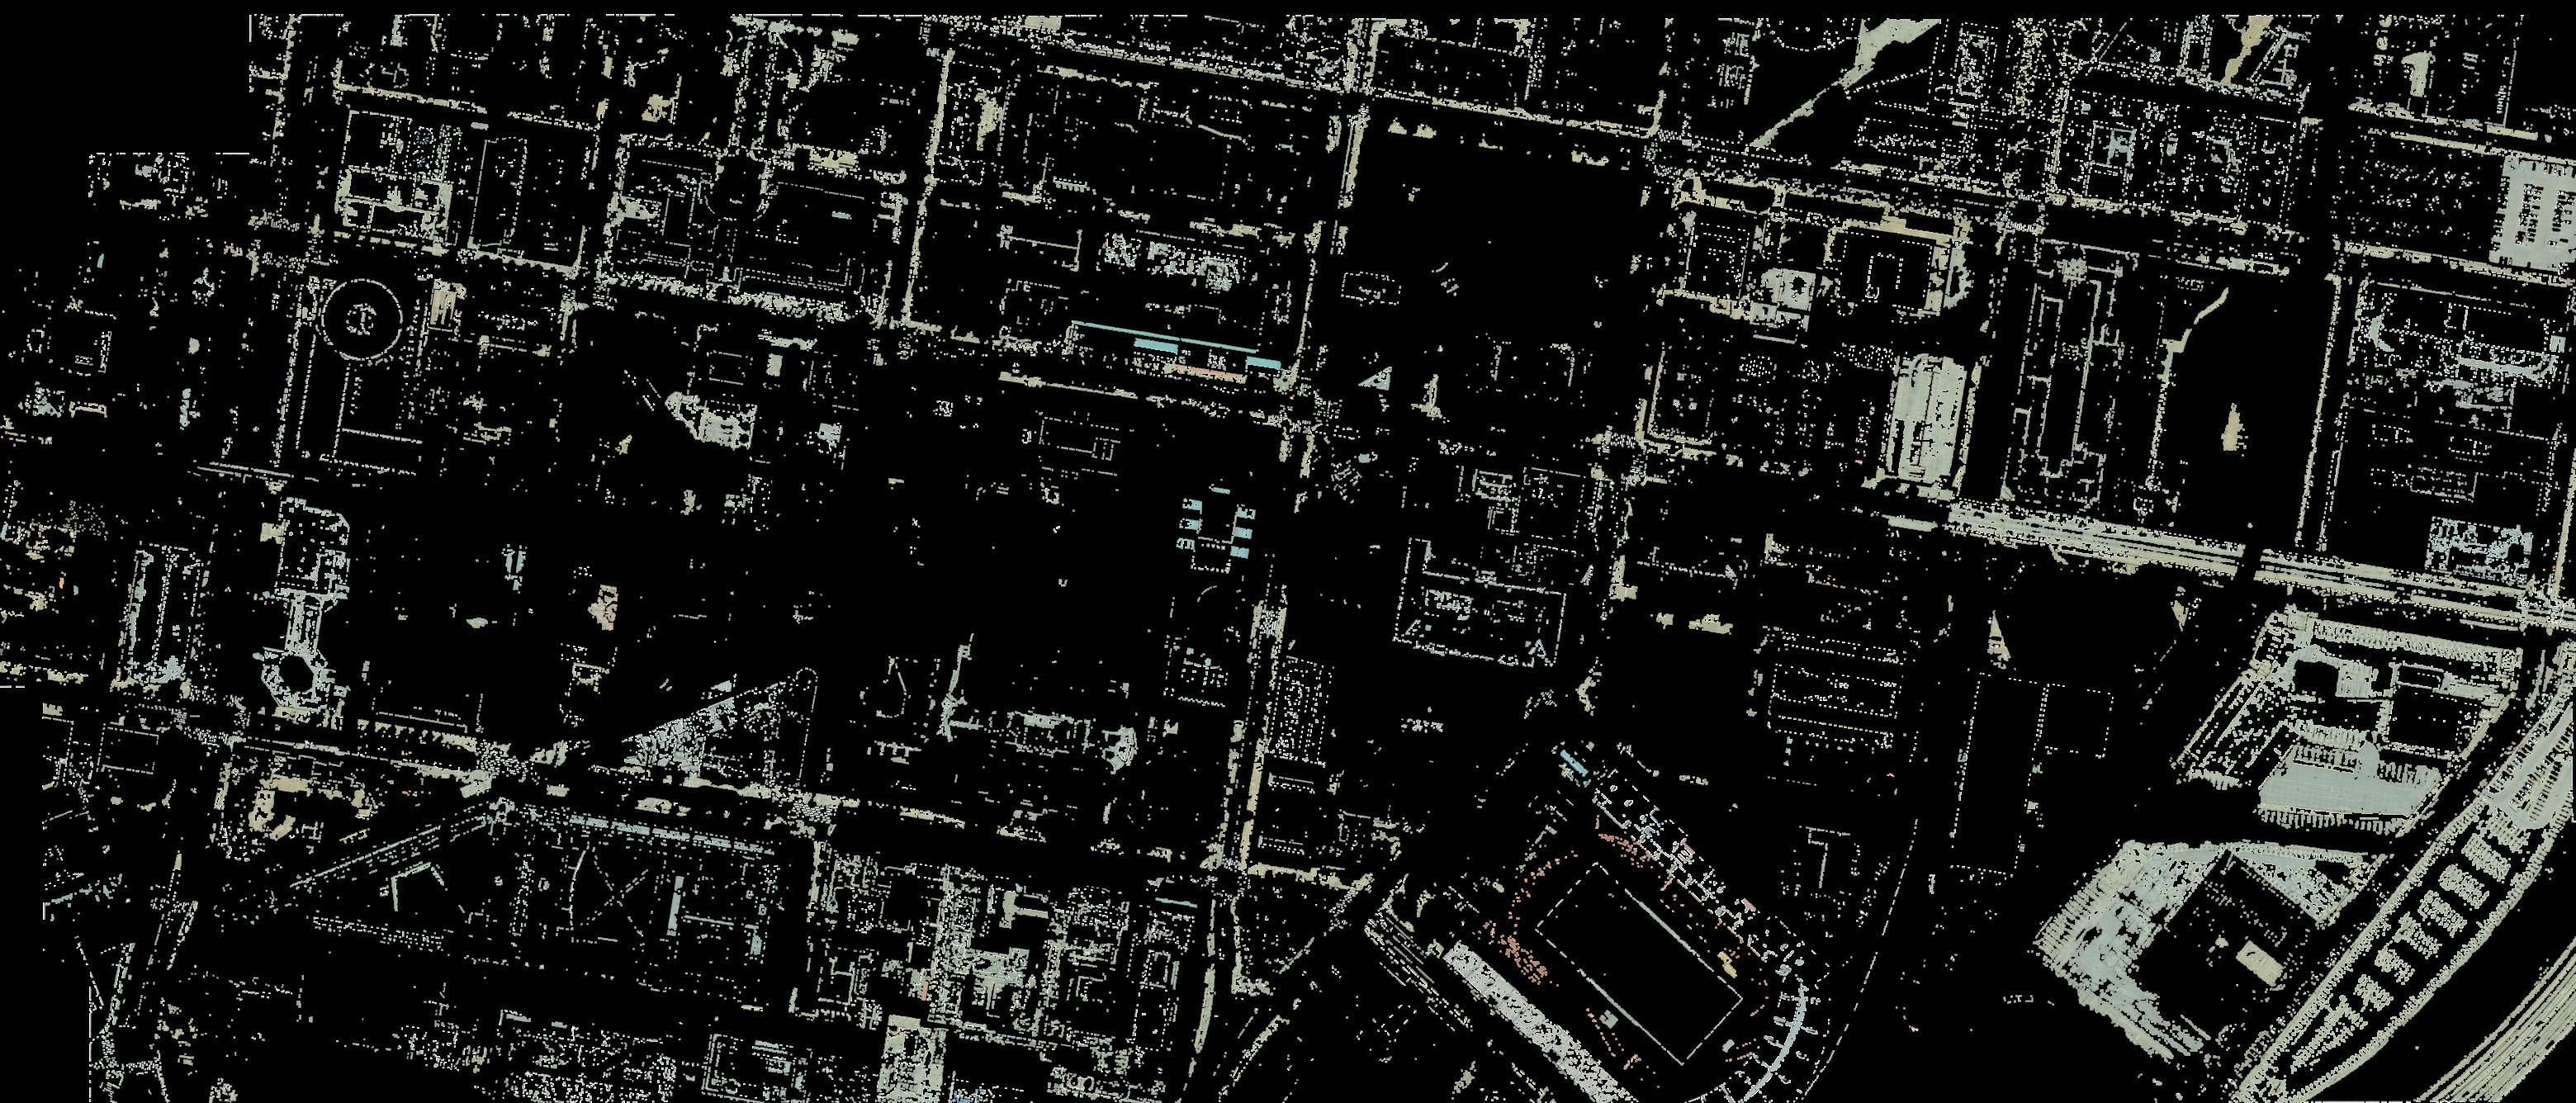
\includegraphics[clip,scale=0.07]{3rgb.jpg} & 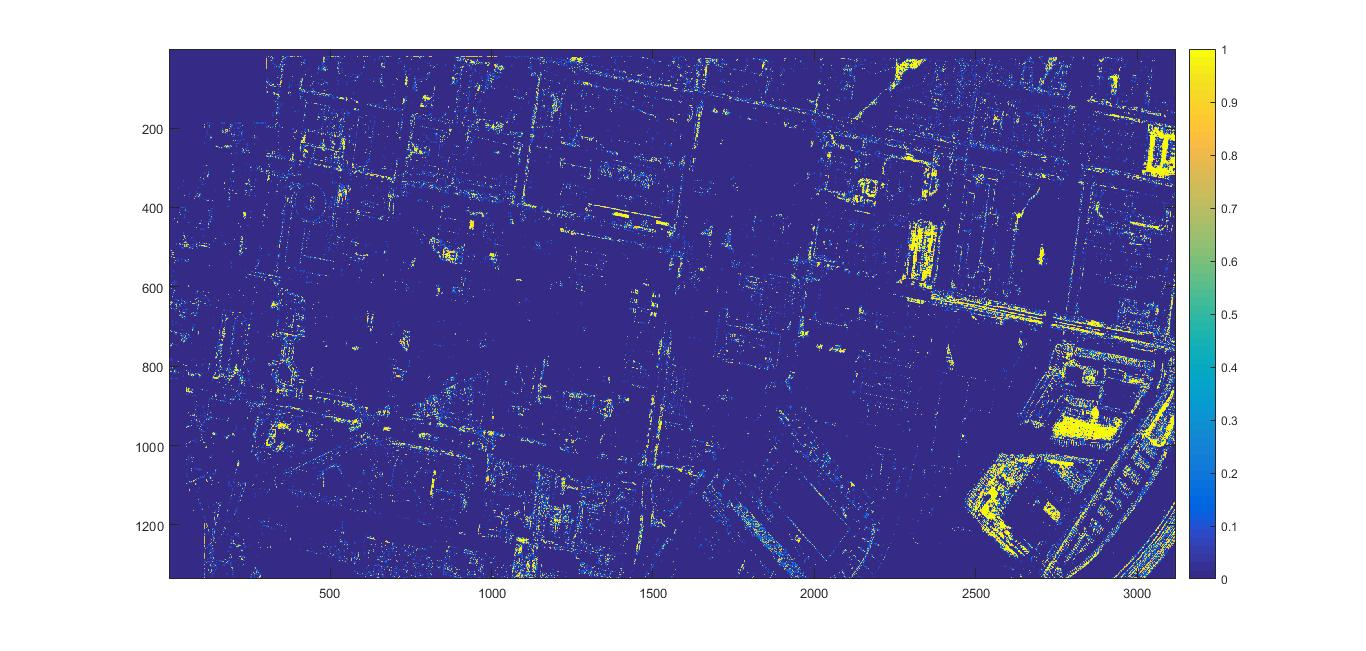
\includegraphics[trim={6cm 2.5cm 4.5cm 1.6cm},clip,scale=0.18]{3.jpg} & \vspace{-3cm}Gaussian Blur \\ 
\midrule 
\vspace{-3cm}
\hspace{-0.6cm}
K-means, K = 4 & 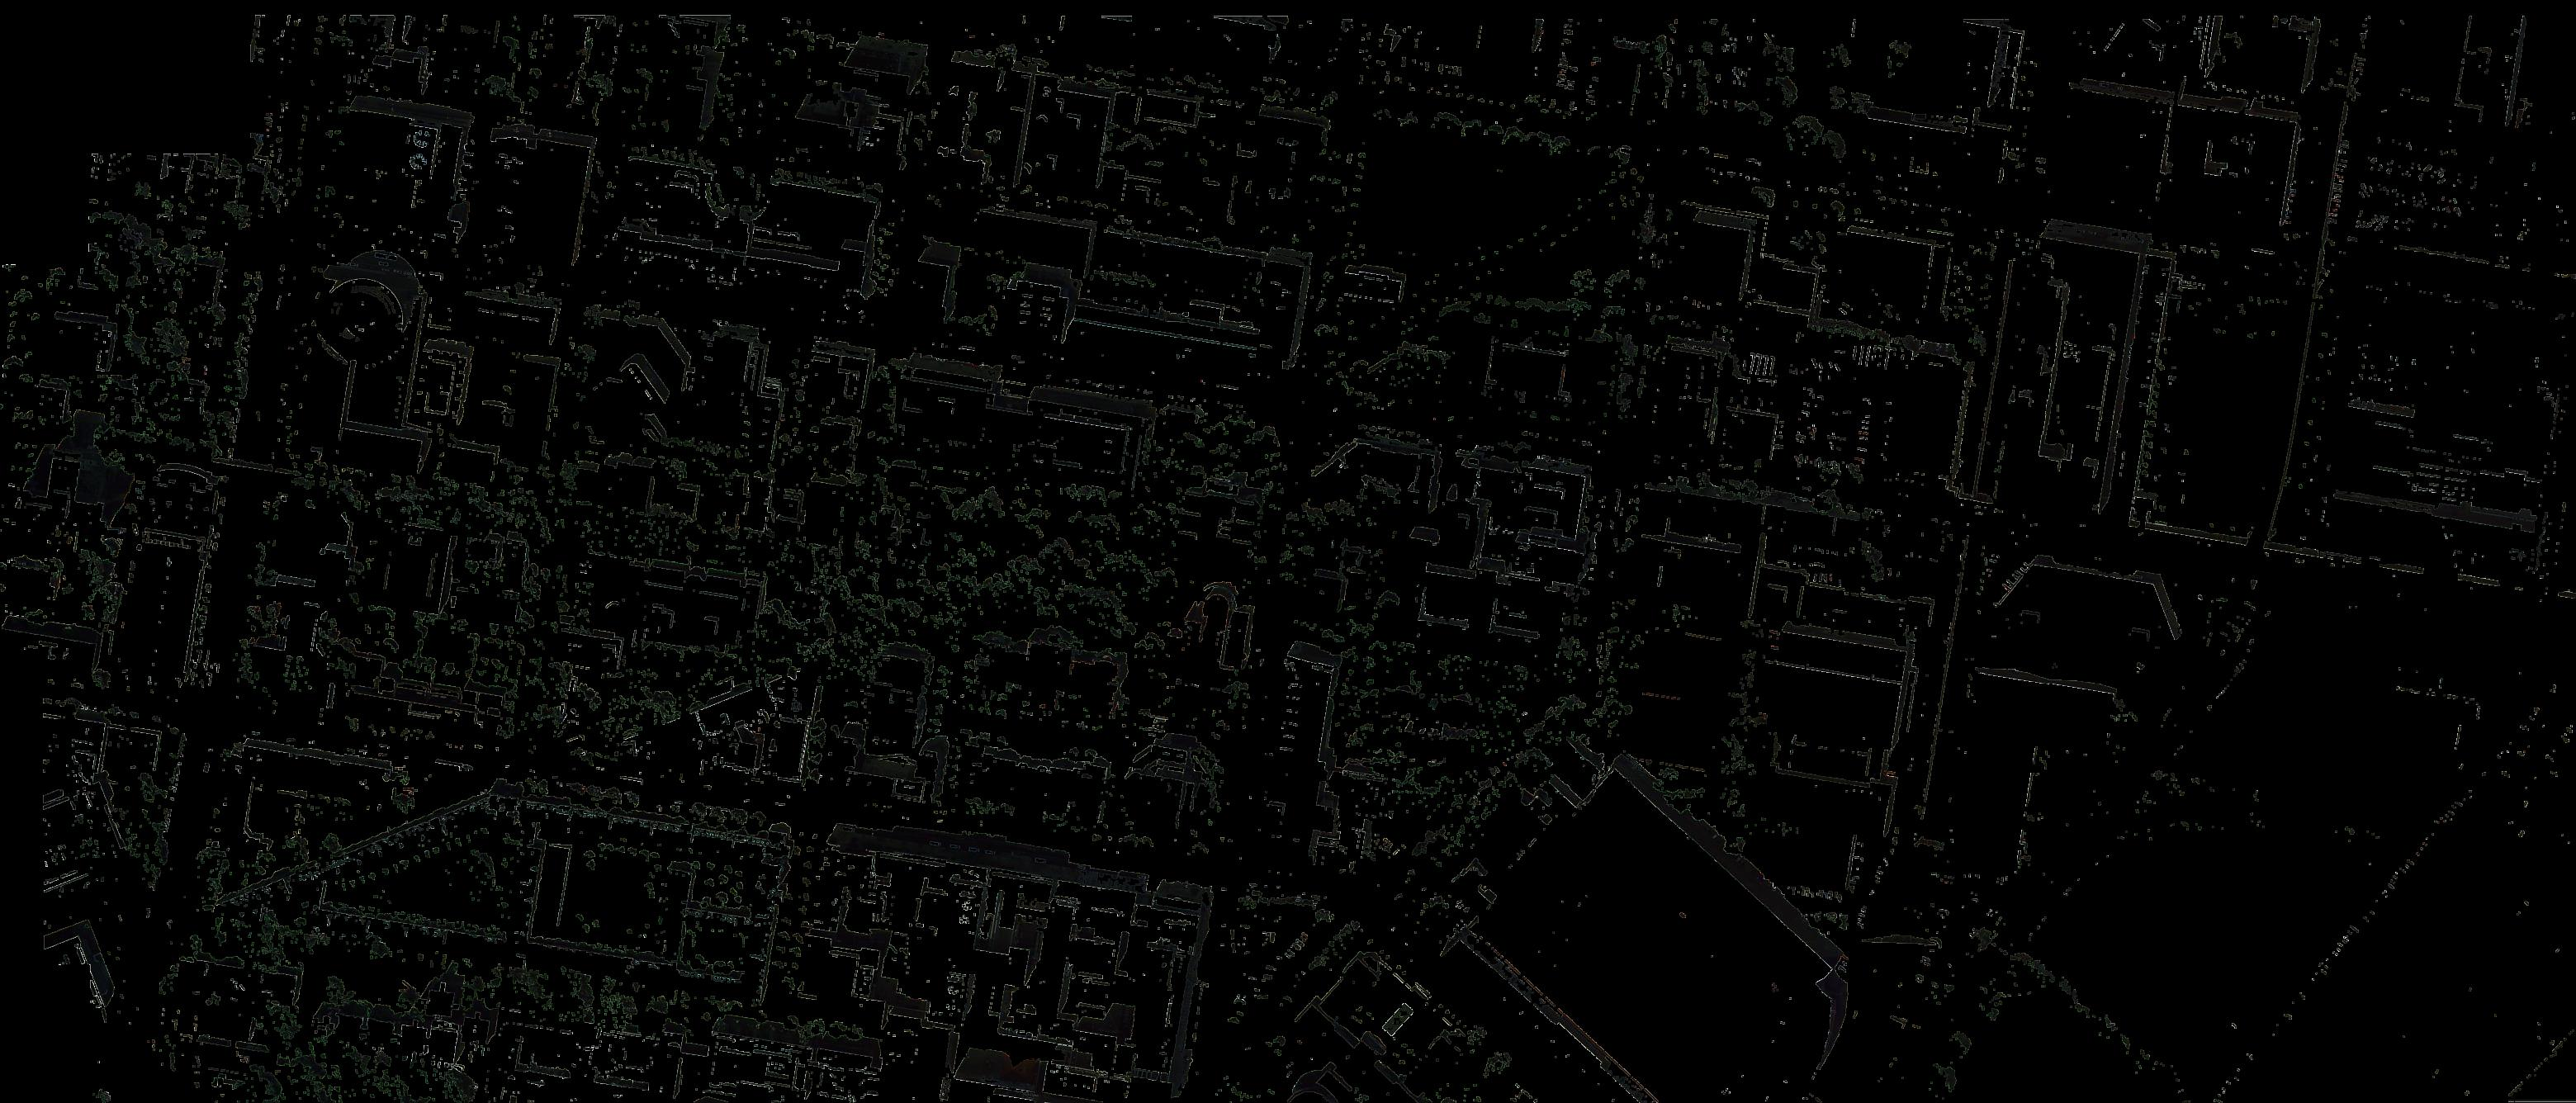
\includegraphics[clip,scale=0.07]{4rgb.jpg} & 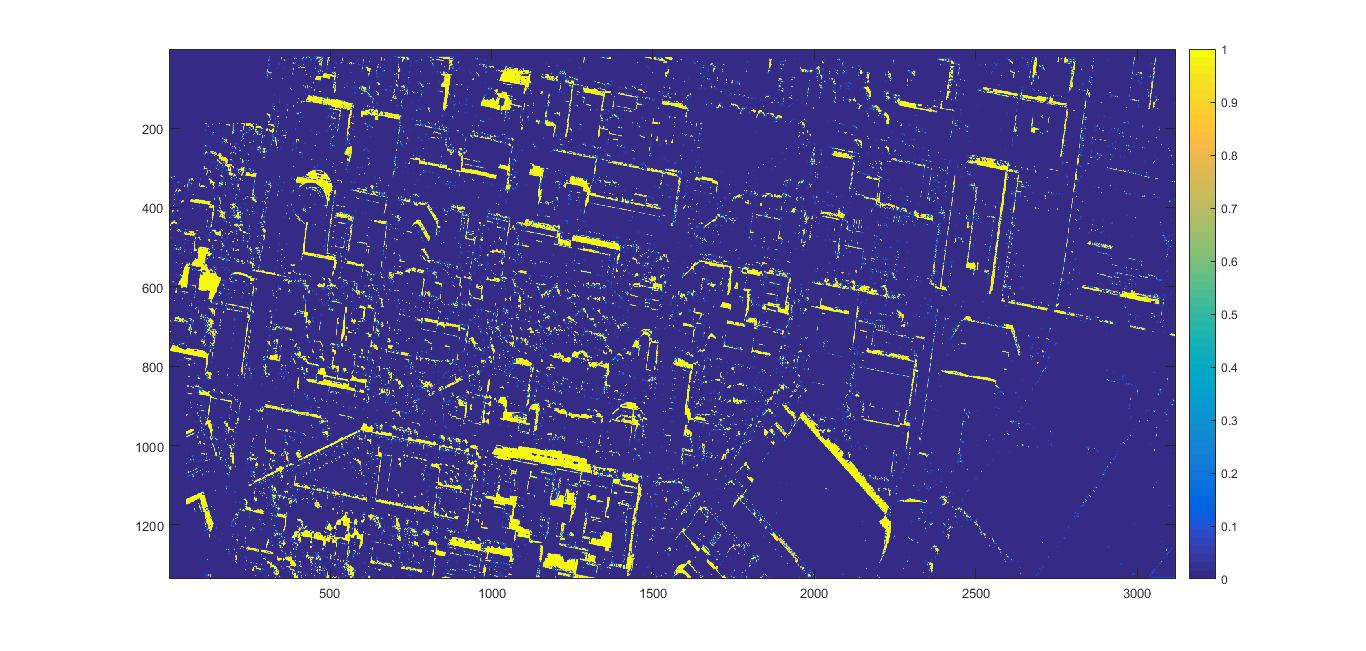
\includegraphics[trim={6cm 2.5cm 4.5cm 1.6cm},clip,scale=0.18]{4.jpg} & \vspace{-3cm}Gaussian Blur \\ 
\midrule 
\vspace{-3cm}
\hspace{-0.6cm}
K-means, K = 5 & 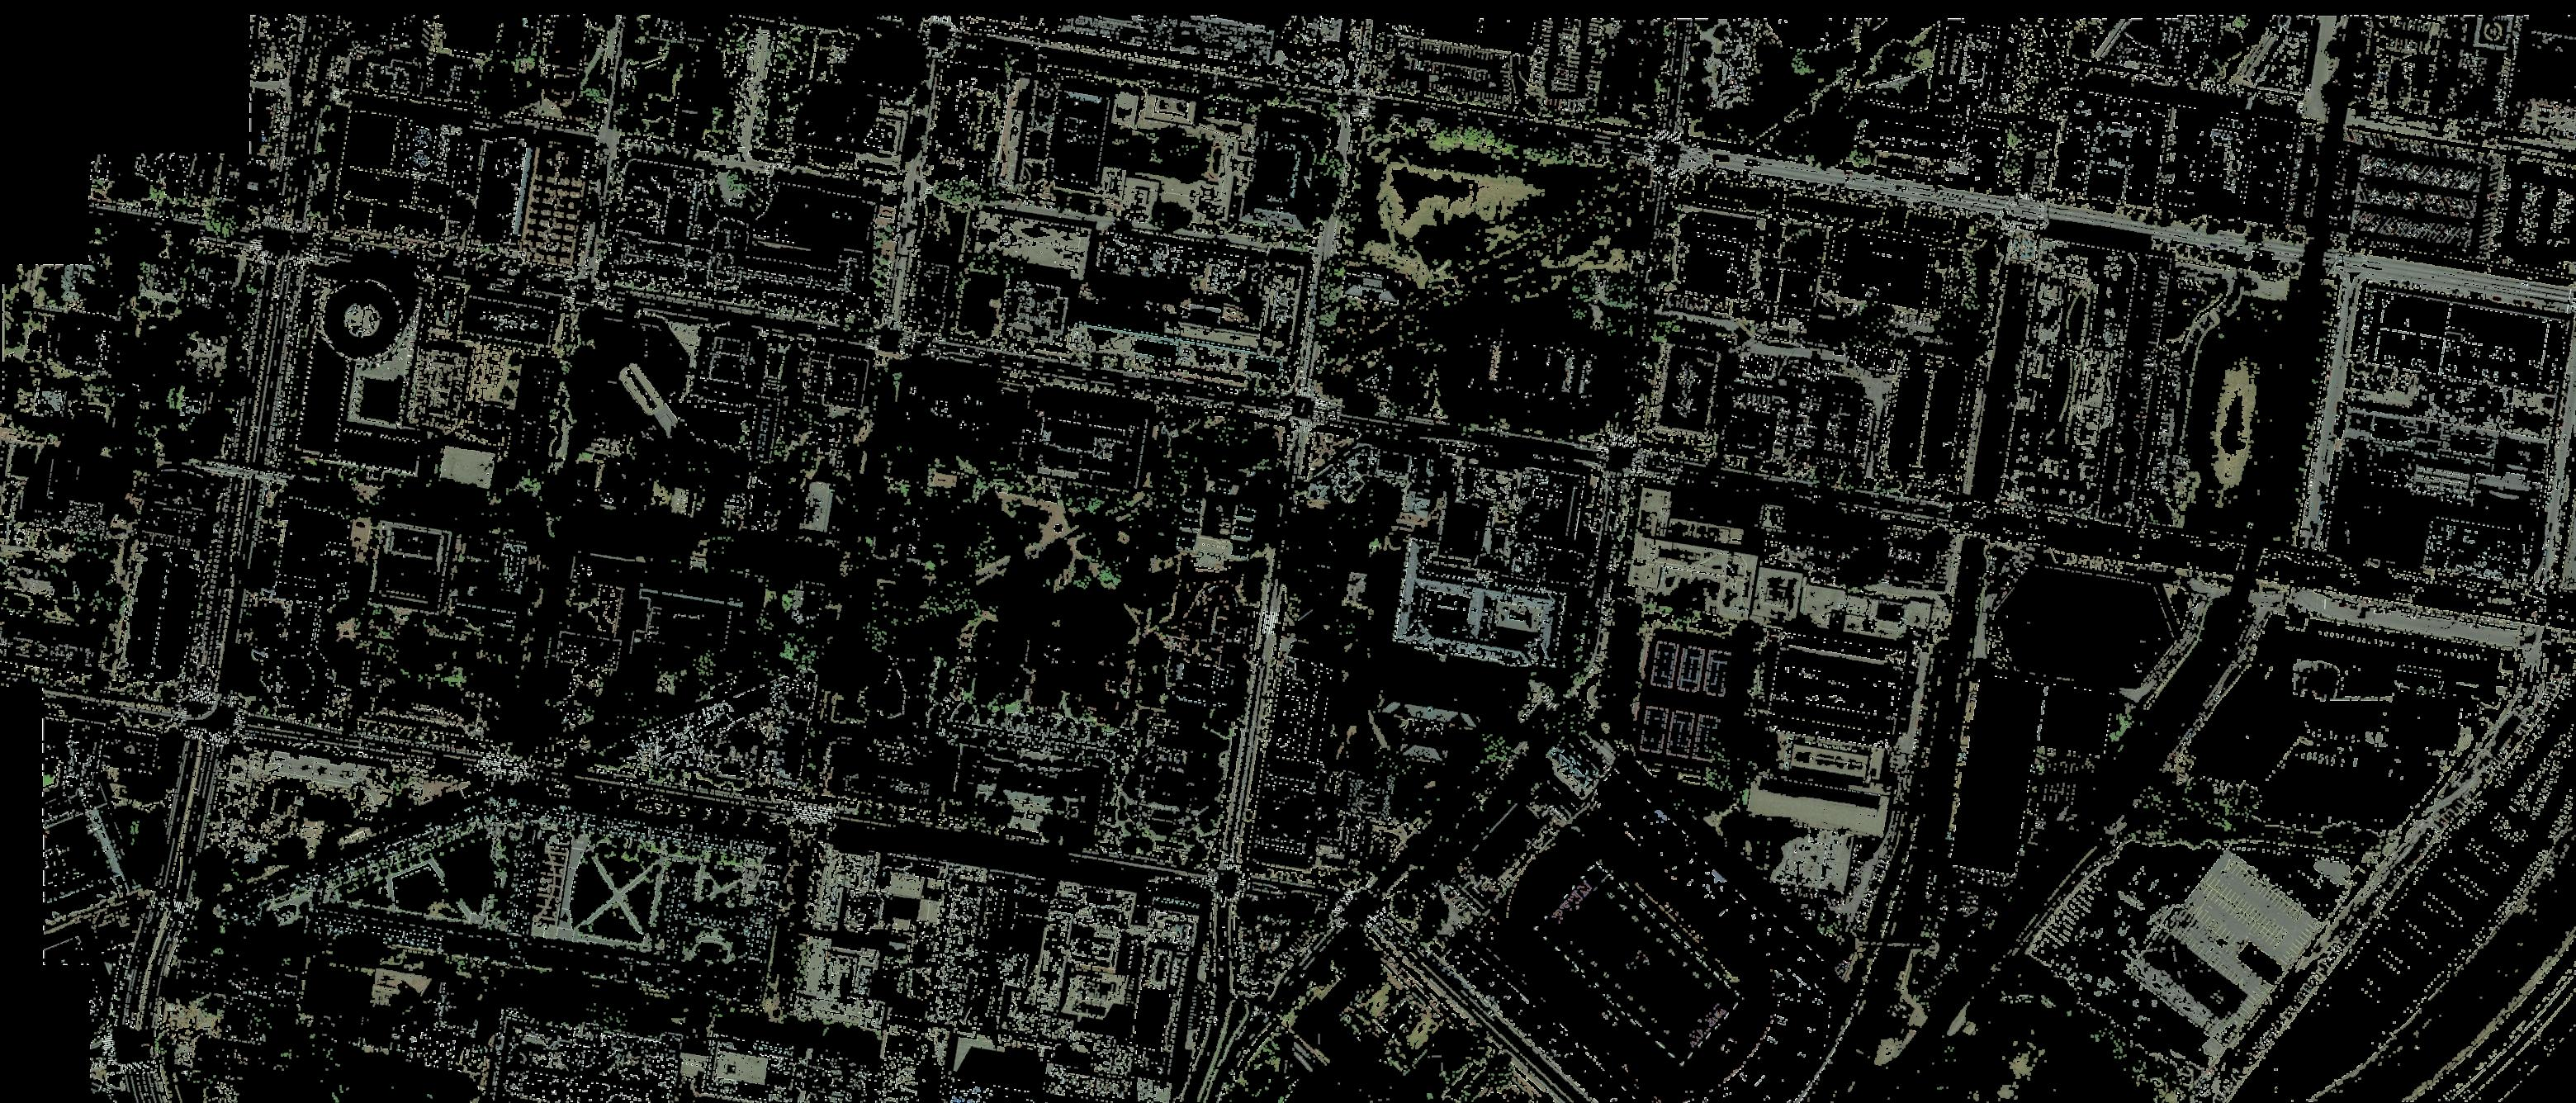
\includegraphics[clip,scale=0.07]{5rgb.jpg} & 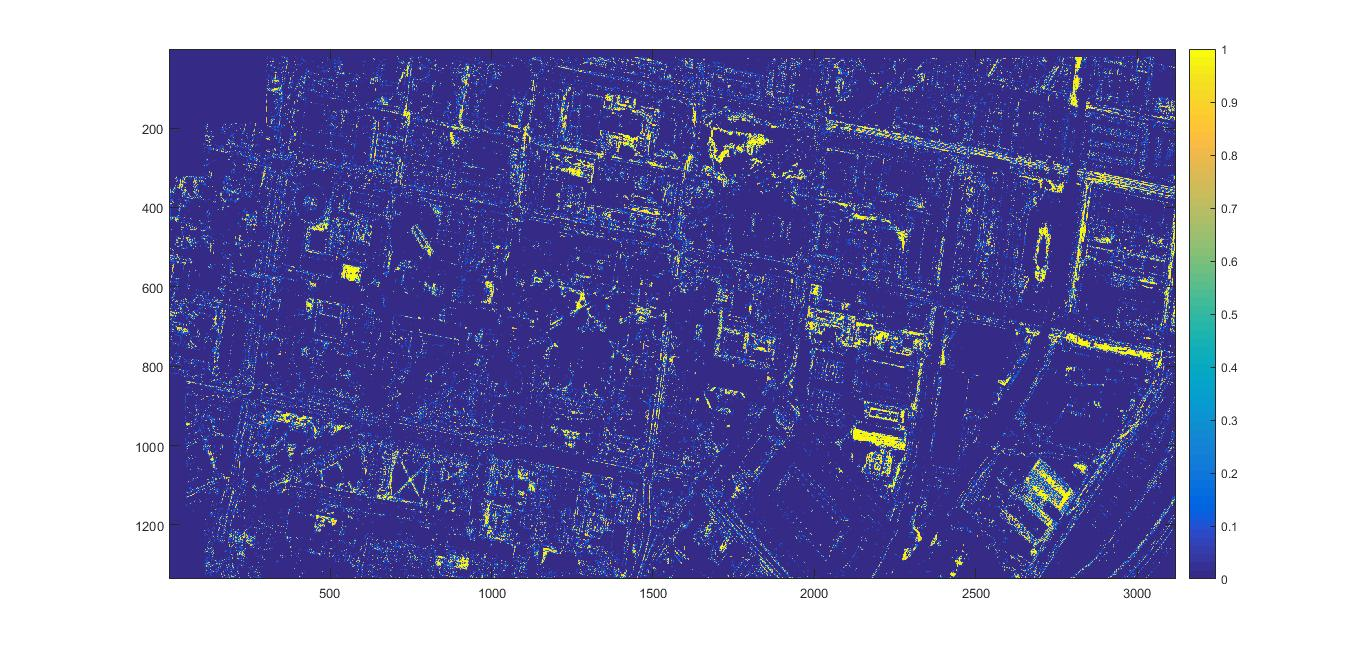
\includegraphics[trim={6cm 2.5cm 4.5cm 1.6cm},clip,scale=0.18]{5.jpg} & \vspace{-3cm}Gaussian Blur \\ 
\midrule 
\vspace{-3cm}
\hspace{-0.6cm}
K-means, K = 6 & 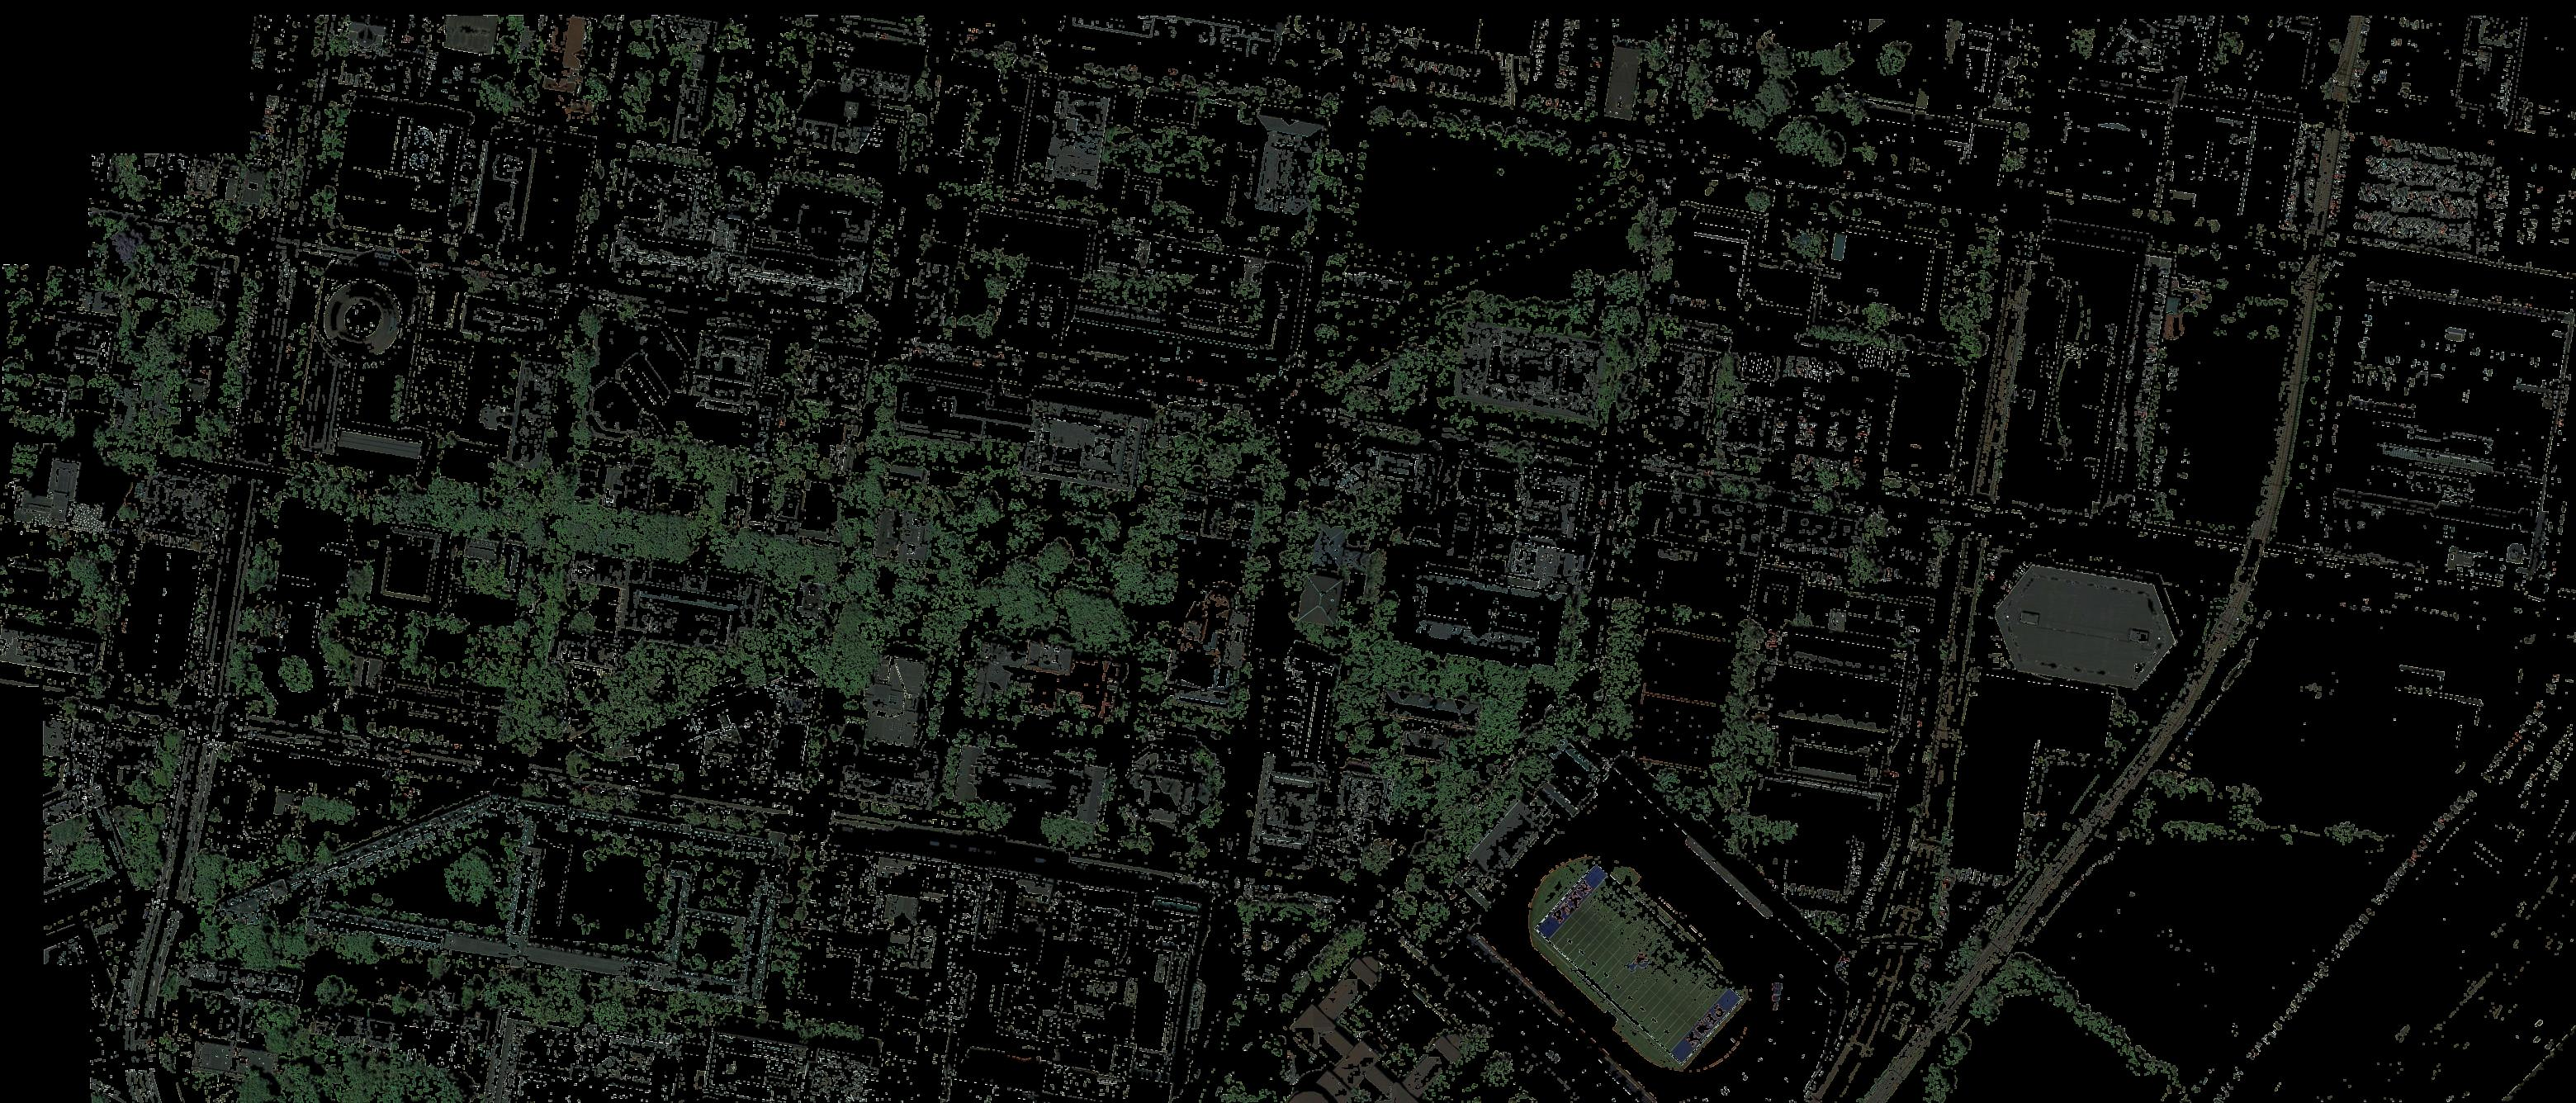
\includegraphics[clip,scale=0.07]{6rgb.jpg} & 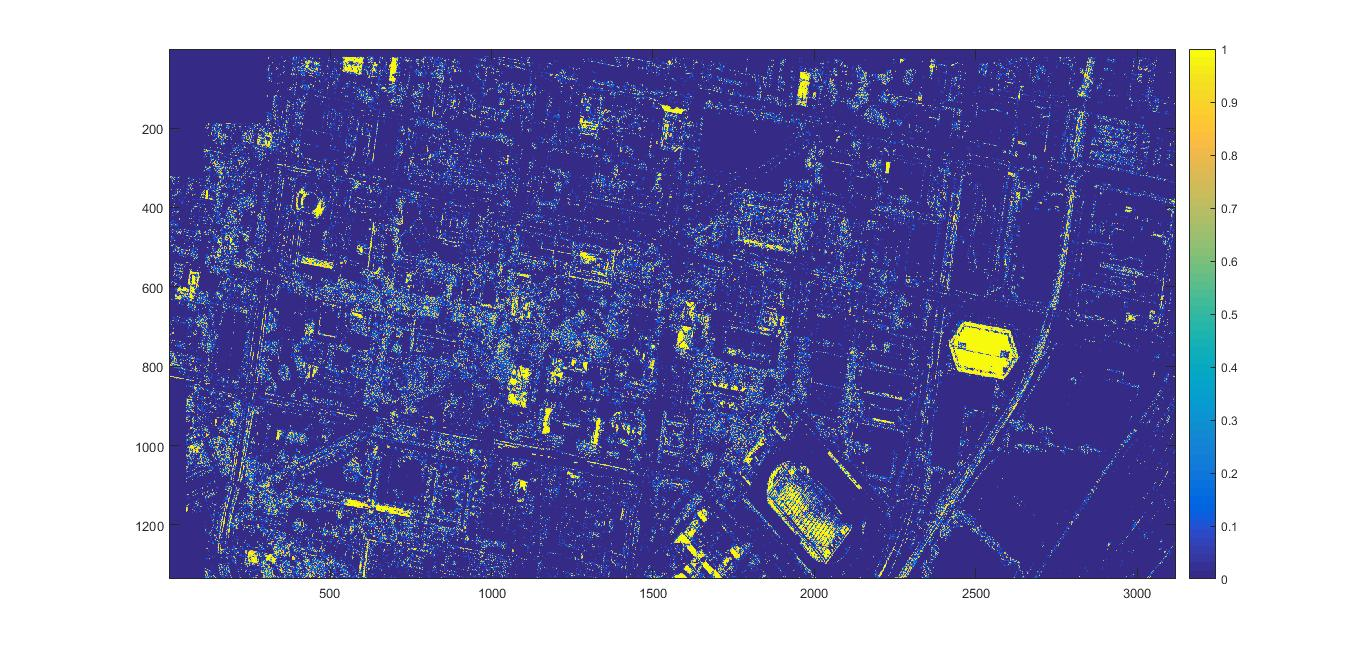
\includegraphics[trim={6cm 2.5cm 4.5cm 1.6cm},clip,scale=0.18]{6.jpg} & \vspace{-3cm}Gaussian Blur \\ 
\bottomrule
\end{tabular} 
\end{table*}

\begin{table*}
\centering
\begin{tabular}{>{\centering\arraybackslash}M{8mm}cc>{\centering\arraybackslash}M{20mm}}
\toprule
Feature & Masked RGB Image & Feature & Post Processing \\ 
\midrule 
\vspace{-3cm}
\hspace{-0.6cm}
K-means, K = 7 & 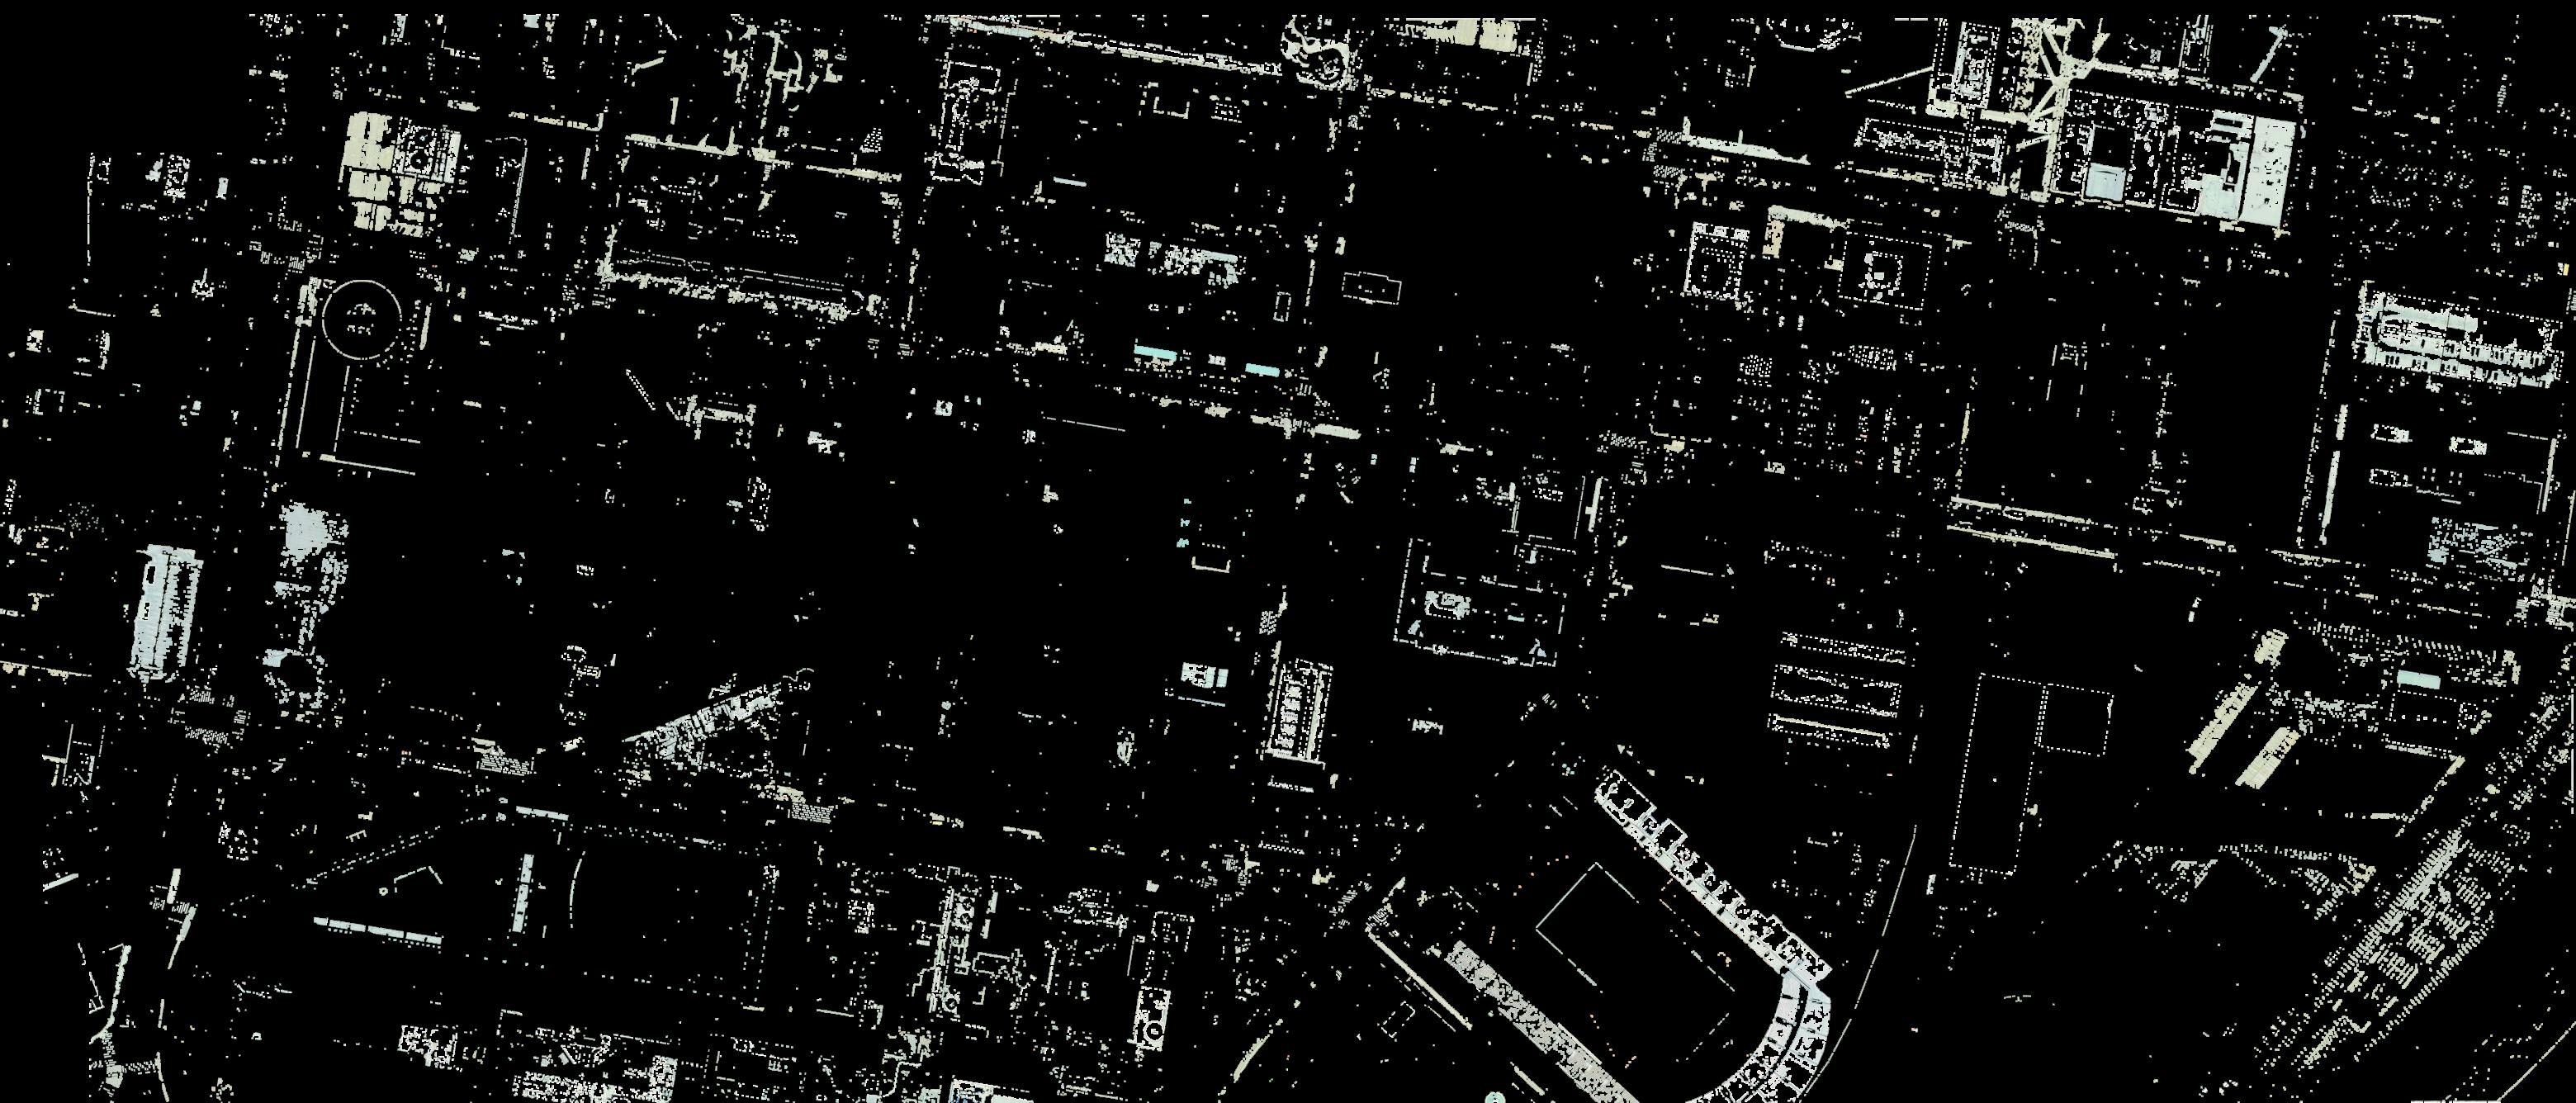
\includegraphics[clip,scale=0.07]{7rgb.jpg} & 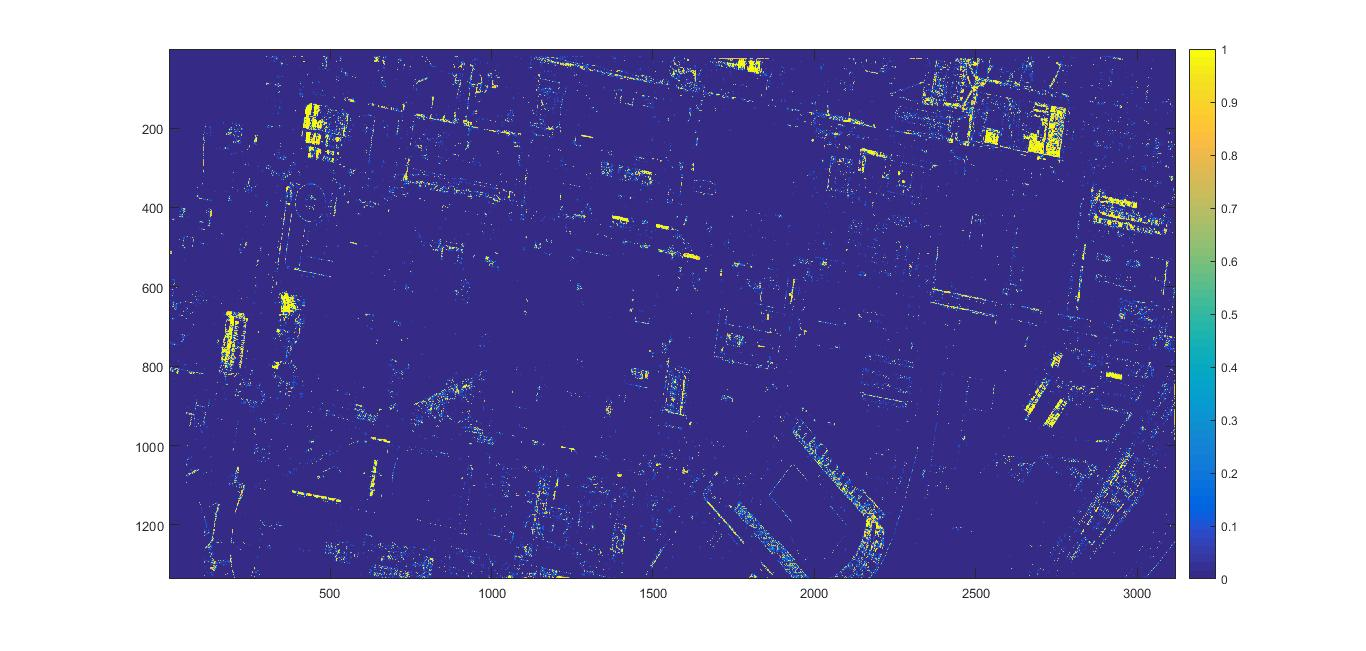
\includegraphics[trim={6cm 2.5cm 4.5cm 1.6cm},clip,scale=0.18]{7.jpg} & \vspace{-3cm}Gaussian Blur \\ 
\midrule 
\vspace{-3cm}
\hspace{-0.6cm}
K-means, K = 8 & 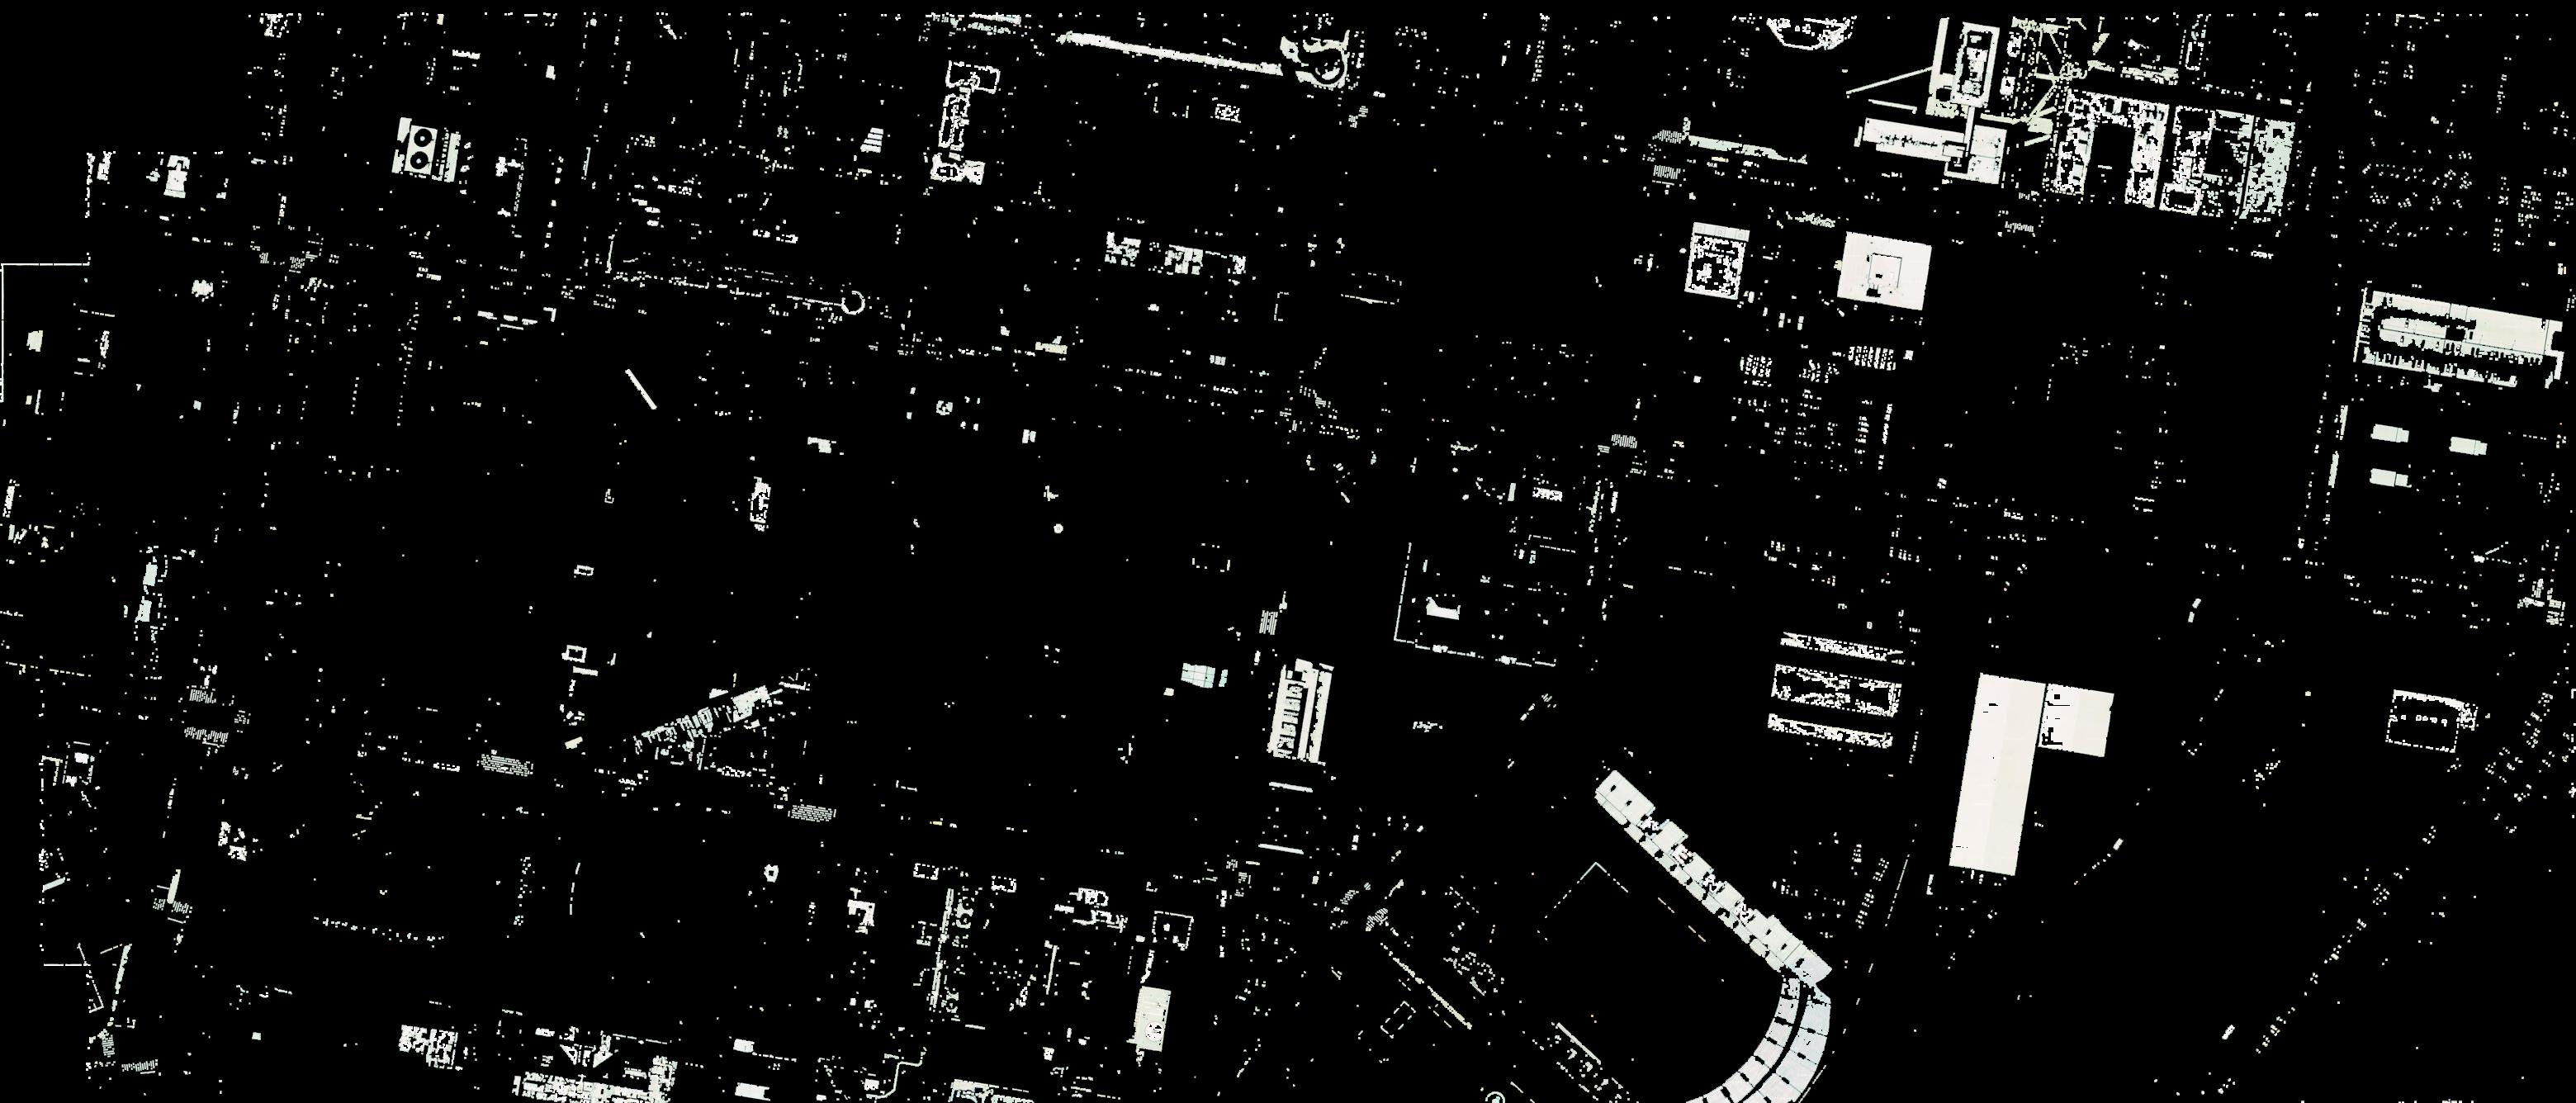
\includegraphics[clip,scale=0.07]{8rgb.jpg} & 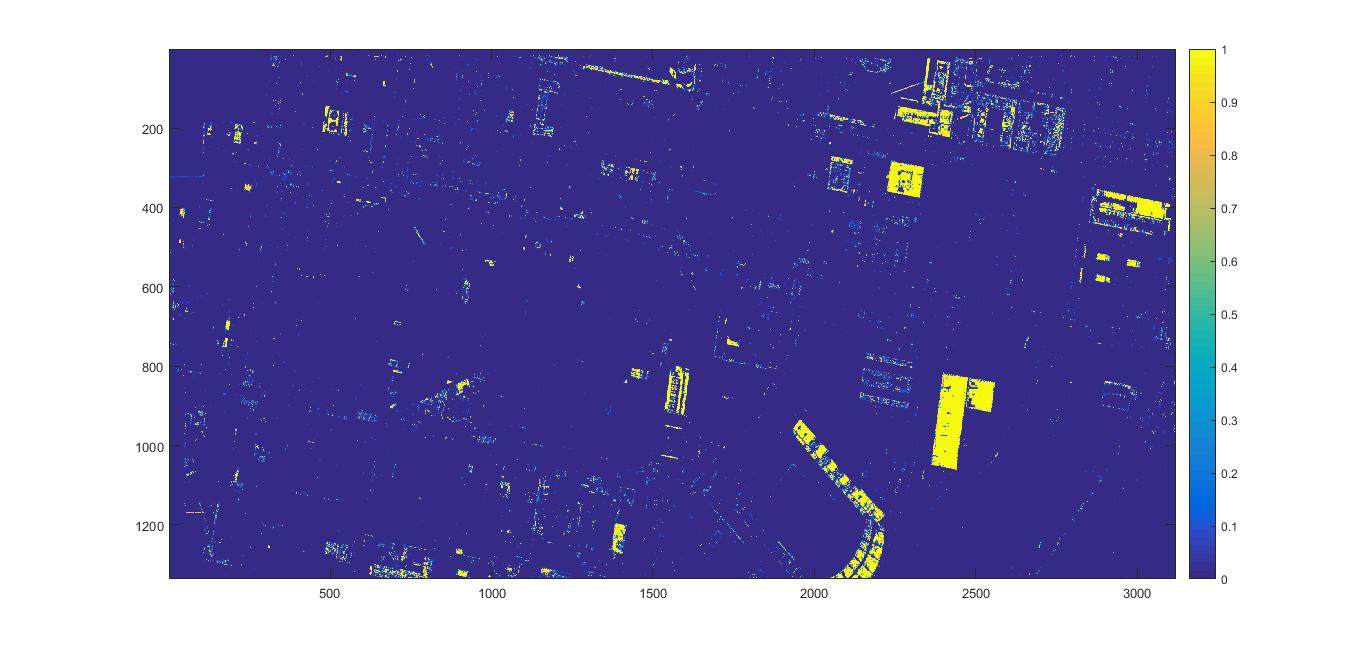
\includegraphics[trim={6cm 2.5cm 4.5cm 1.6cm},clip,scale=0.18]{8.jpg} & \vspace{-3cm}Gaussian Blur \\ 
\midrule 
\vspace{-3cm}
\hspace{-0.6cm}
K-means, K = 9 & 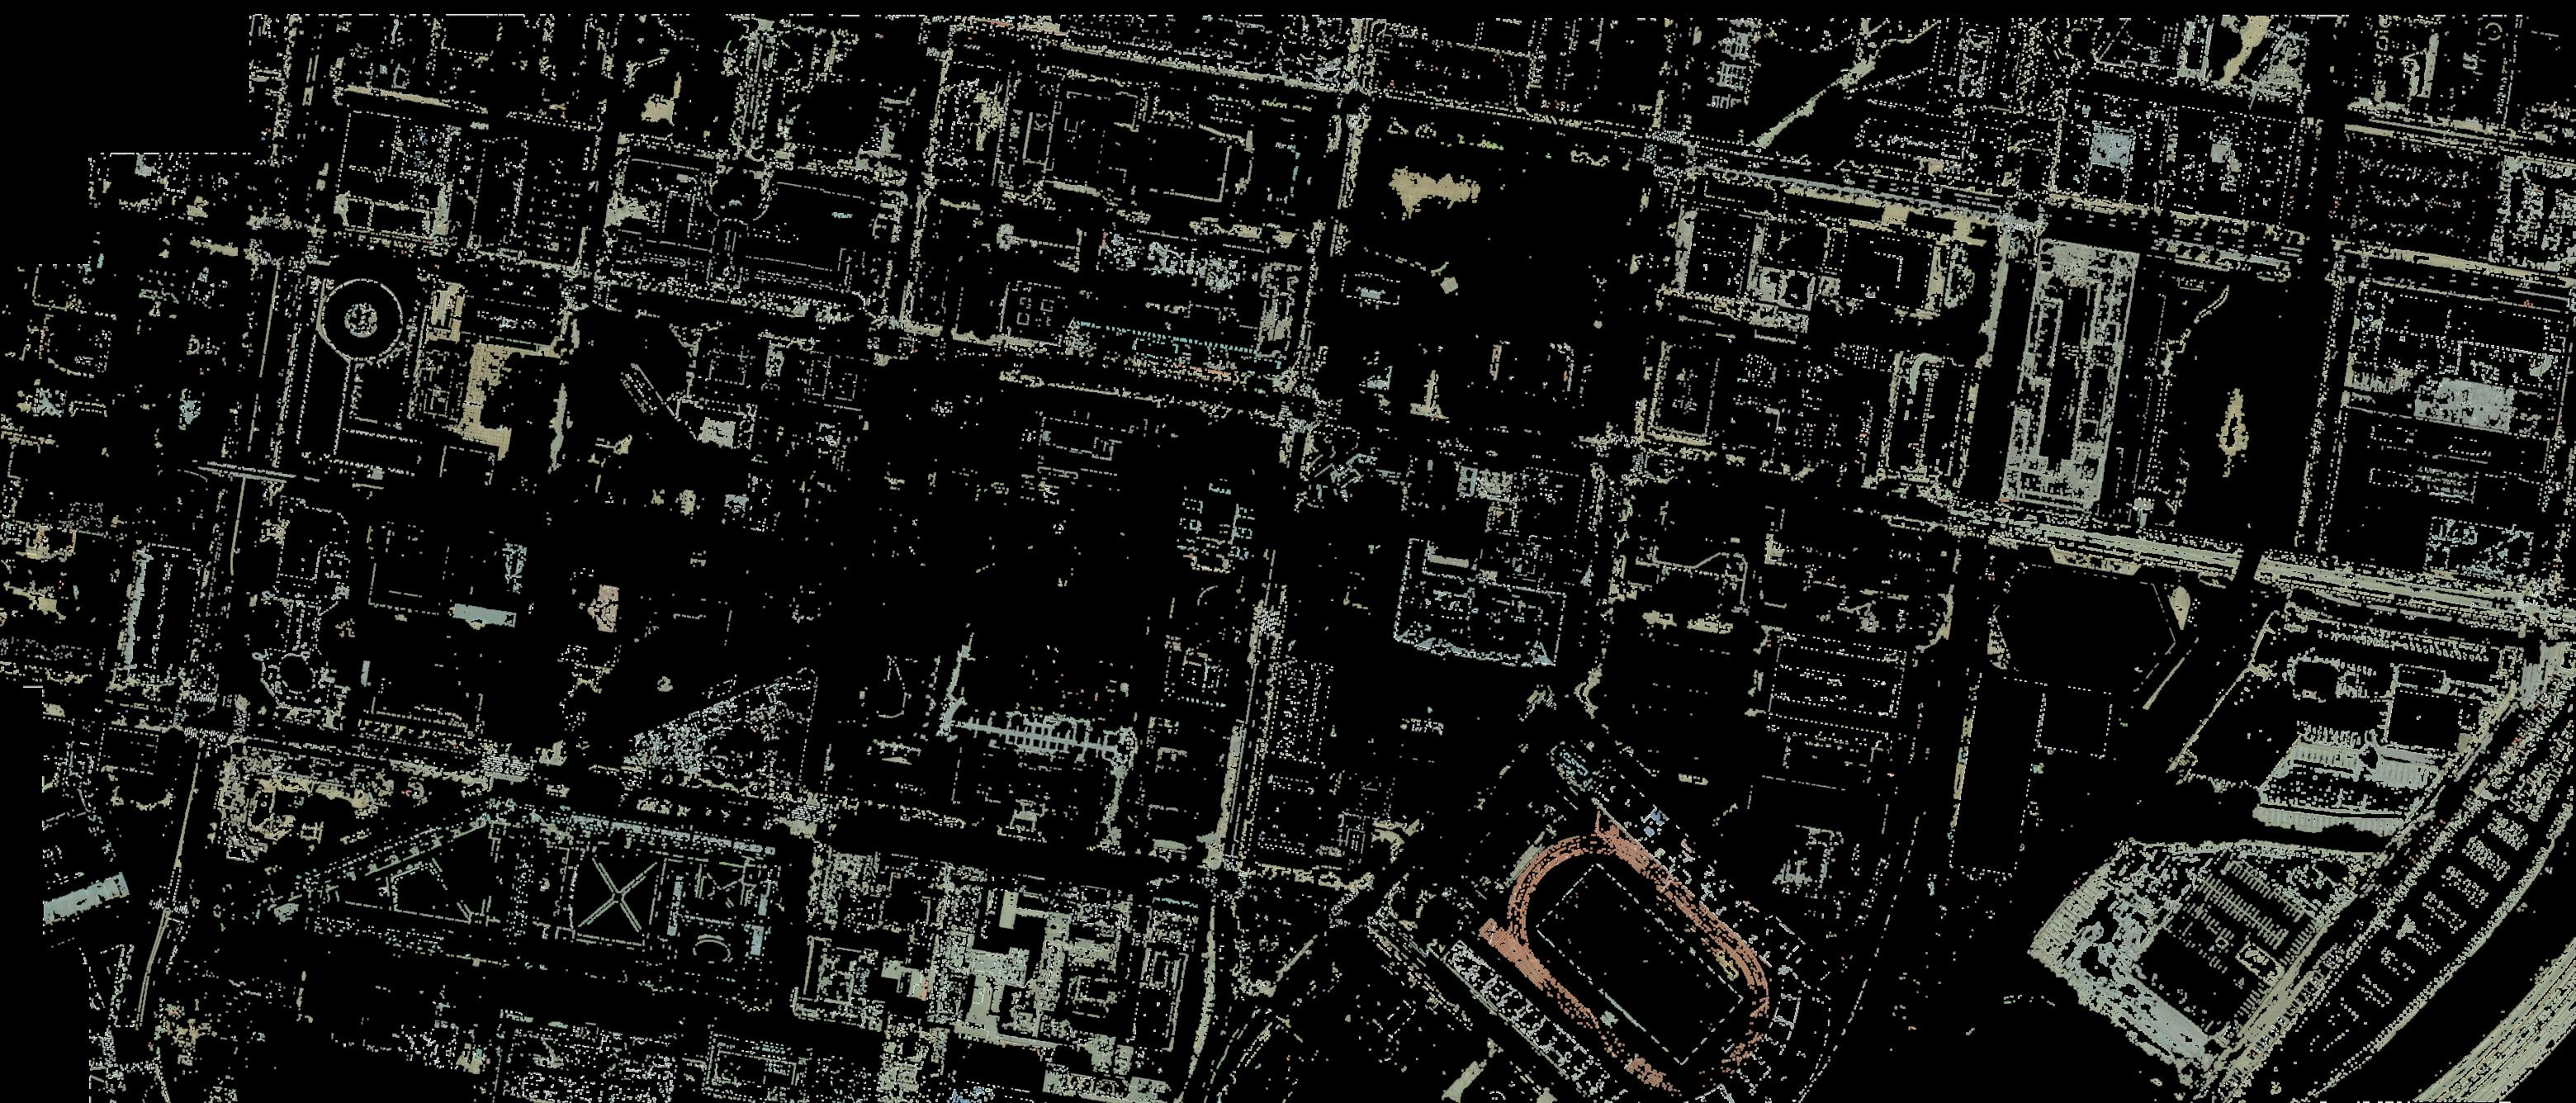
\includegraphics[clip,scale=0.07]{9rgb.jpg} & 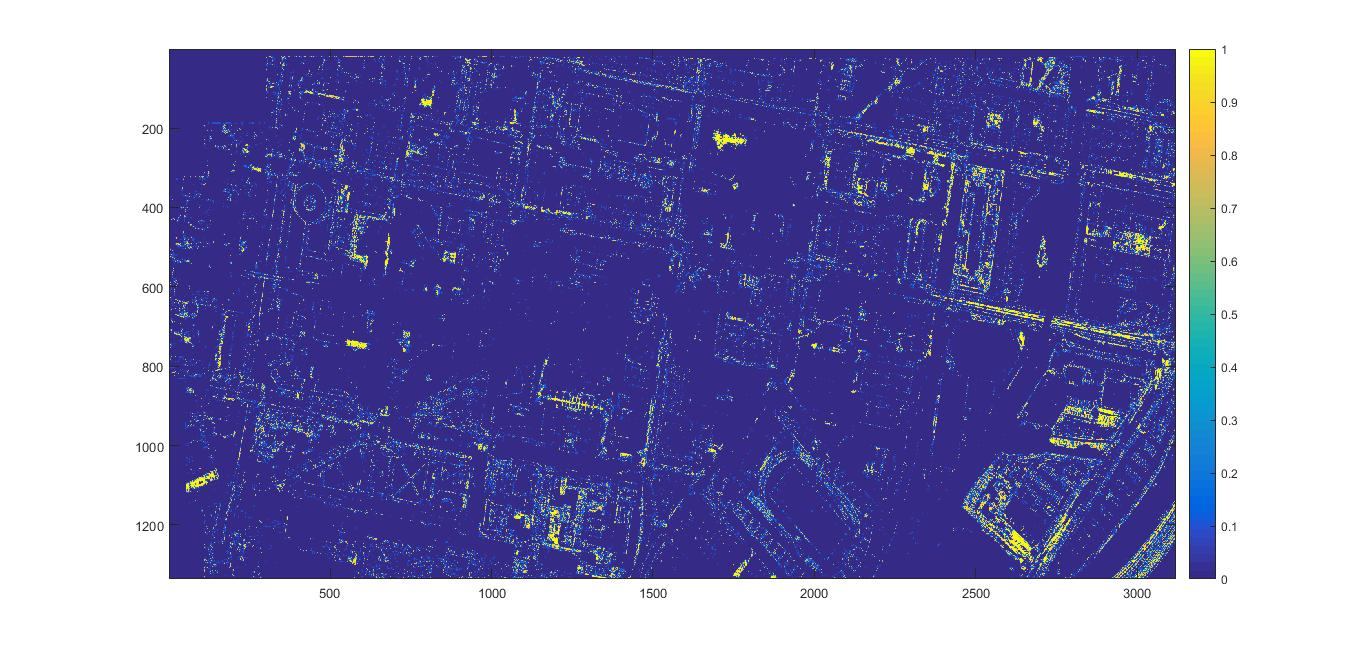
\includegraphics[trim={6cm 2.5cm 4.5cm 1.6cm},clip,scale=0.18]{9.jpg} & \vspace{-3cm}Gaussian Blur \\ 
\midrule 
\vspace{-3cm}
\hspace{-0.6cm}
K-means, K = 10 & 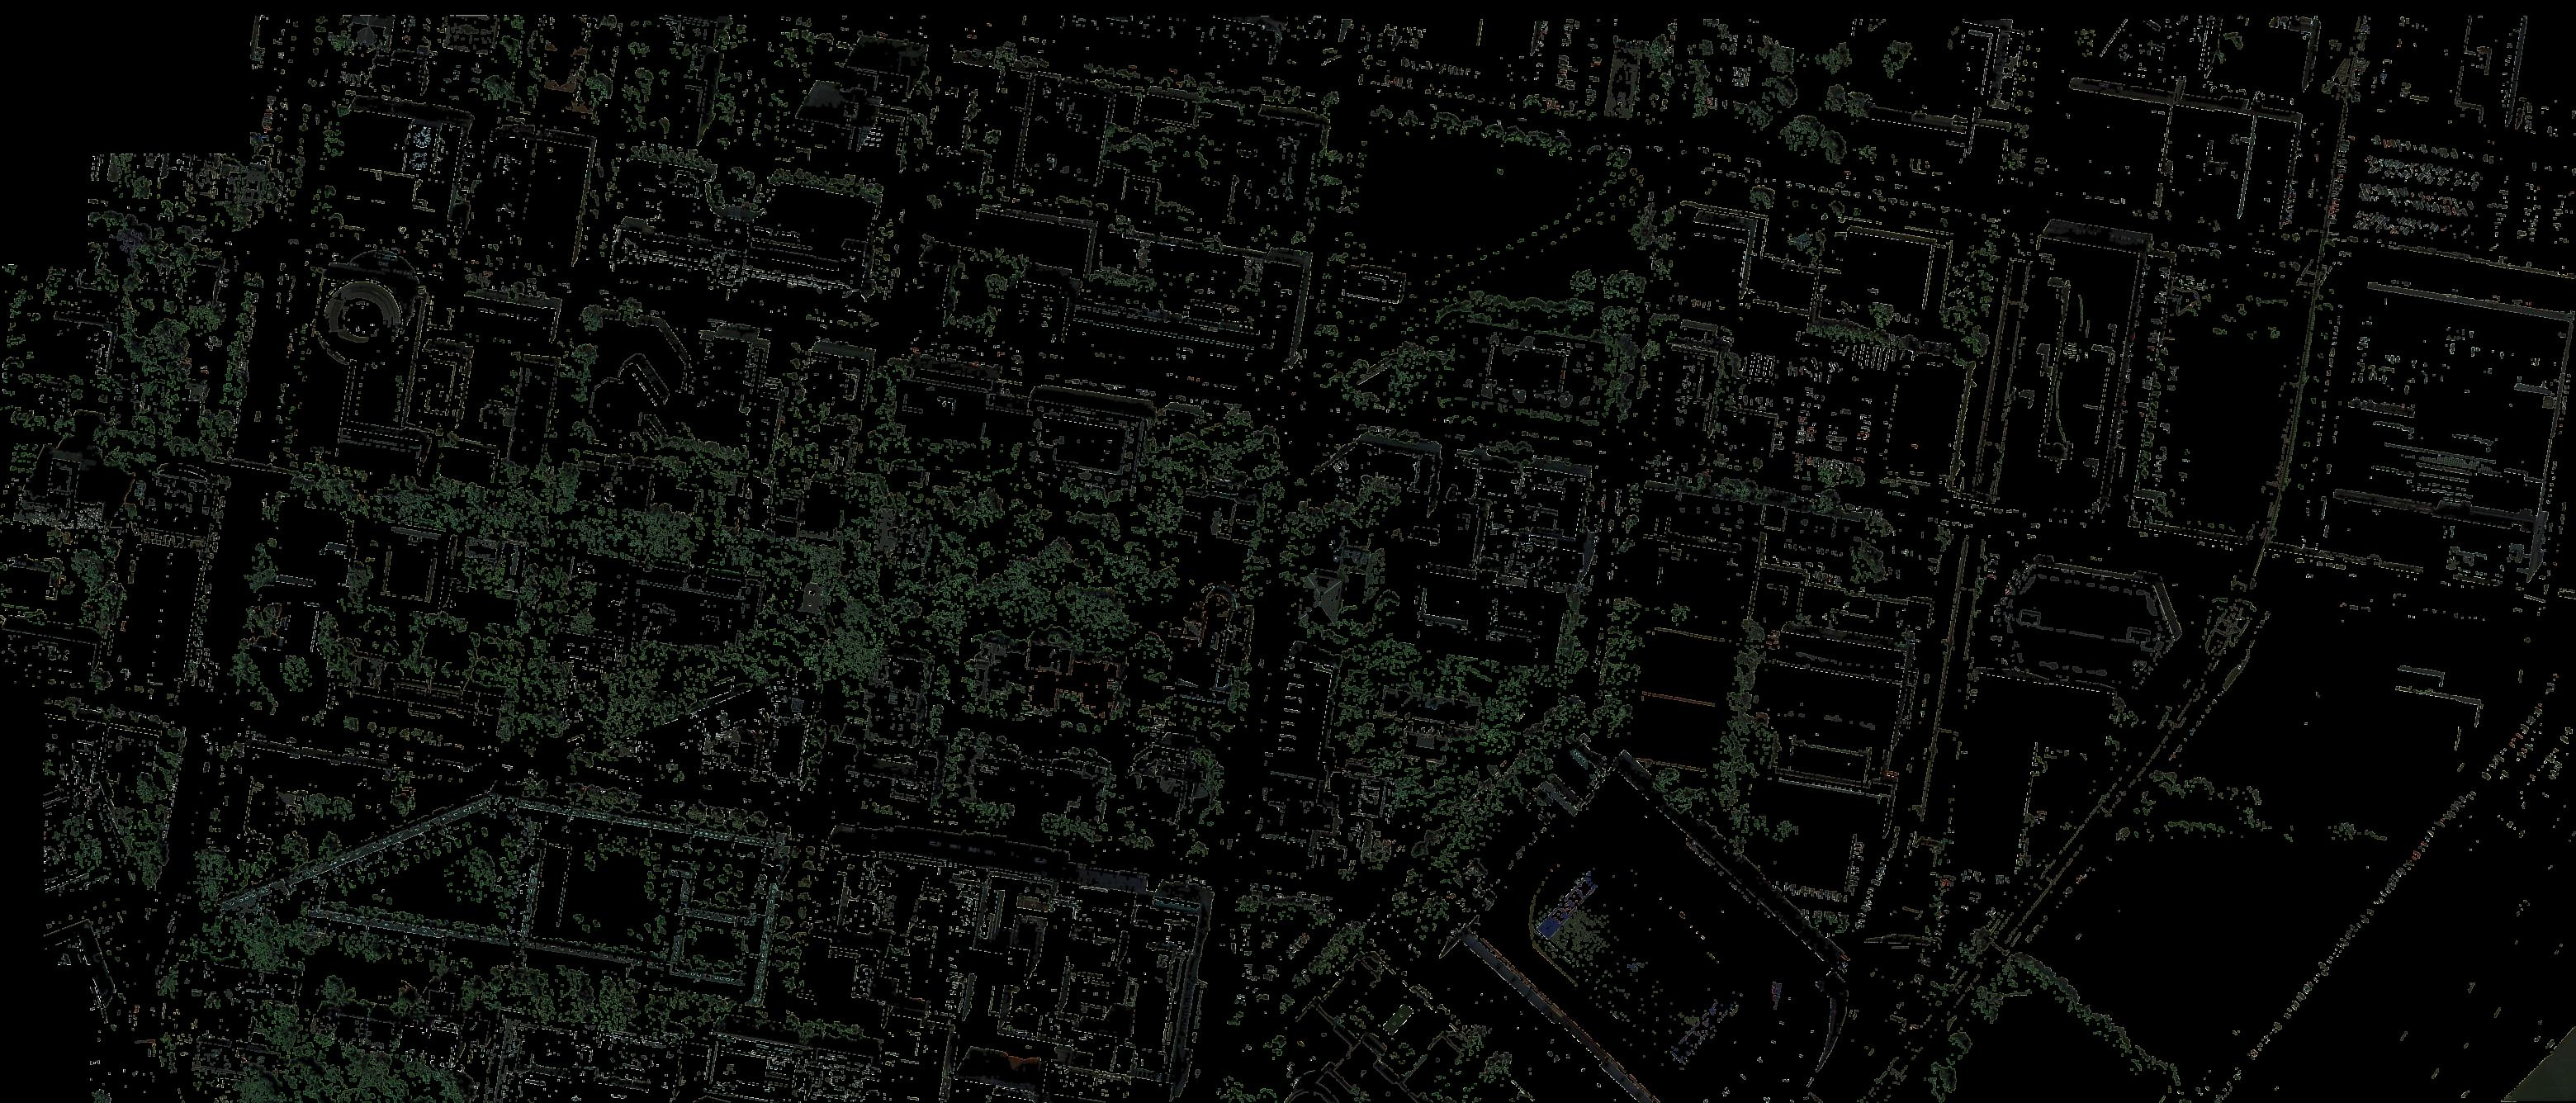
\includegraphics[clip,scale=0.07]{10rgb.jpg} & 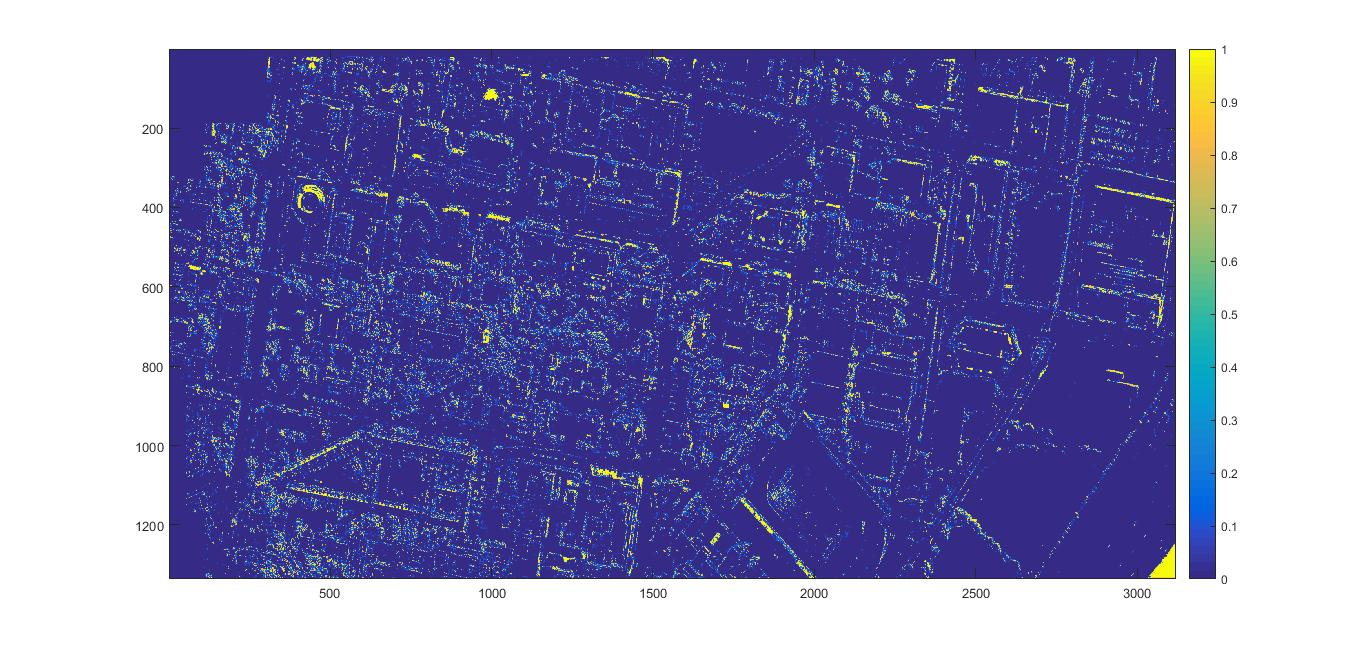
\includegraphics[trim={6cm 2.5cm 4.5cm 1.6cm},clip,scale=0.18]{10.jpg} & \vspace{-3cm}Gaussian Blur \\  
\midrule 
\vspace{-3cm}
\hspace{-0.6cm}
K-means, K = 11 & 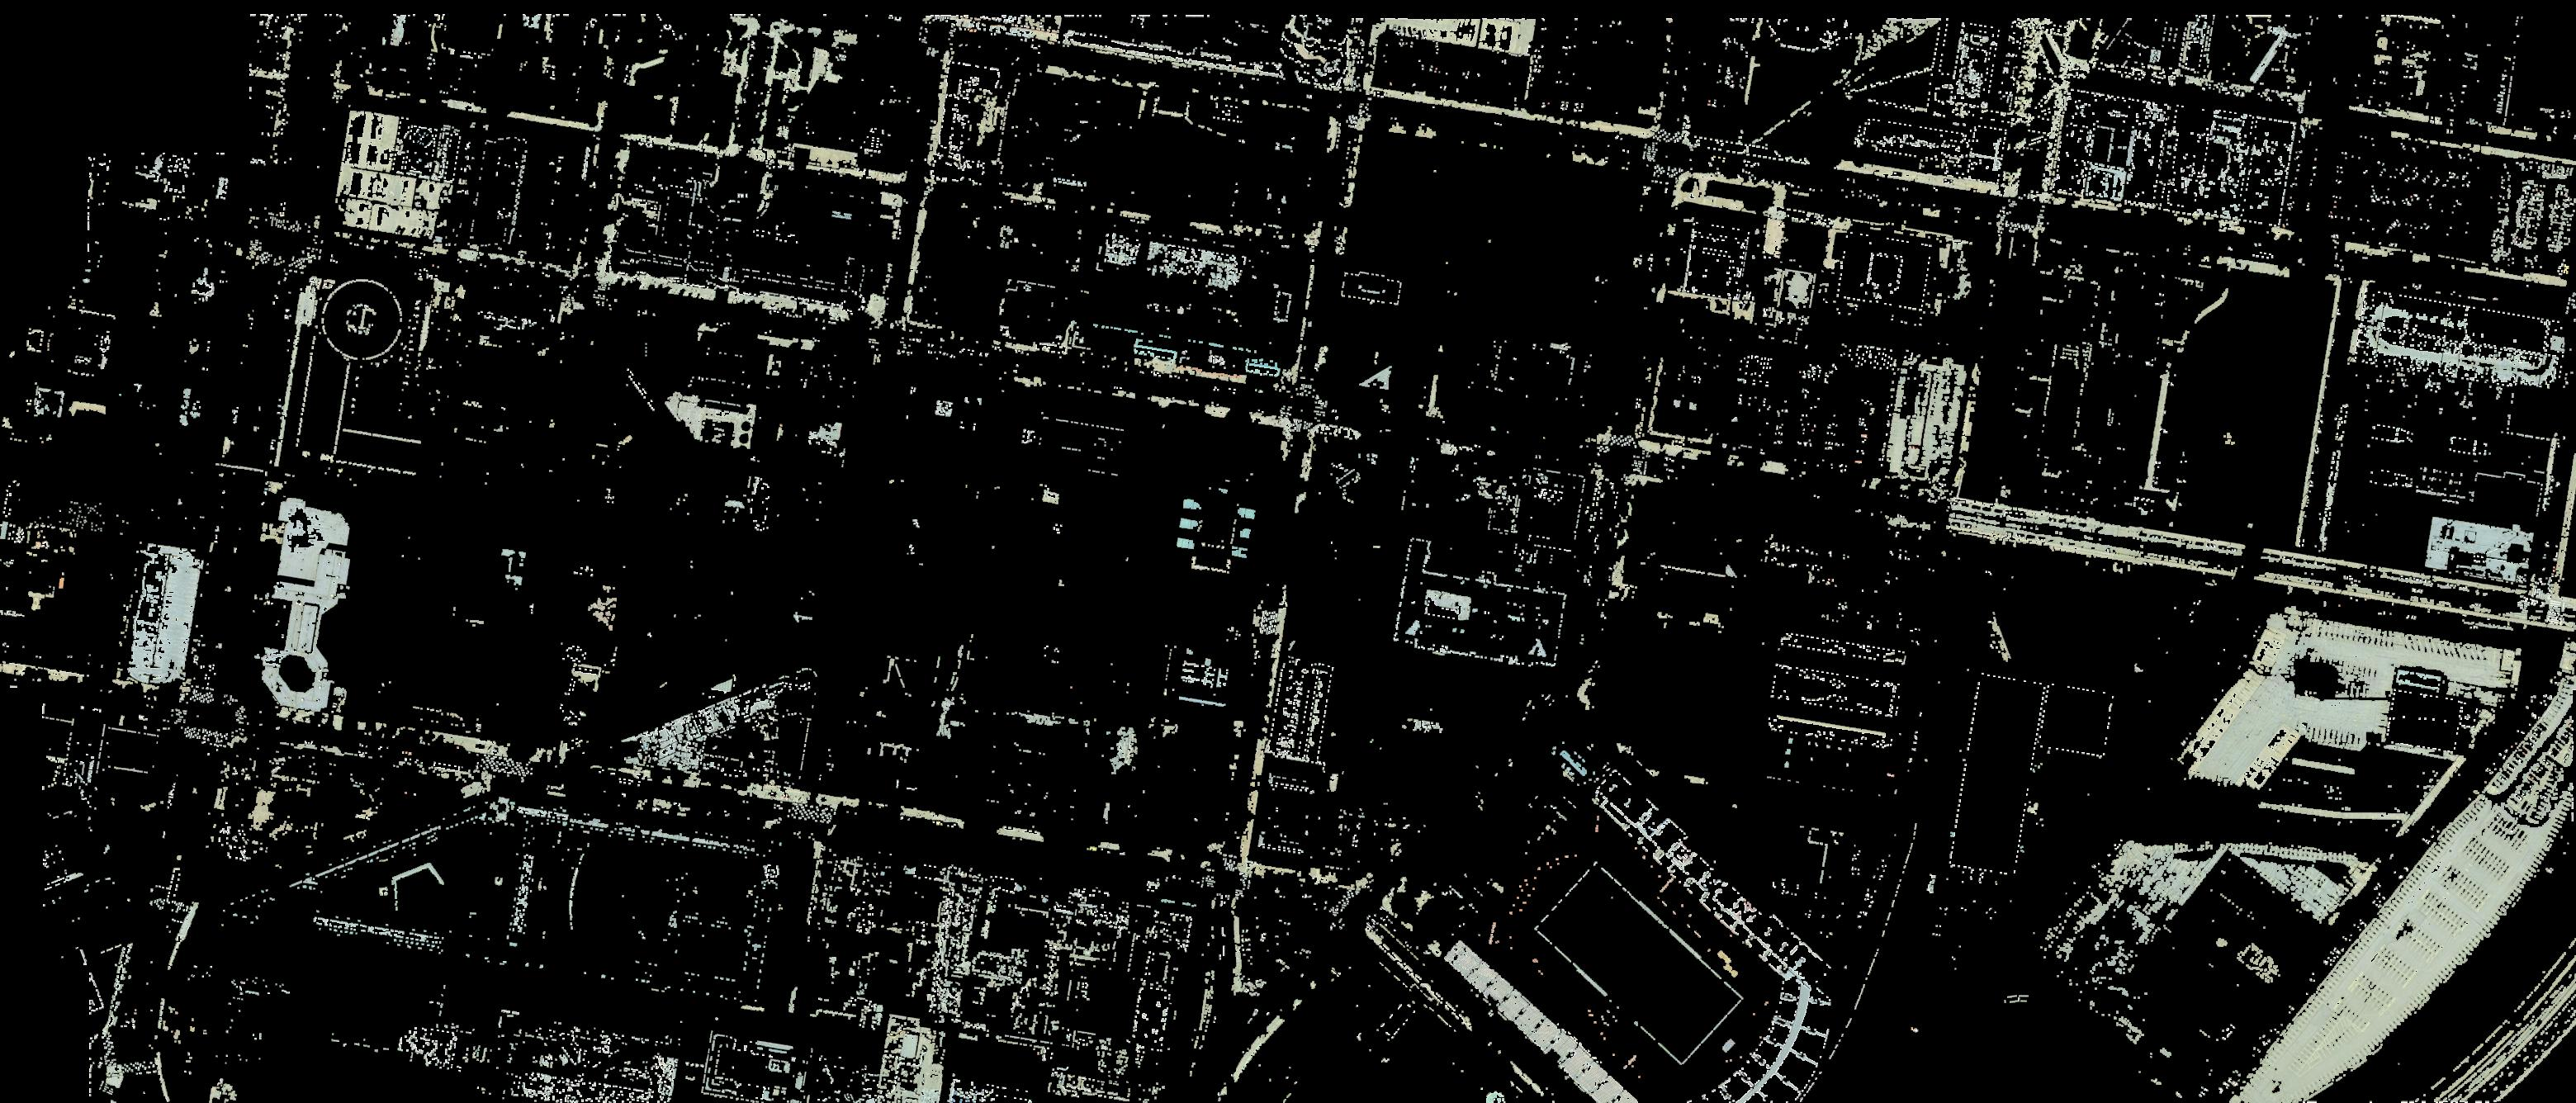
\includegraphics[clip,scale=0.07]{11rgb.jpg} & 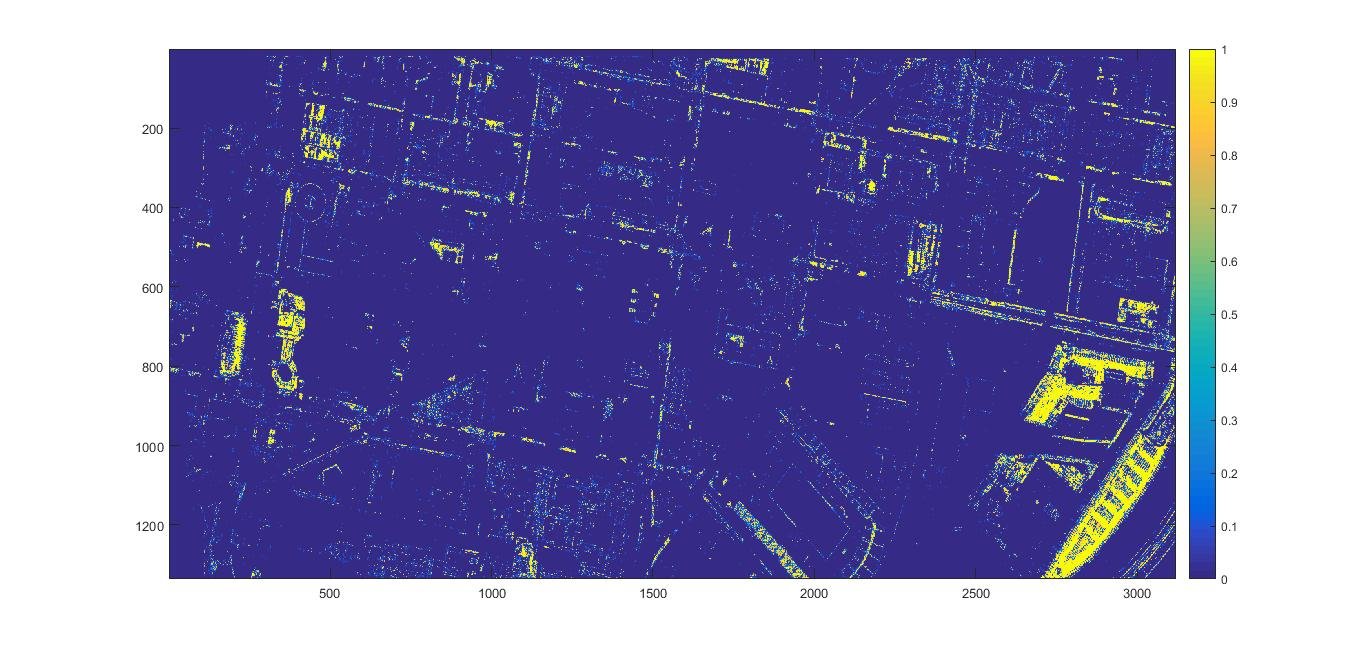
\includegraphics[trim={6cm 2.5cm 4.5cm 1.6cm},clip,scale=0.18]{11.jpg} & \vspace{-3cm}Gaussian Blur \\ 
\midrule
\vspace{-3cm}
\hspace{-0.6cm}
K-means, K = 12 & 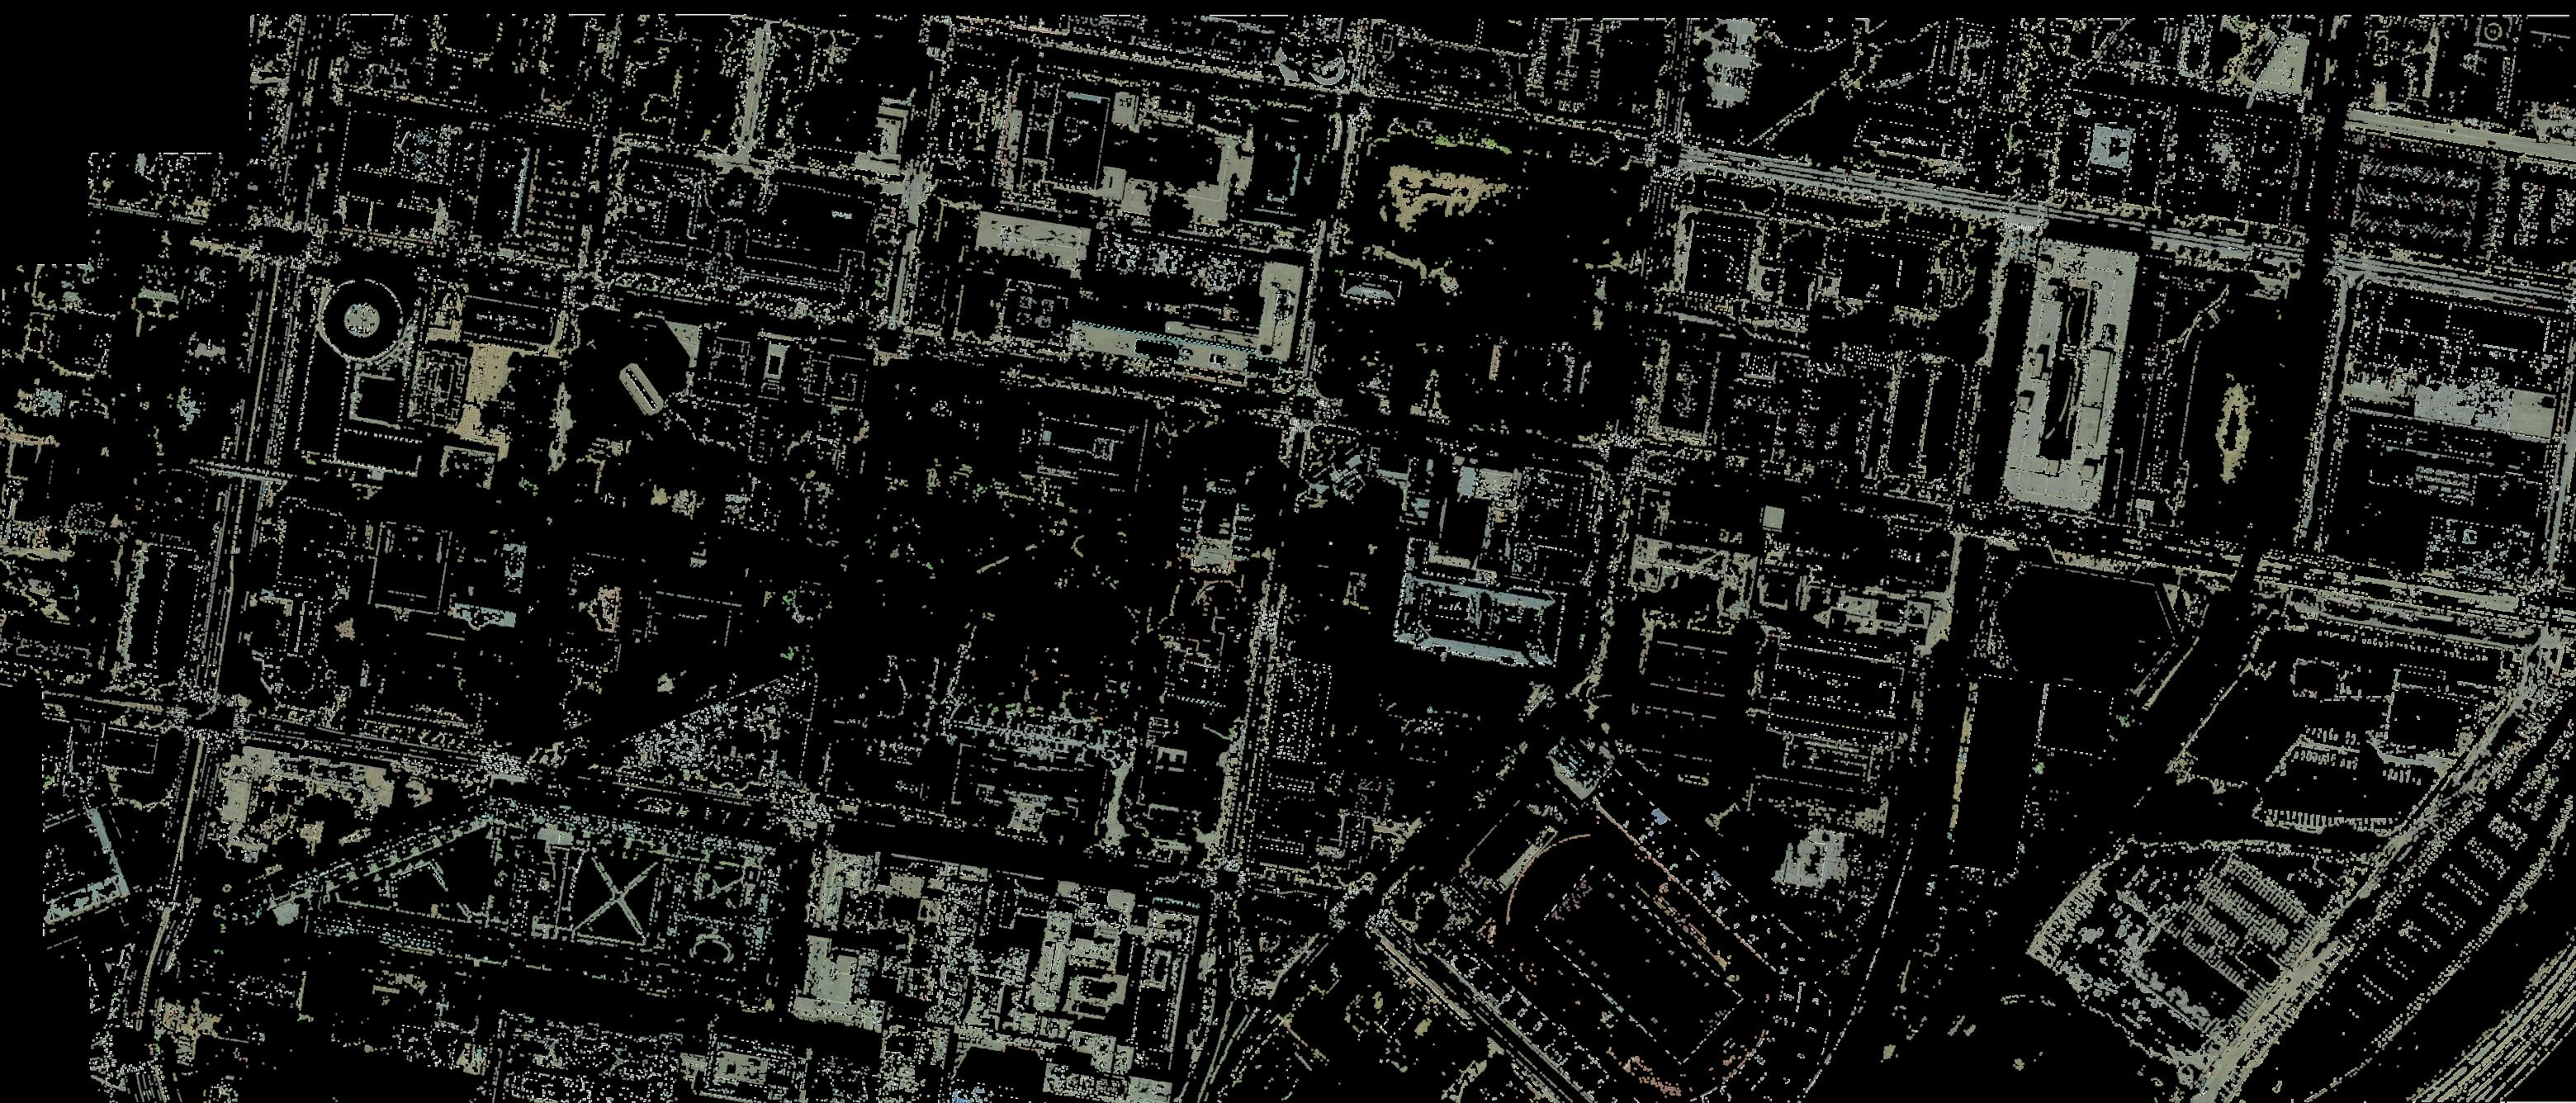
\includegraphics[clip,scale=0.07]{12rgb.jpg} & 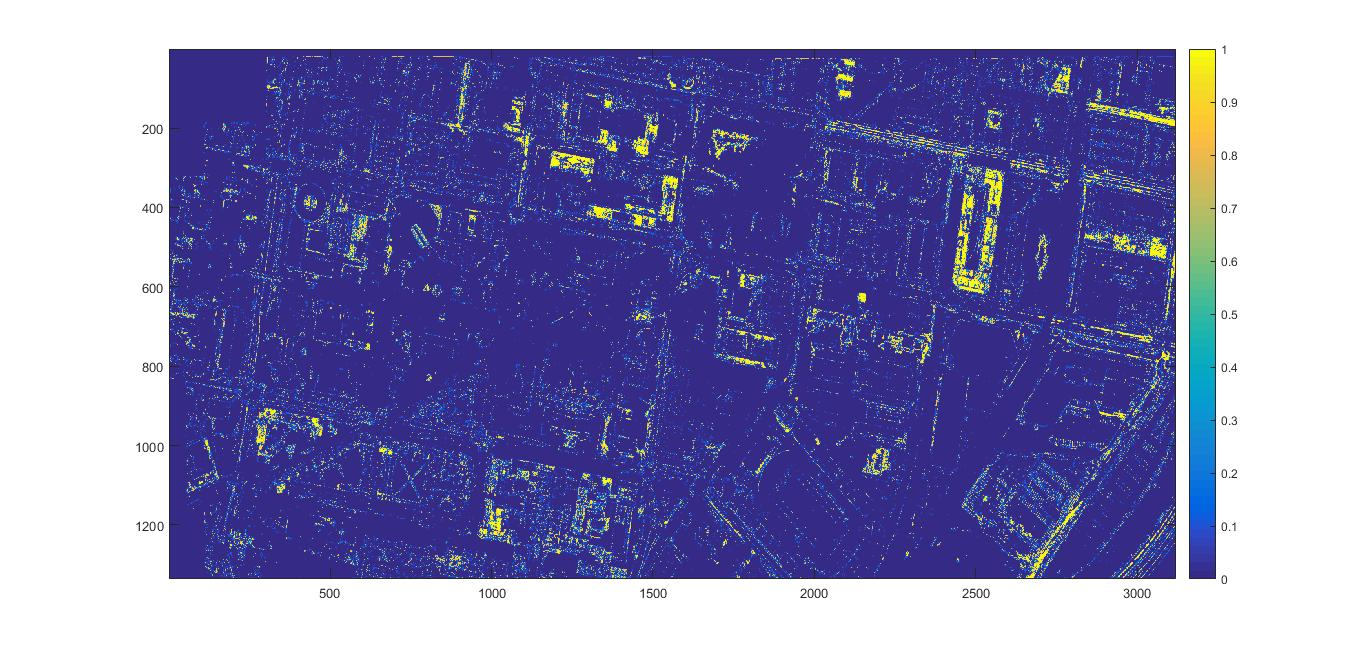
\includegraphics[trim={6cm 2.5cm 4.5cm 1.6cm},clip,scale=0.18]{12.jpg} & \vspace{-3cm}Gaussian Blur \\ 
\bottomrule
\end{tabular} 
\end{table*}

\begin{table*}
\centering
\begin{tabular}{>{\centering\arraybackslash}M{8mm}cc>{\centering\arraybackslash}M{20mm}}
\toprule
Feature & Masked RGB Image & Feature & Post Processing \\ 
\midrule
\vspace{-3cm}
\hspace{-0.6cm}
K-means, K = 13 & 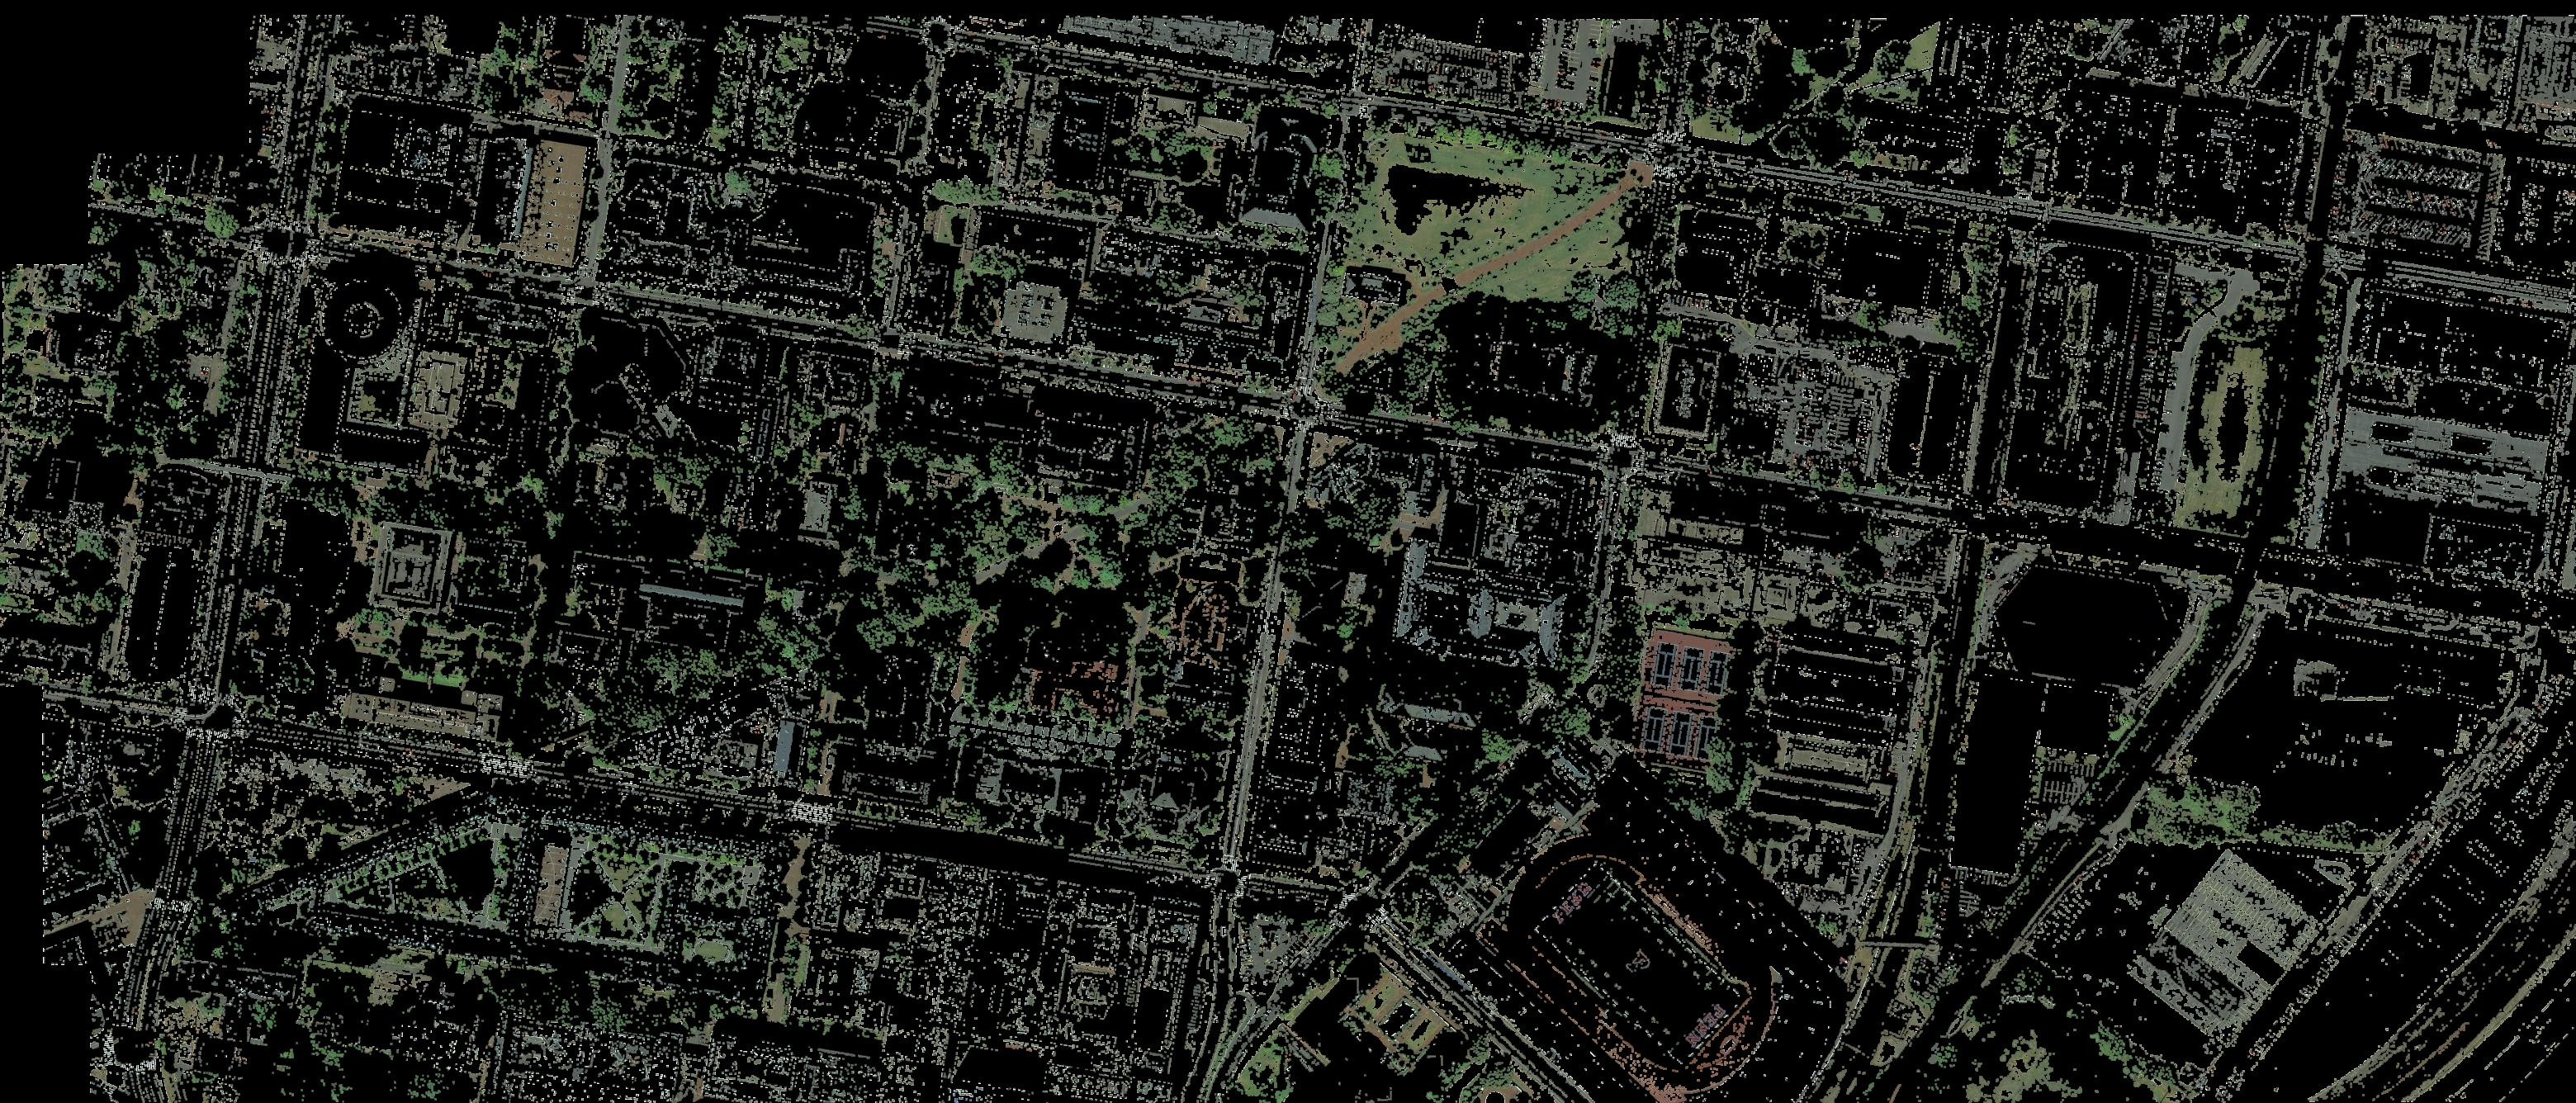
\includegraphics[clip,scale=0.07]{13rgb.jpg} & 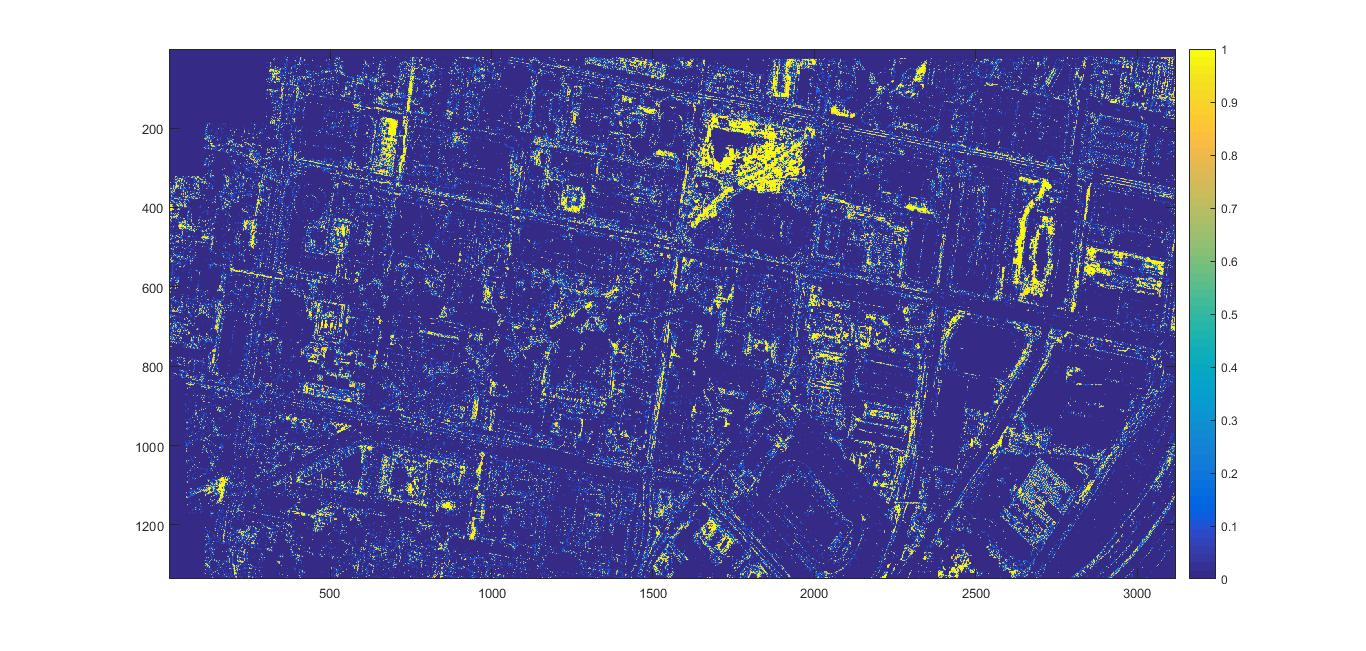
\includegraphics[trim={6cm 2.5cm 4.5cm 1.6cm},clip,scale=0.18]{13.jpg} & \vspace{-3cm}Gaussian Blur \\ 
\midrule 
\vspace{-3cm}
\hspace{-0.6cm}
K-means, K = 14 & 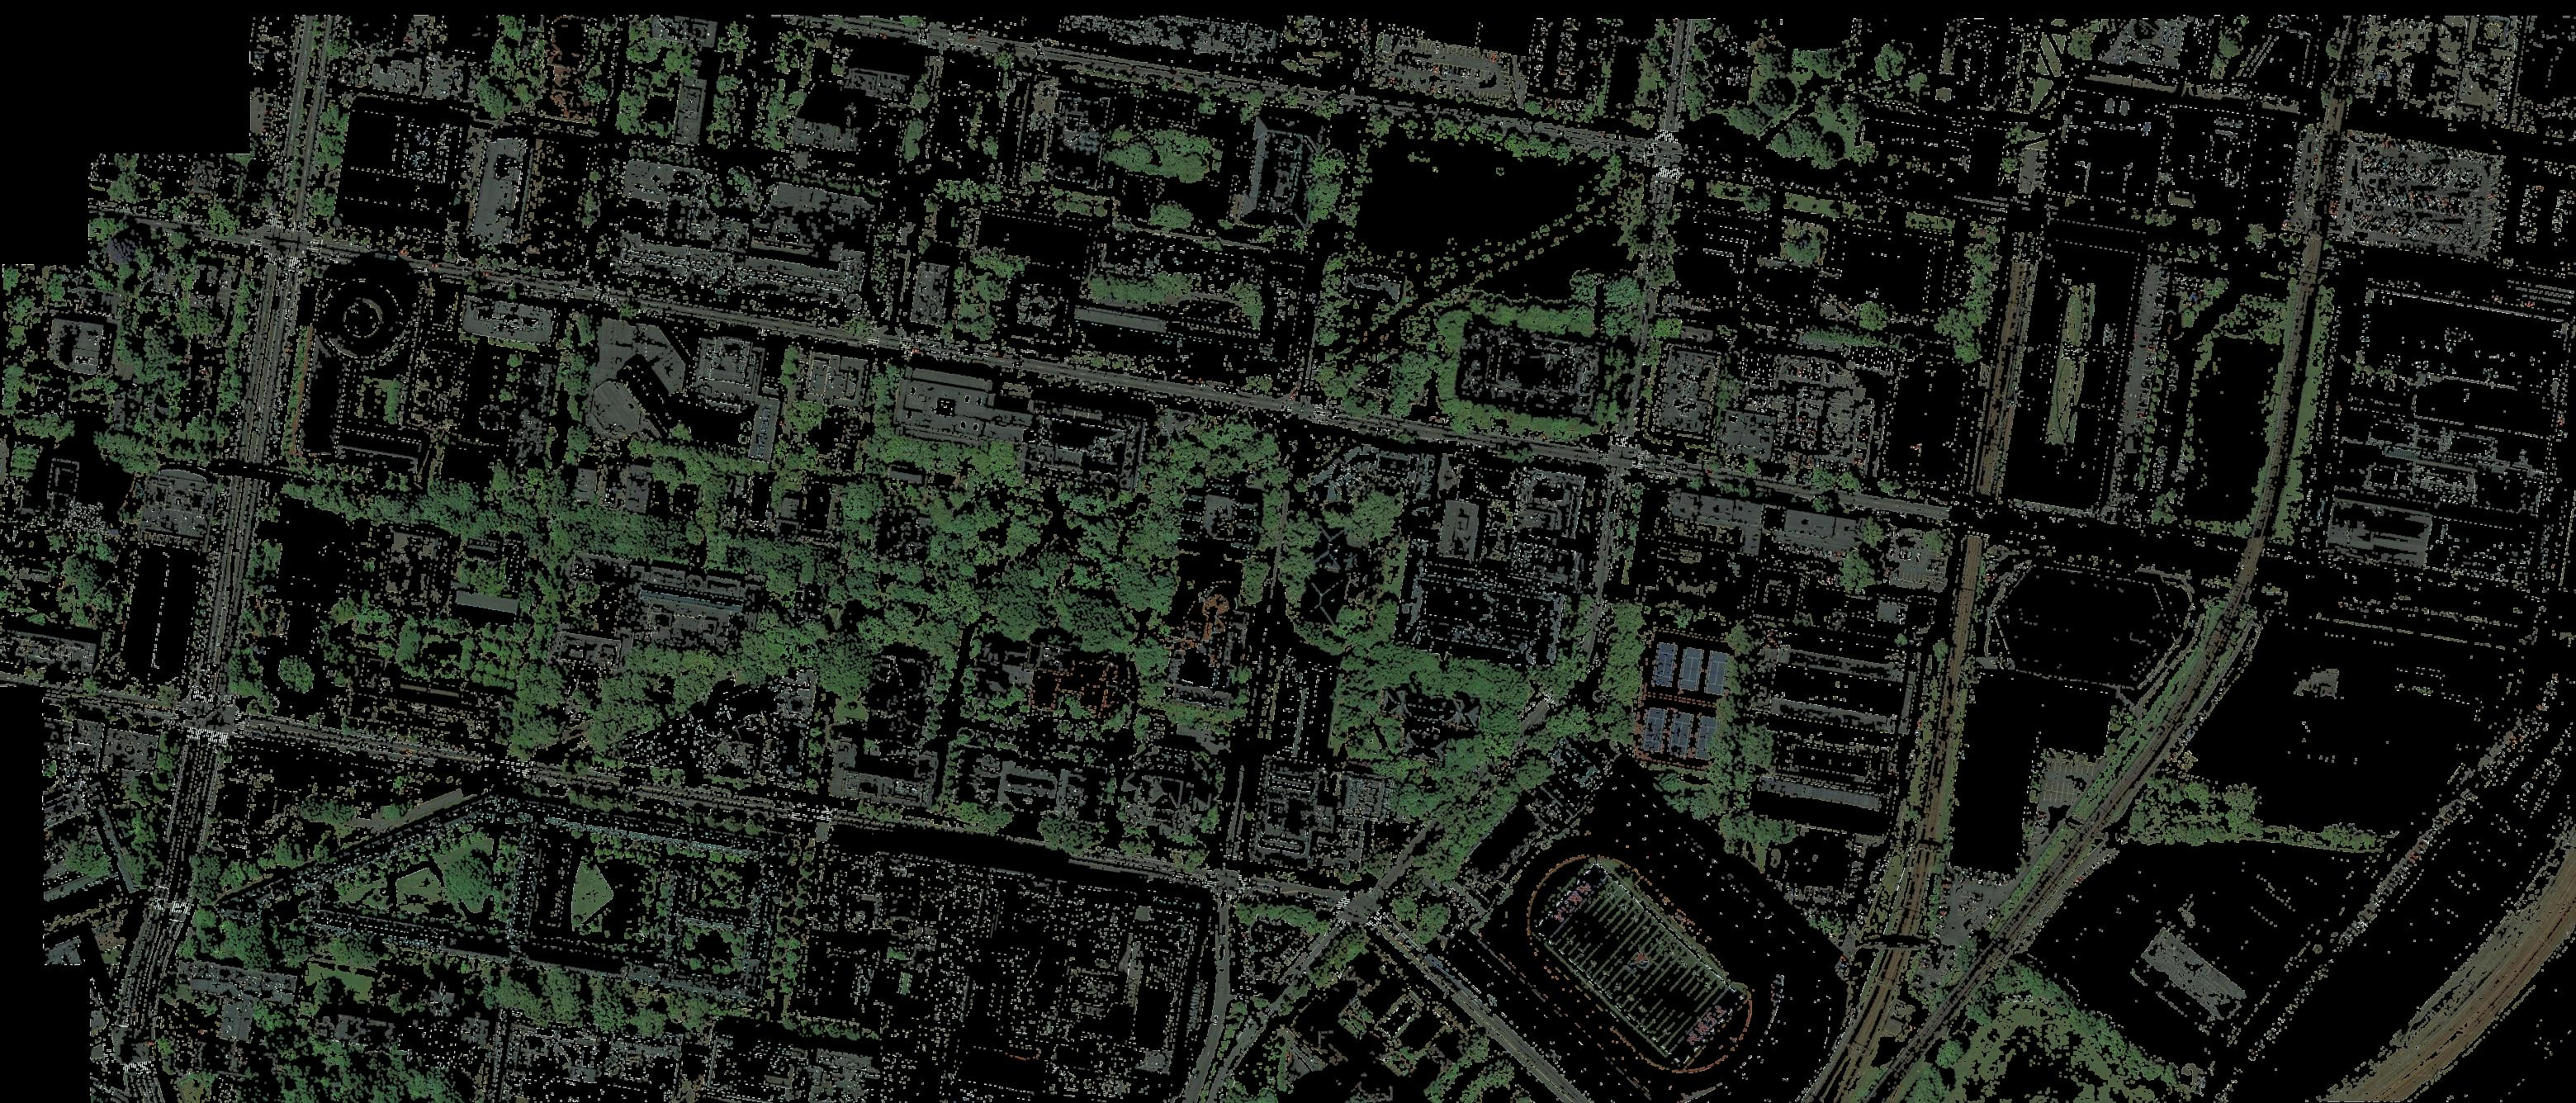
\includegraphics[clip,scale=0.07]{14rgb.jpg} & 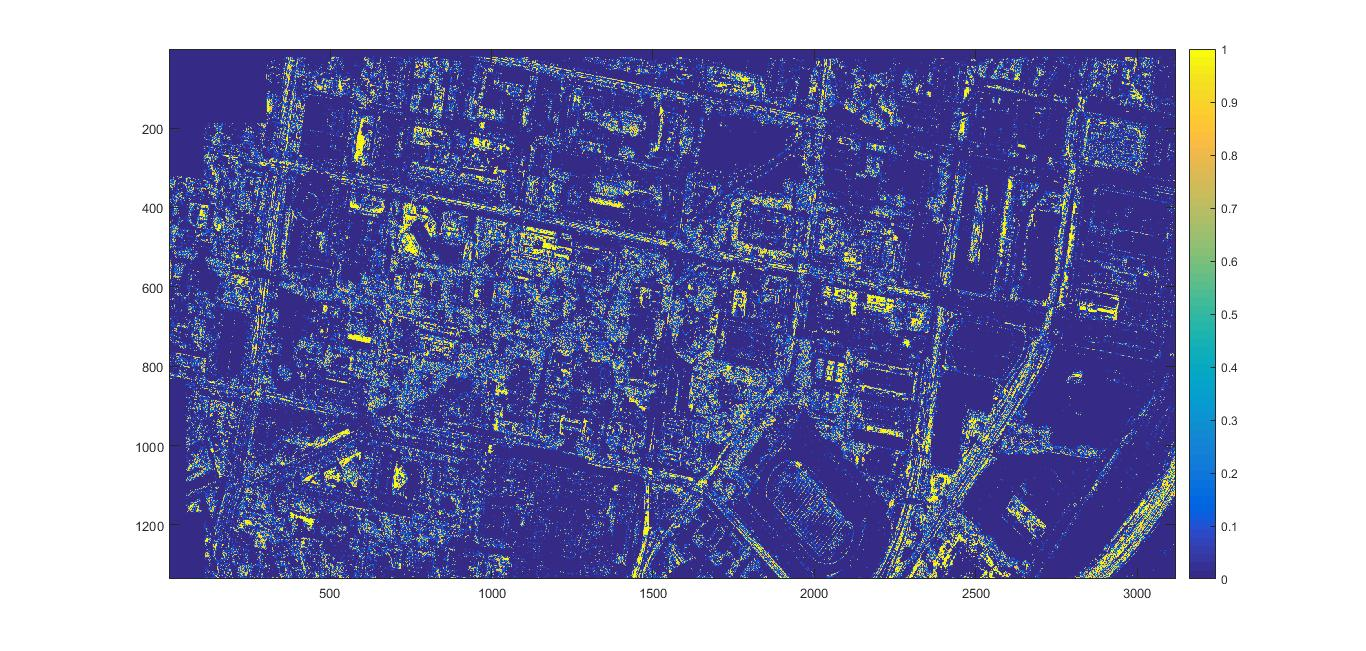
\includegraphics[trim={6cm 2.5cm 4.5cm 1.6cm},clip,scale=0.18]{14.jpg} & \vspace{-3cm}Gaussian Blur \\ 
\midrule 
\vspace{-3cm}
\hspace{-0.6cm}
K-means, K = 15 & 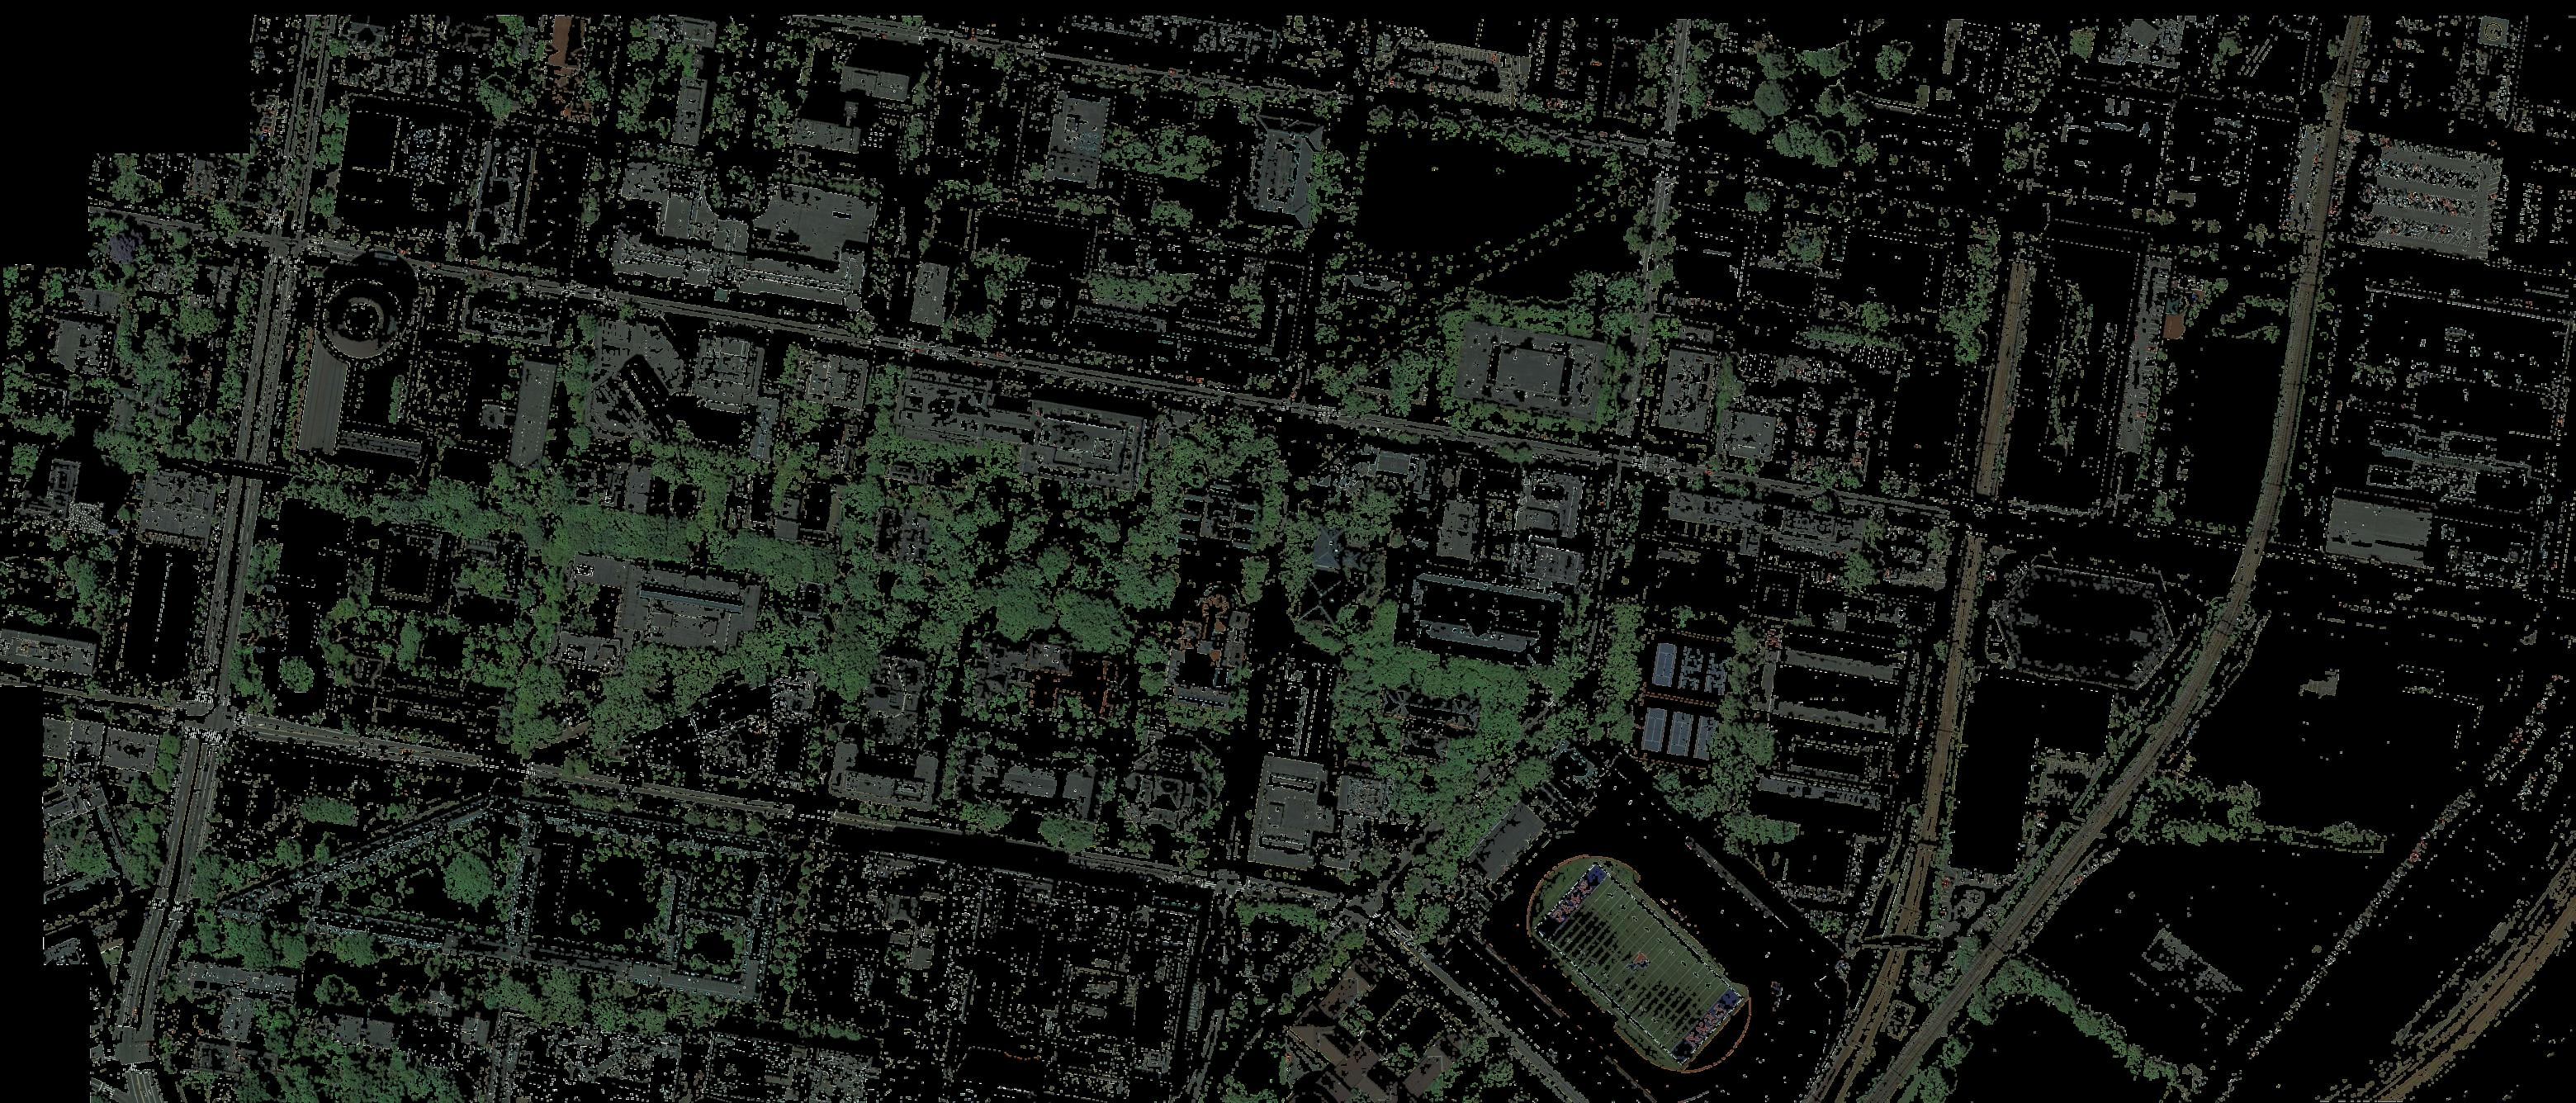
\includegraphics[clip,scale=0.07]{15rgb.jpg} & 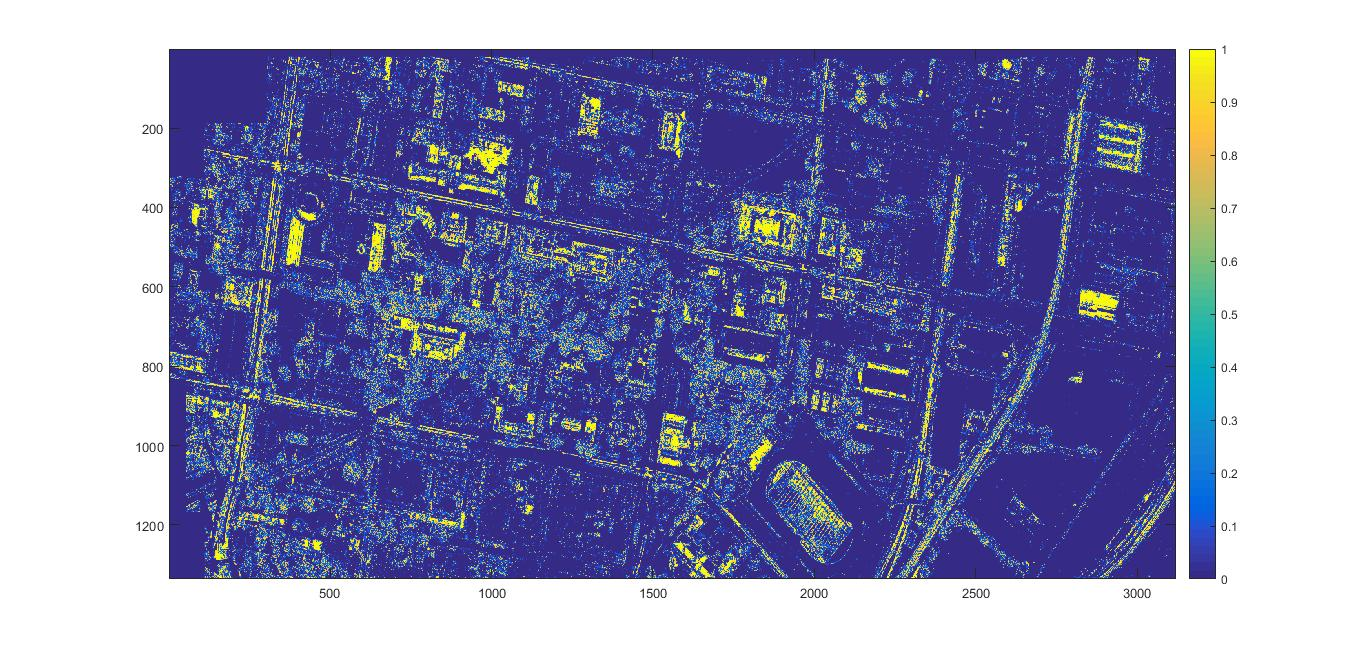
\includegraphics[trim={6cm 2.5cm 4.5cm 1.6cm},clip,scale=0.18]{15.jpg} & \vspace{-3cm}Gaussian Blur \\ 
\midrule 
\vspace{-3cm}
\hspace{-0.6cm}
K-means, K = 16 & 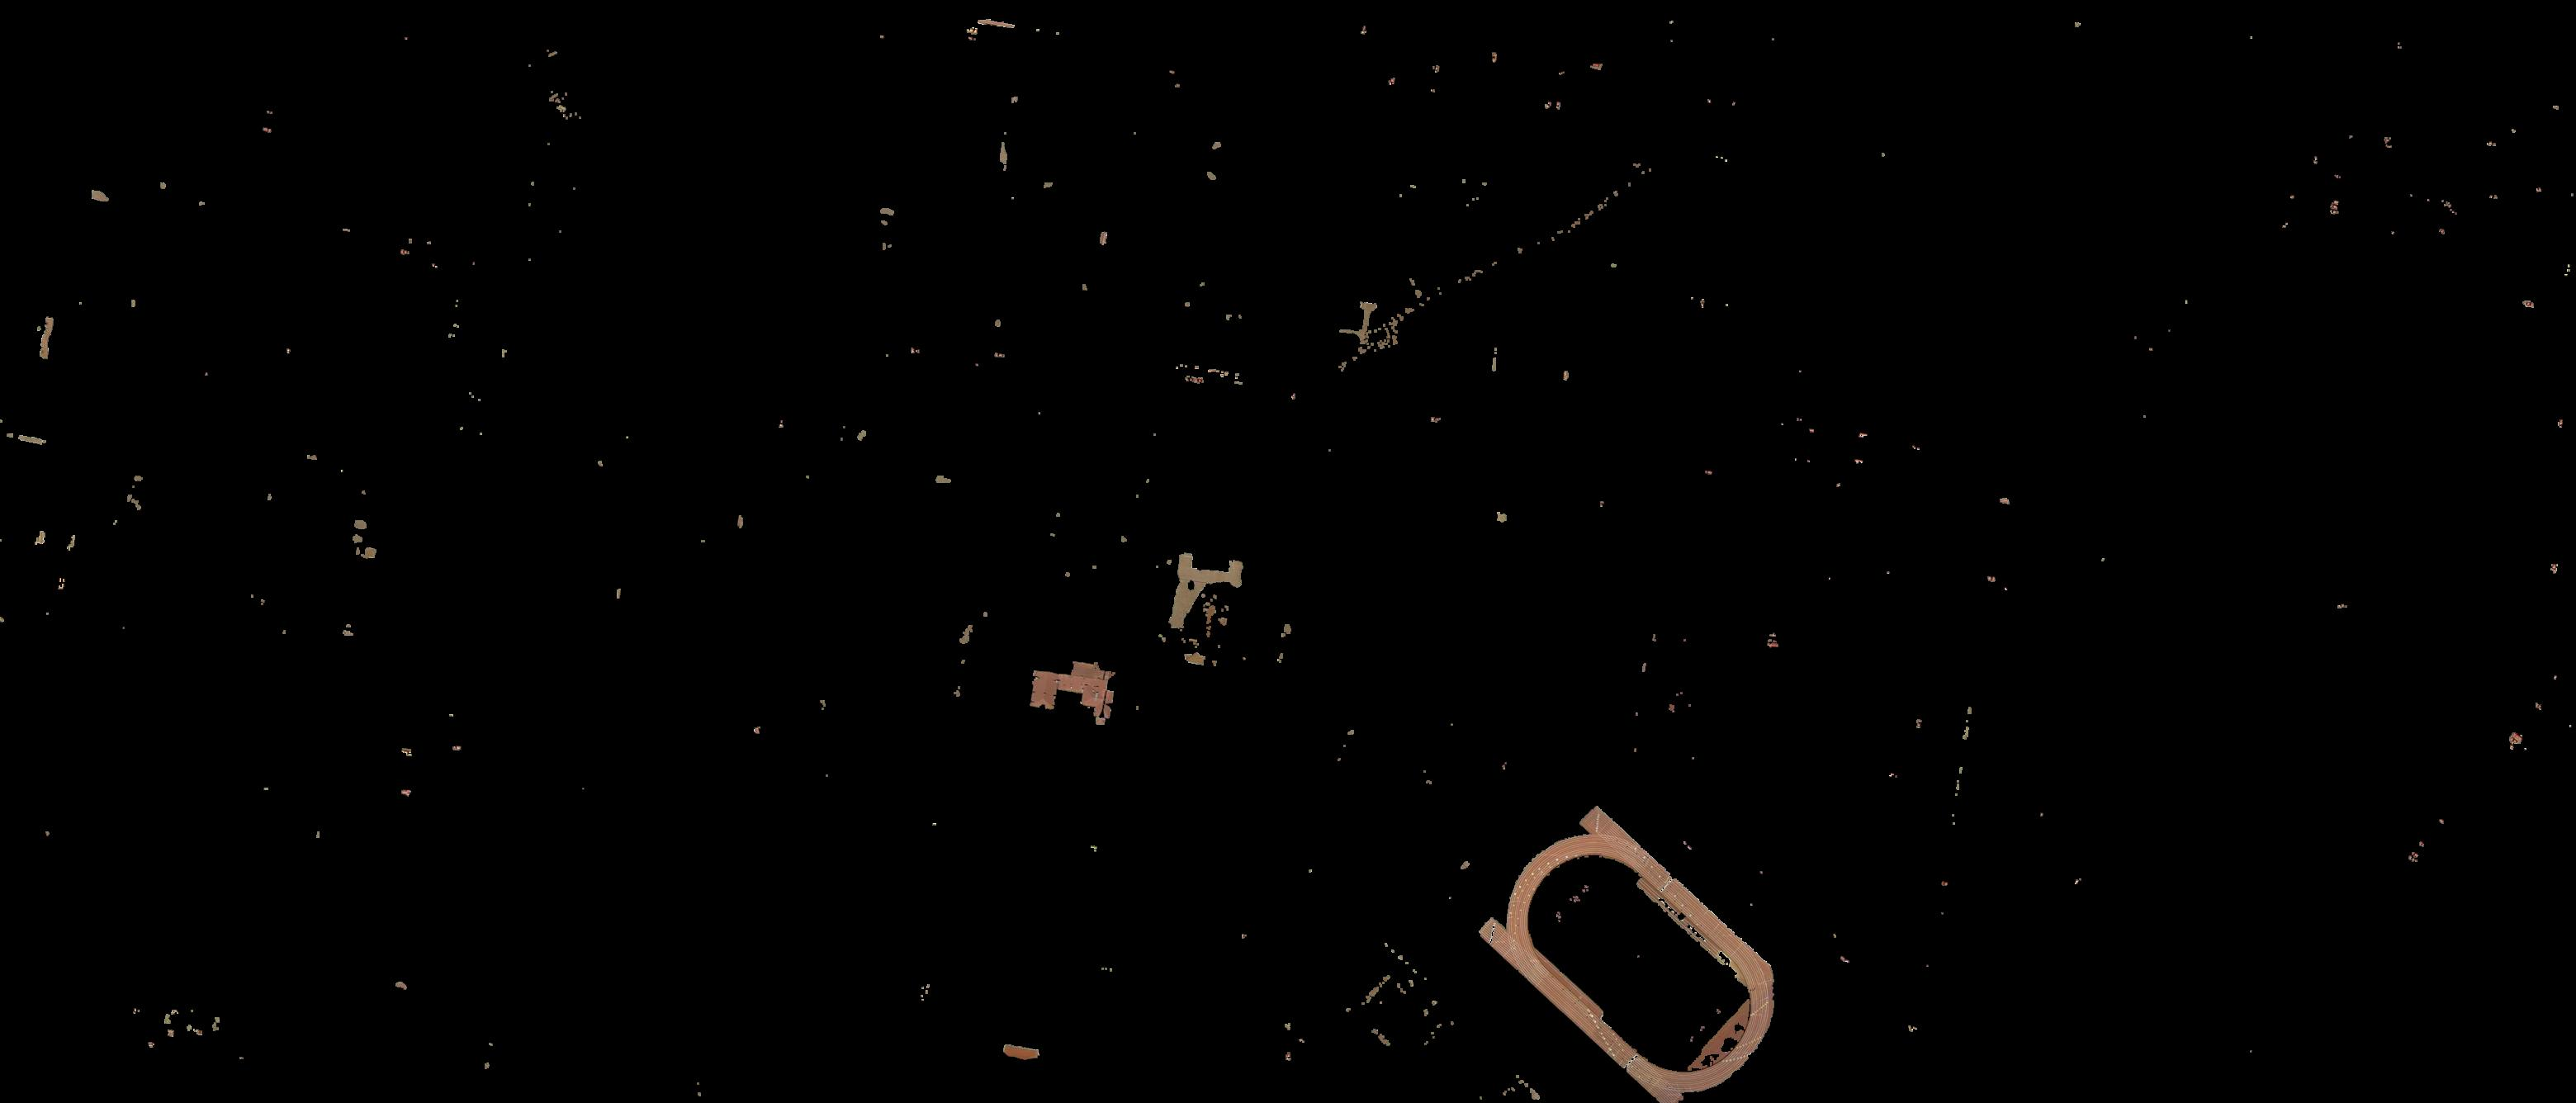
\includegraphics[clip,scale=0.07]{16rgb.jpg} & 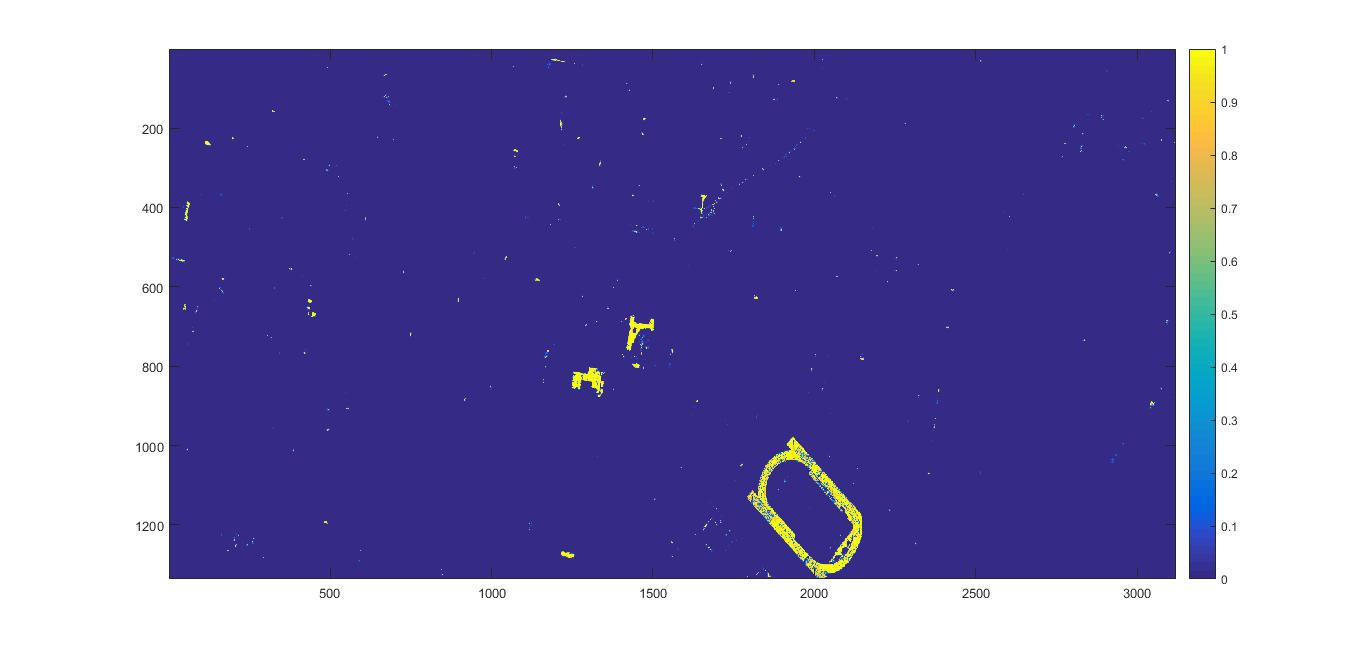
\includegraphics[trim={6cm 2.5cm 4.5cm 1.6cm},clip,scale=0.18]{16.jpg} & \vspace{-3cm}Gaussian Blur \\ 
\midrule 
\vspace{-3cm}
\hspace{-0.3cm}
Black roof & 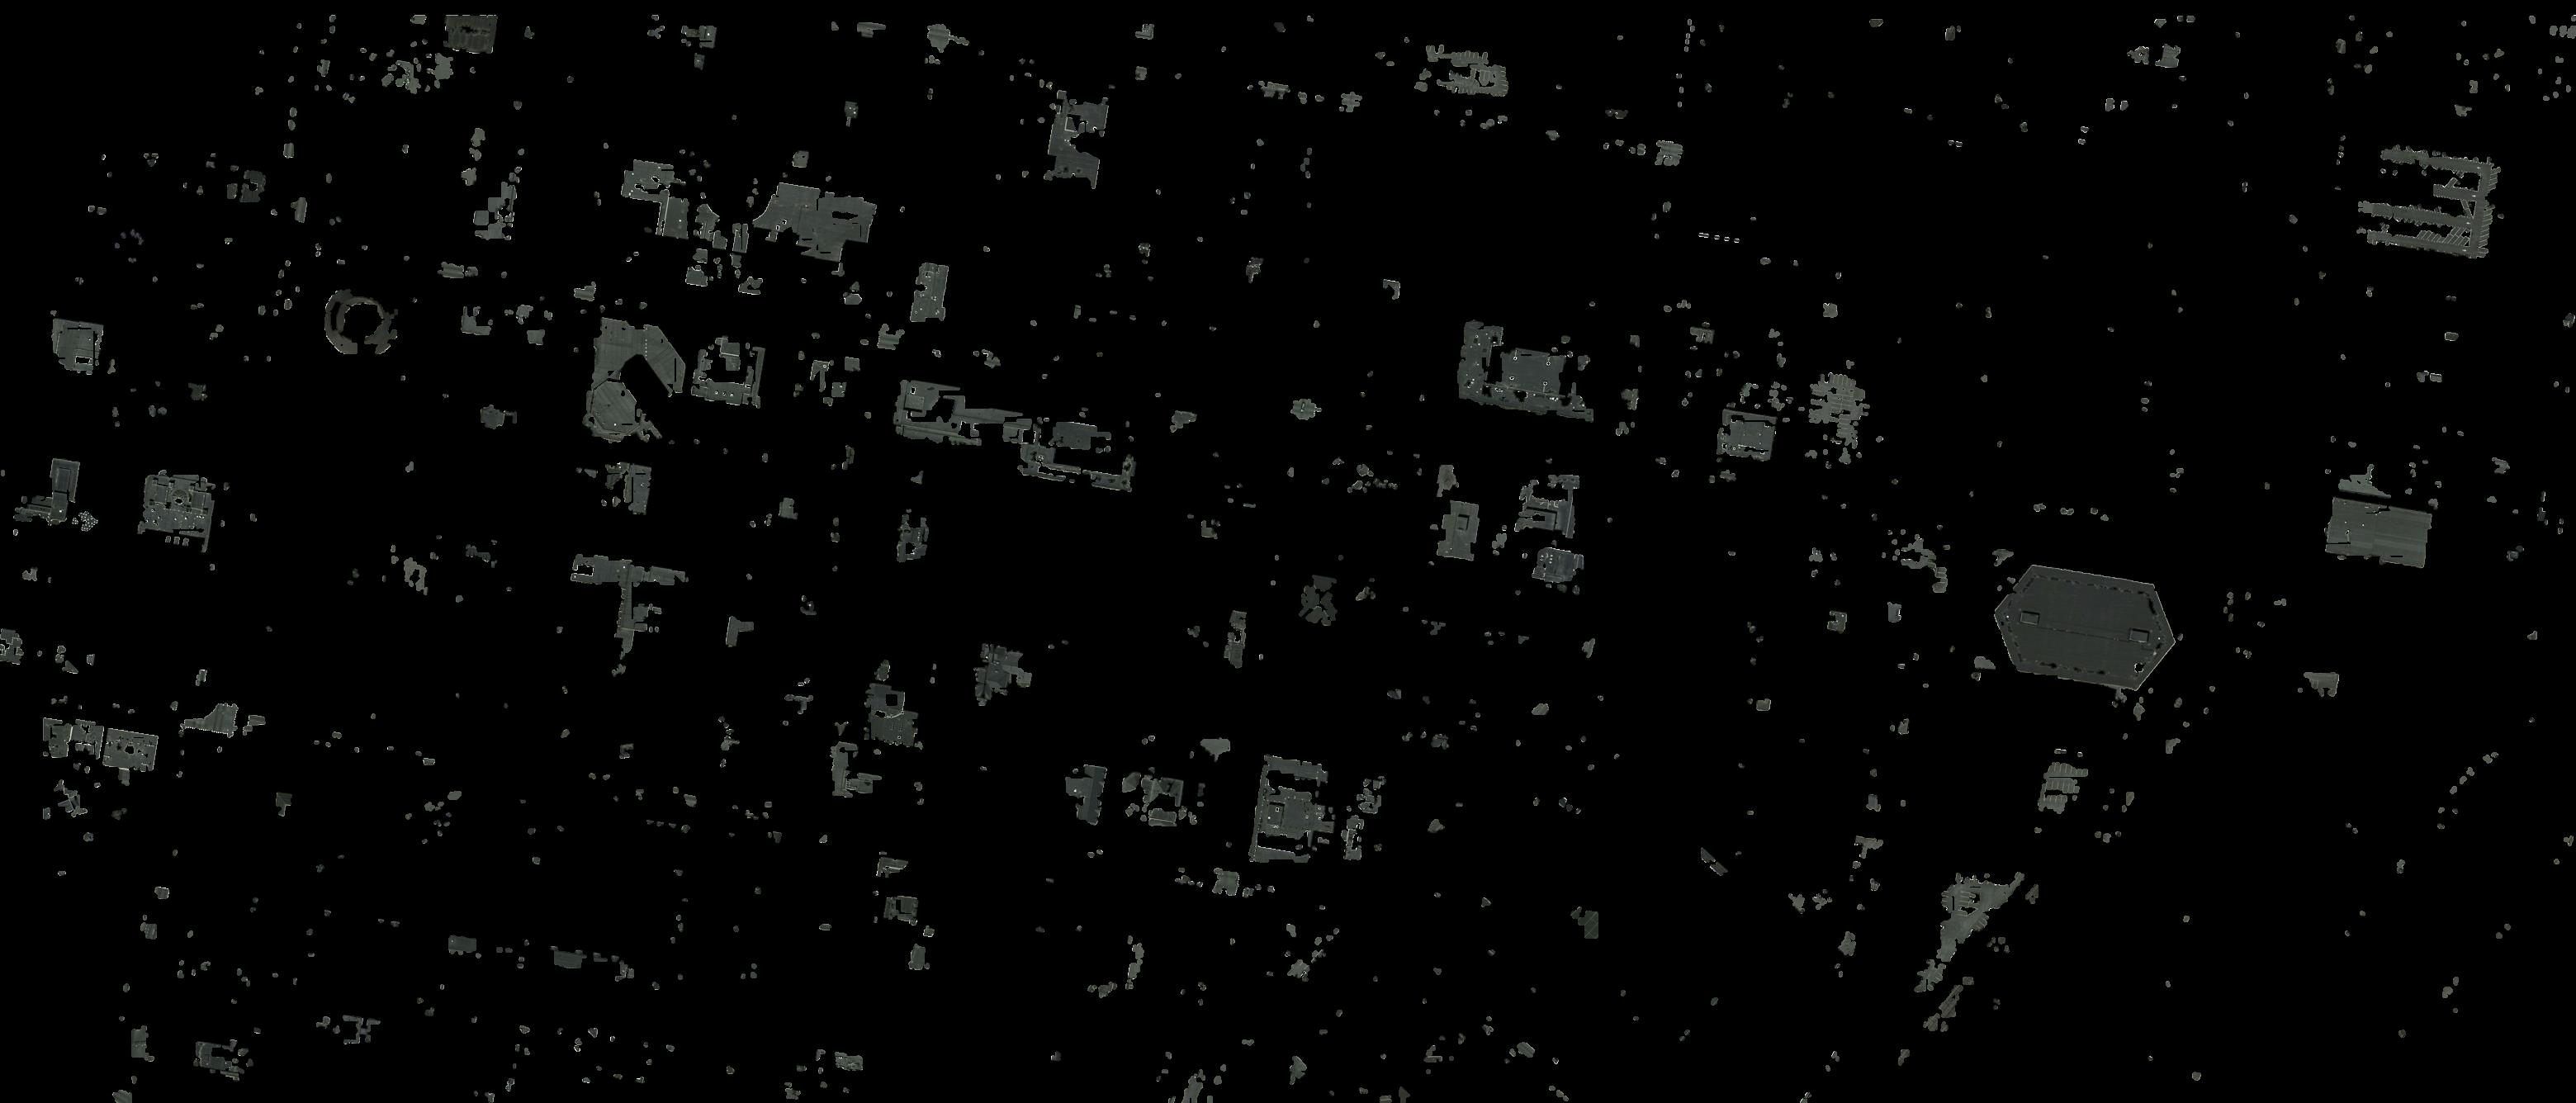
\includegraphics[clip,scale=0.07]{17rgb.jpg} & 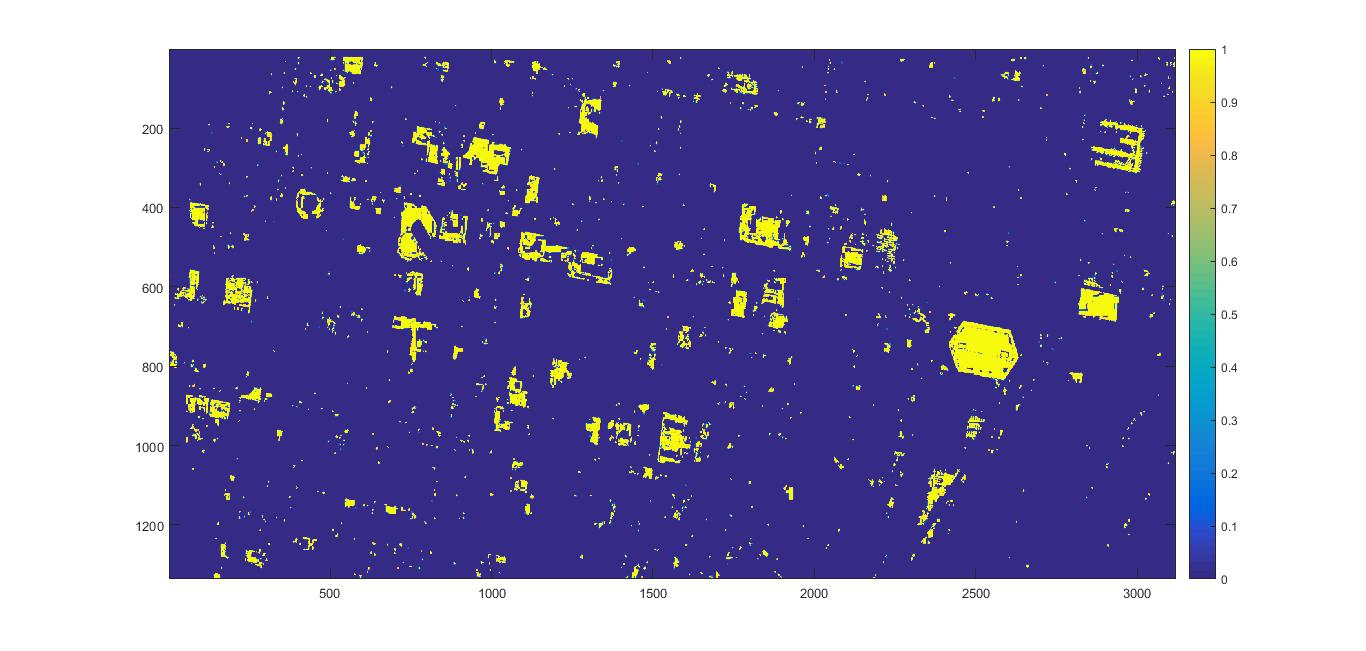
\includegraphics[trim={6cm 2.5cm 4.5cm 1.6cm},clip,scale=0.18]{17.jpg} & \vspace{-3cm} YCbCr, Gaussian Blur, morphological operations, eccentricity \\ 
\midrule 
\vspace{-3cm}
\hspace{-0.4cm}
Brown roof & 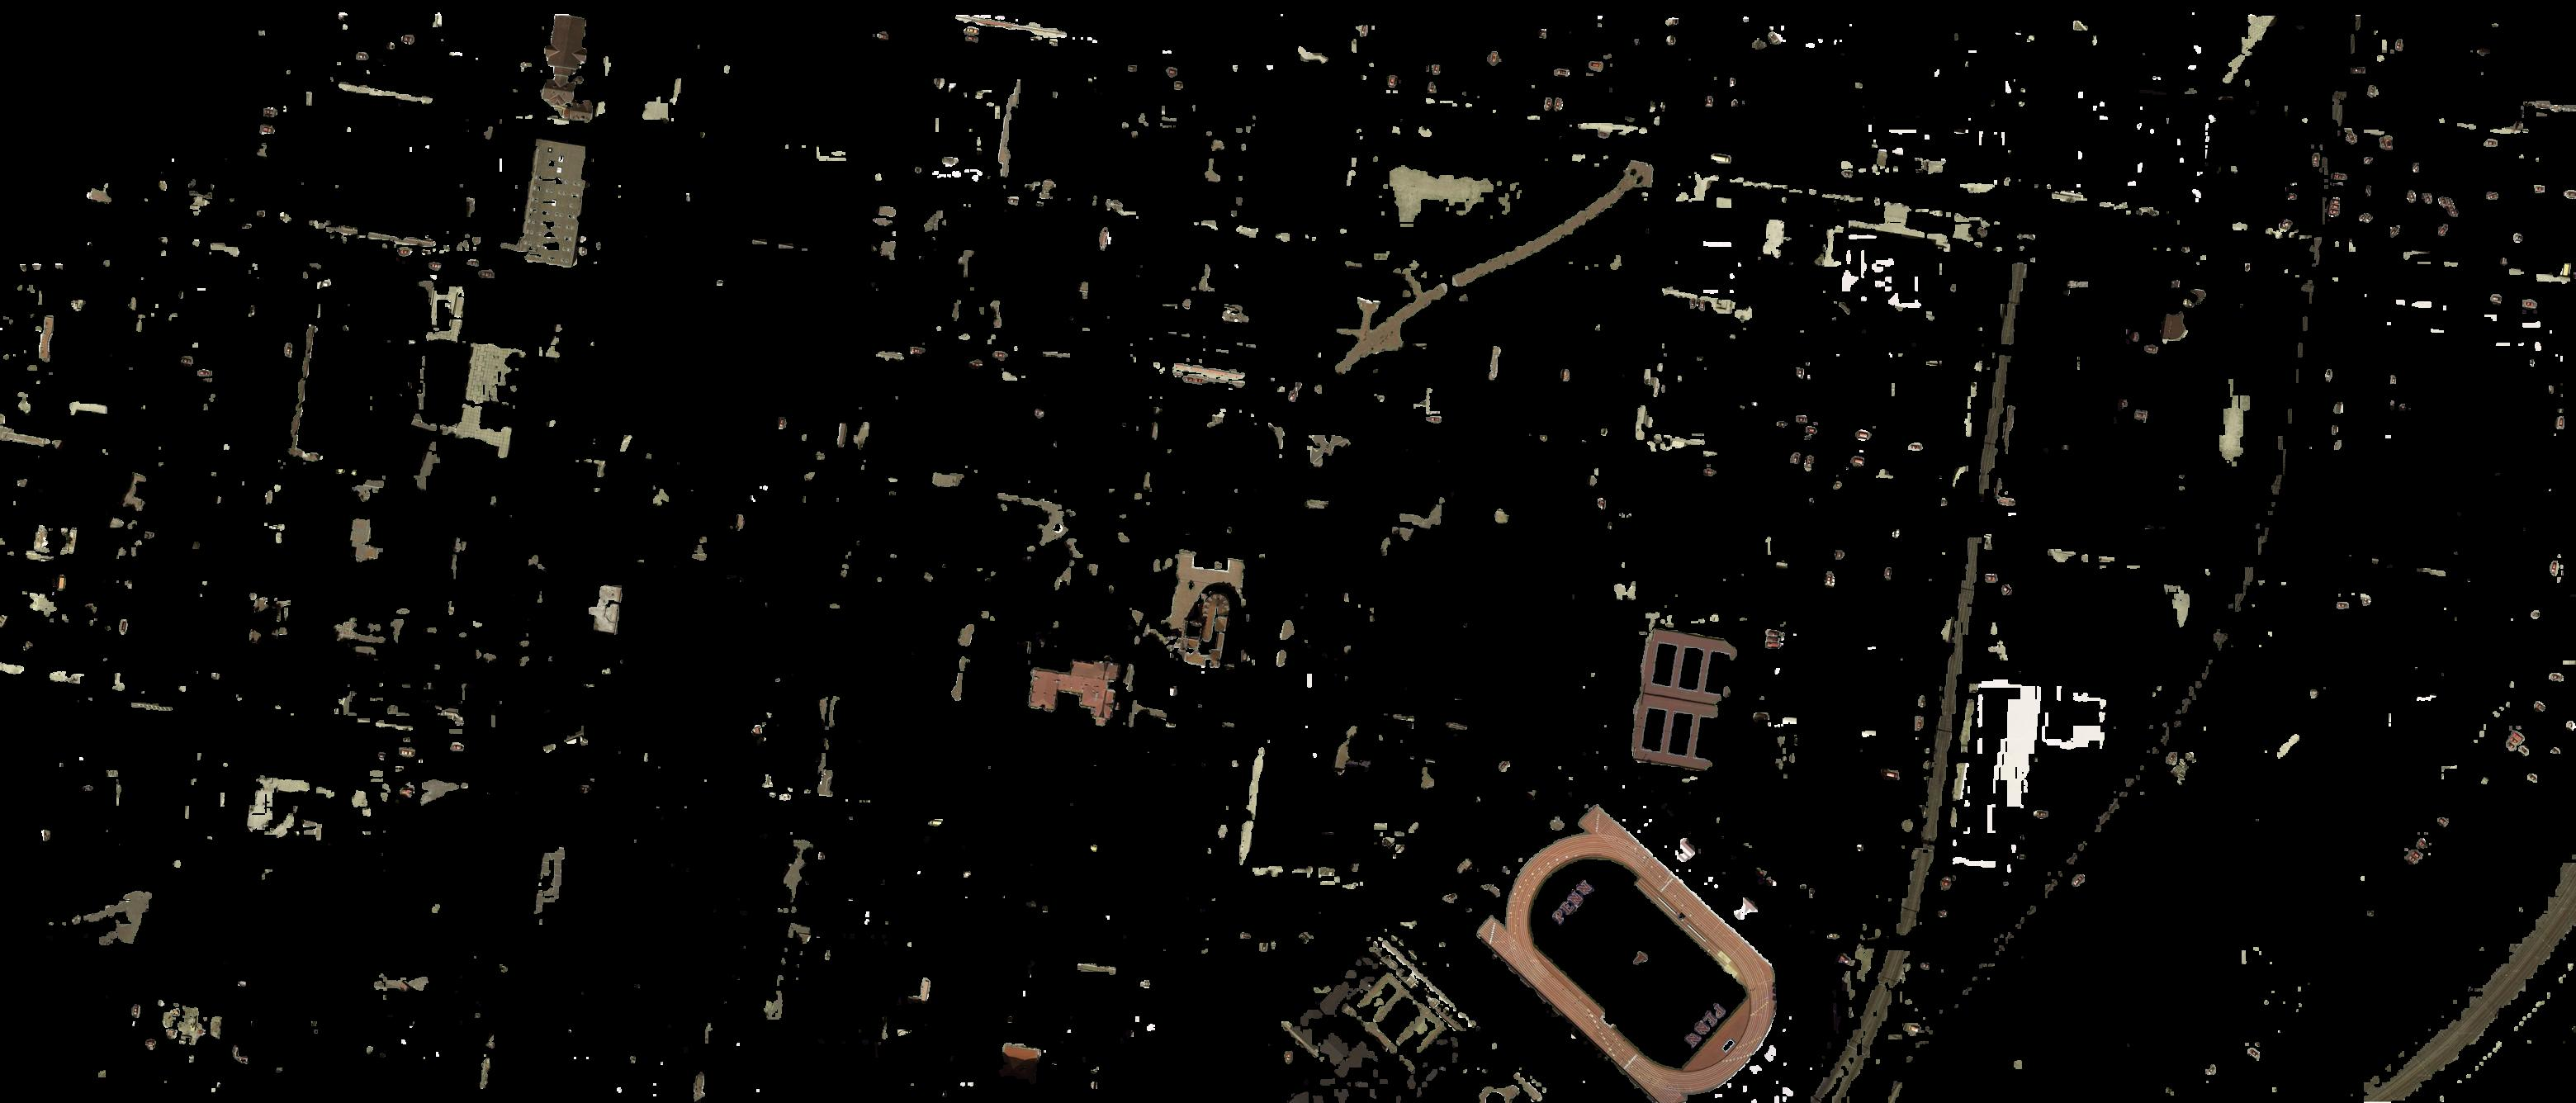
\includegraphics[clip,scale=0.07]{18rgb.jpg} & 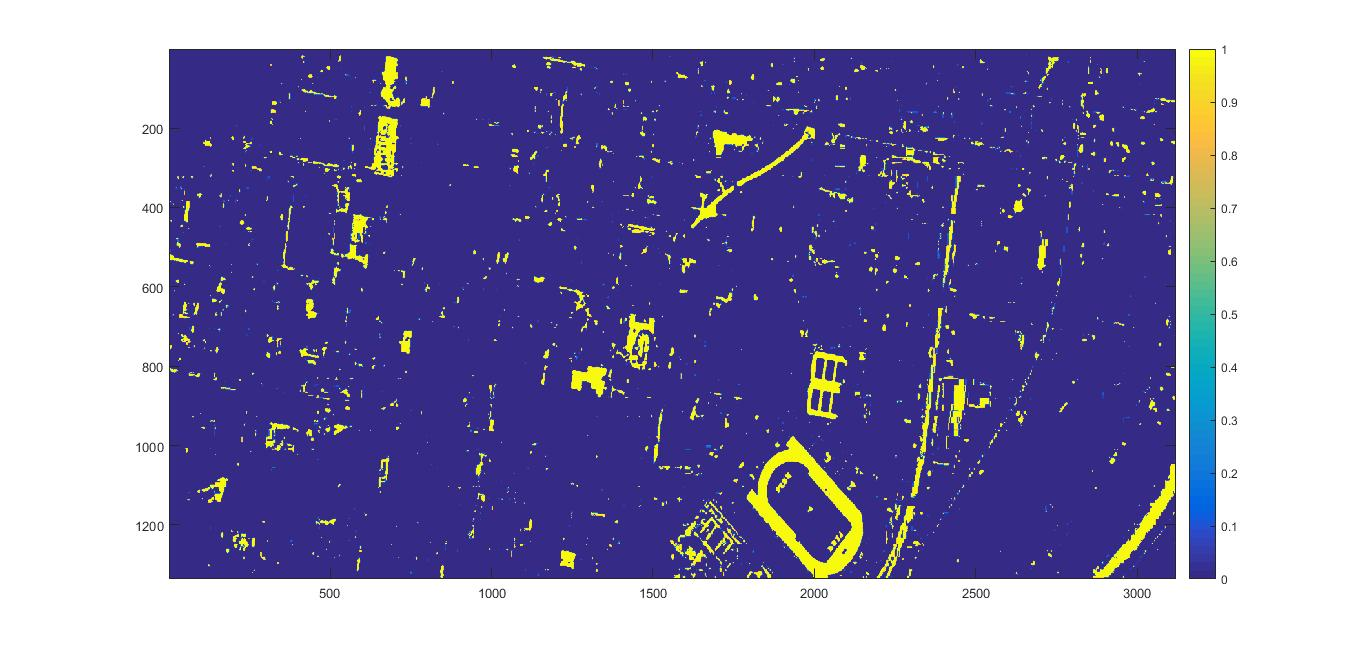
\includegraphics[trim={6cm 2.5cm 4.5cm 1.6cm},clip,scale=0.18]{18.jpg} & \vspace{-3cm} YCbCr, Gaussian Blur, morphological operations \\ 
\bottomrule
\end{tabular} 
\end{table*}

\begin{table*}
\centering
\begin{tabular}{>{\centering\arraybackslash}M{8mm}cc>{\centering\arraybackslash}M{20mm}}
\toprule
Feature & Masked RGB Image & Feature & Post Processing \\ 
\midrule 
\vspace{-3cm}
\hspace{-0.2cm}
Grey roof & 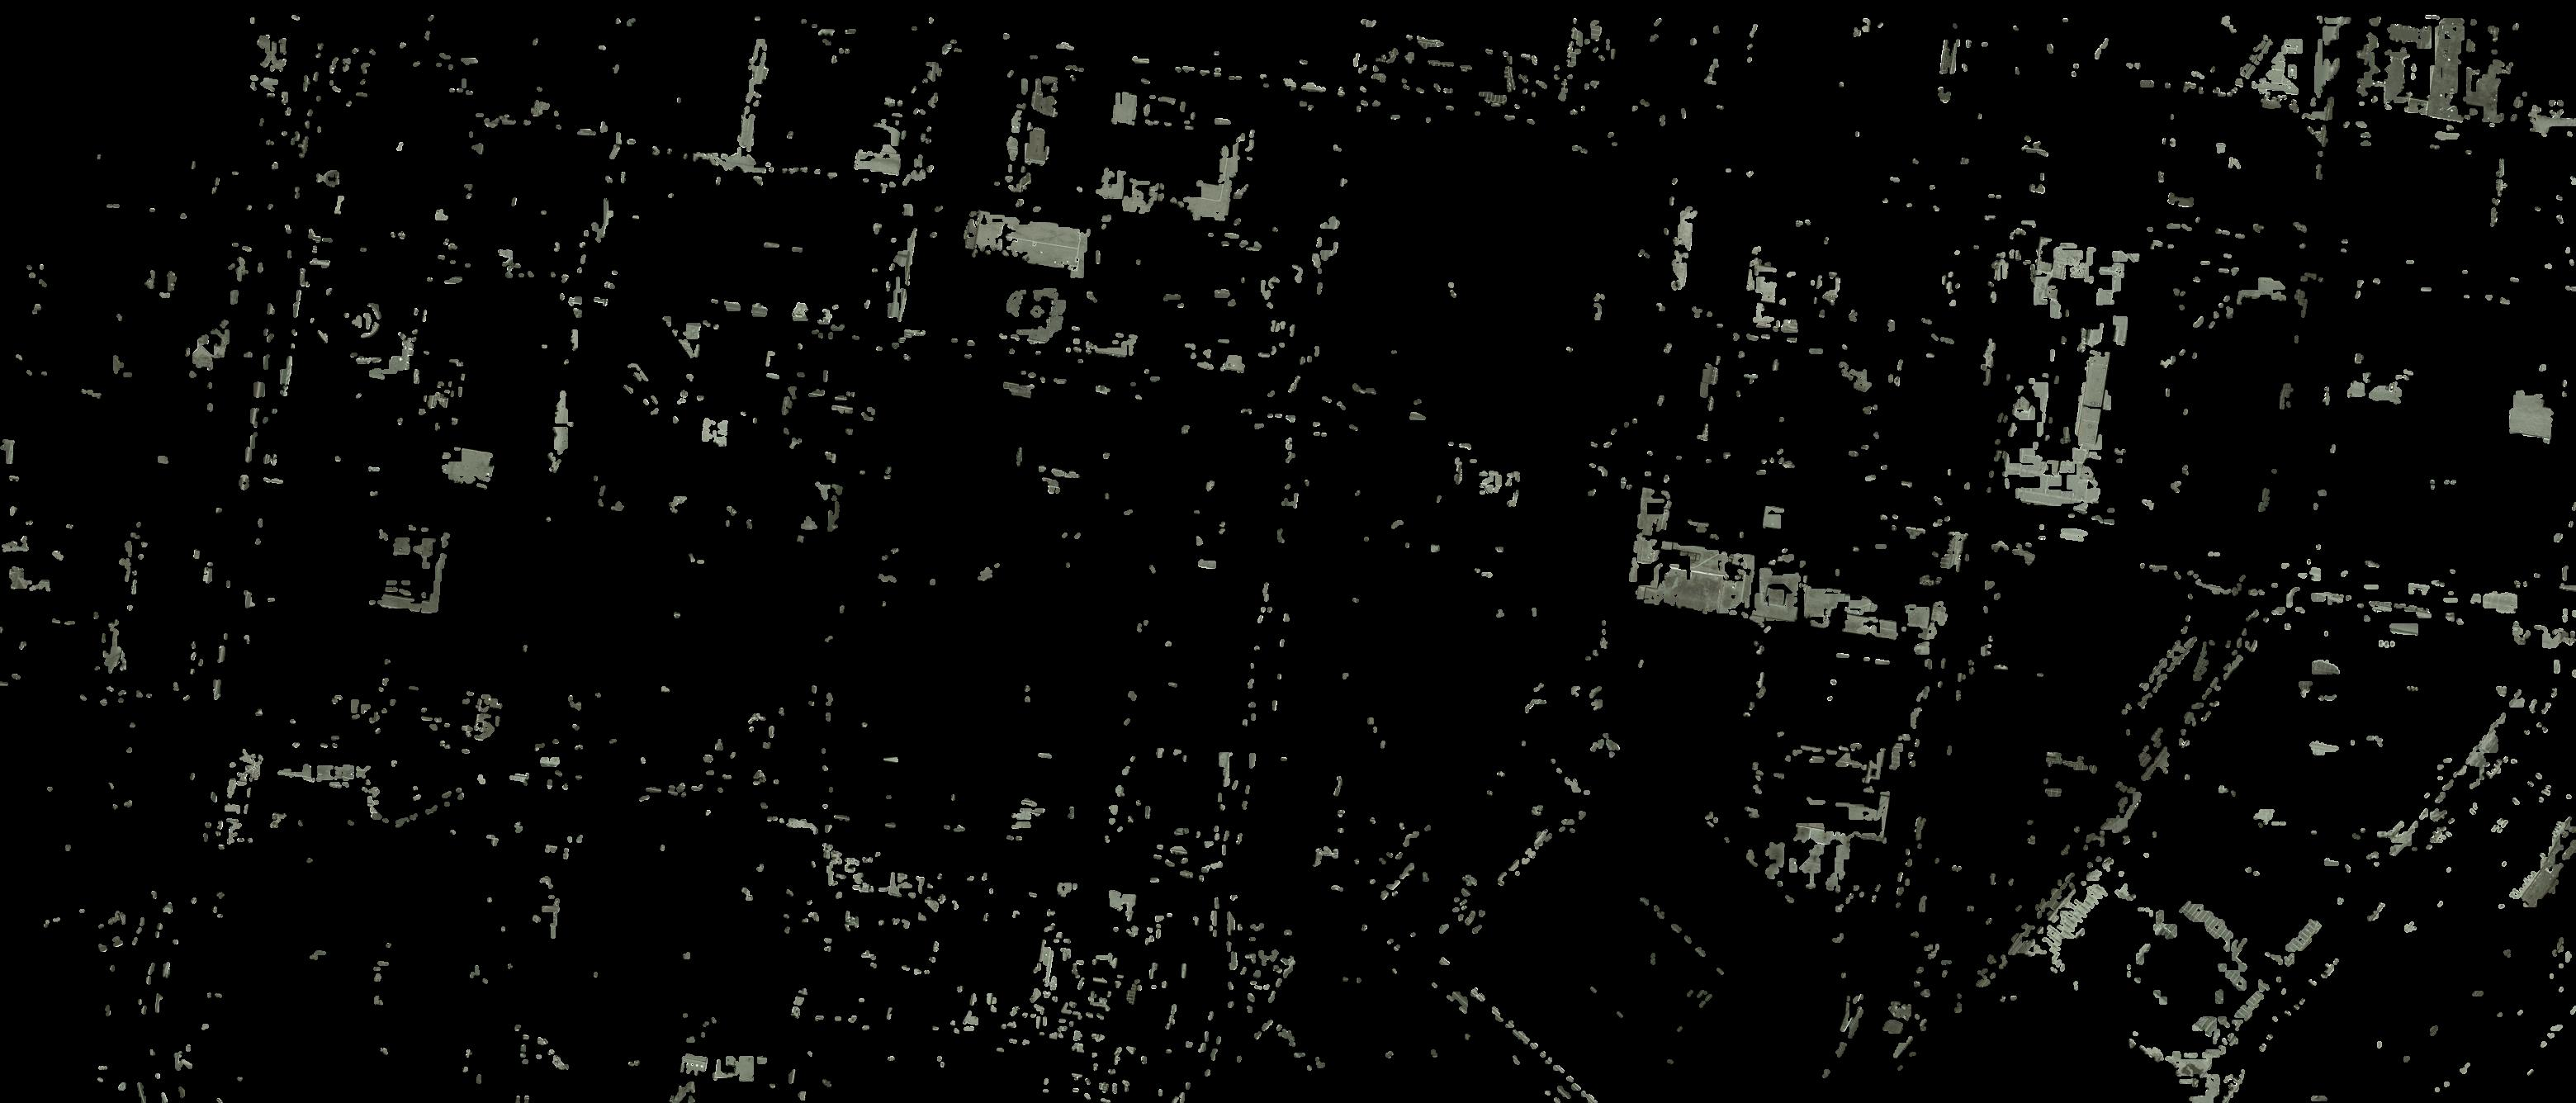
\includegraphics[clip,scale=0.07]{19rgb.jpg} & 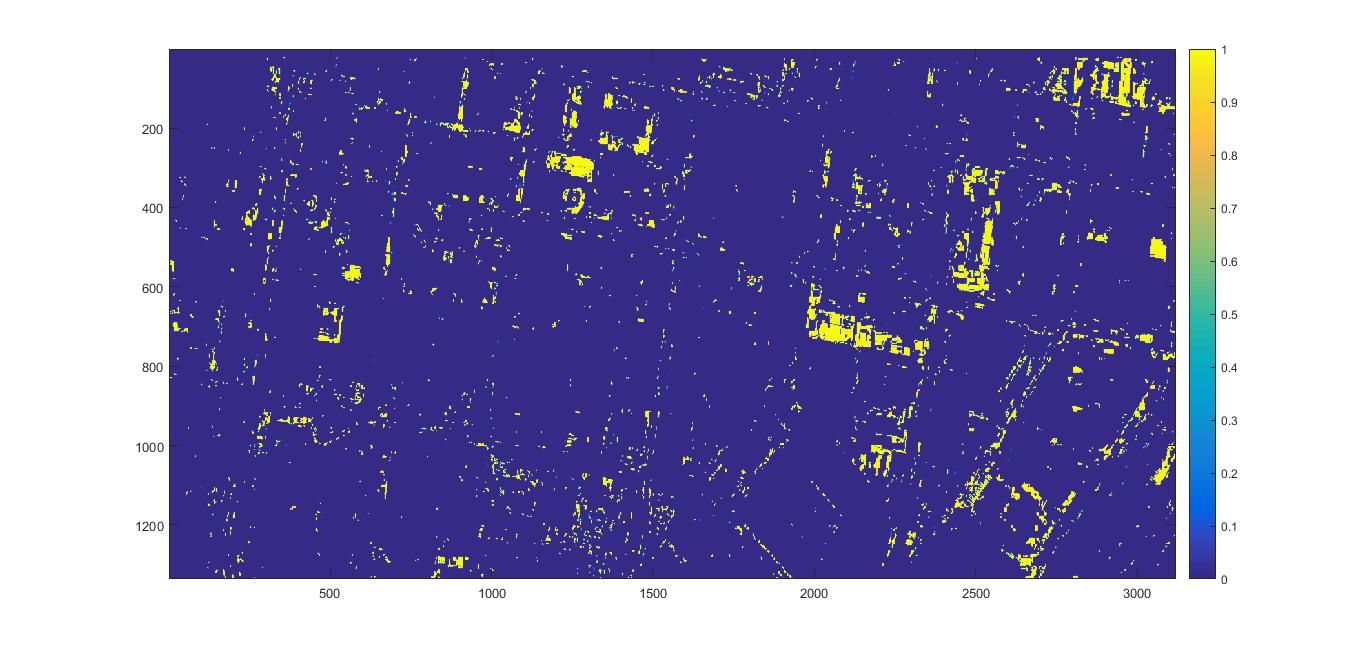
\includegraphics[trim={6cm 2.5cm 4.5cm 1.6cm},clip,scale=0.18]{19.jpg} & \vspace{-3cm}YCbCr, Gaussian Blur, morphological operations, eccentricity \\ 
\midrule 
\vspace{-3cm}
\hspace{-0.4cm}
Green trees & 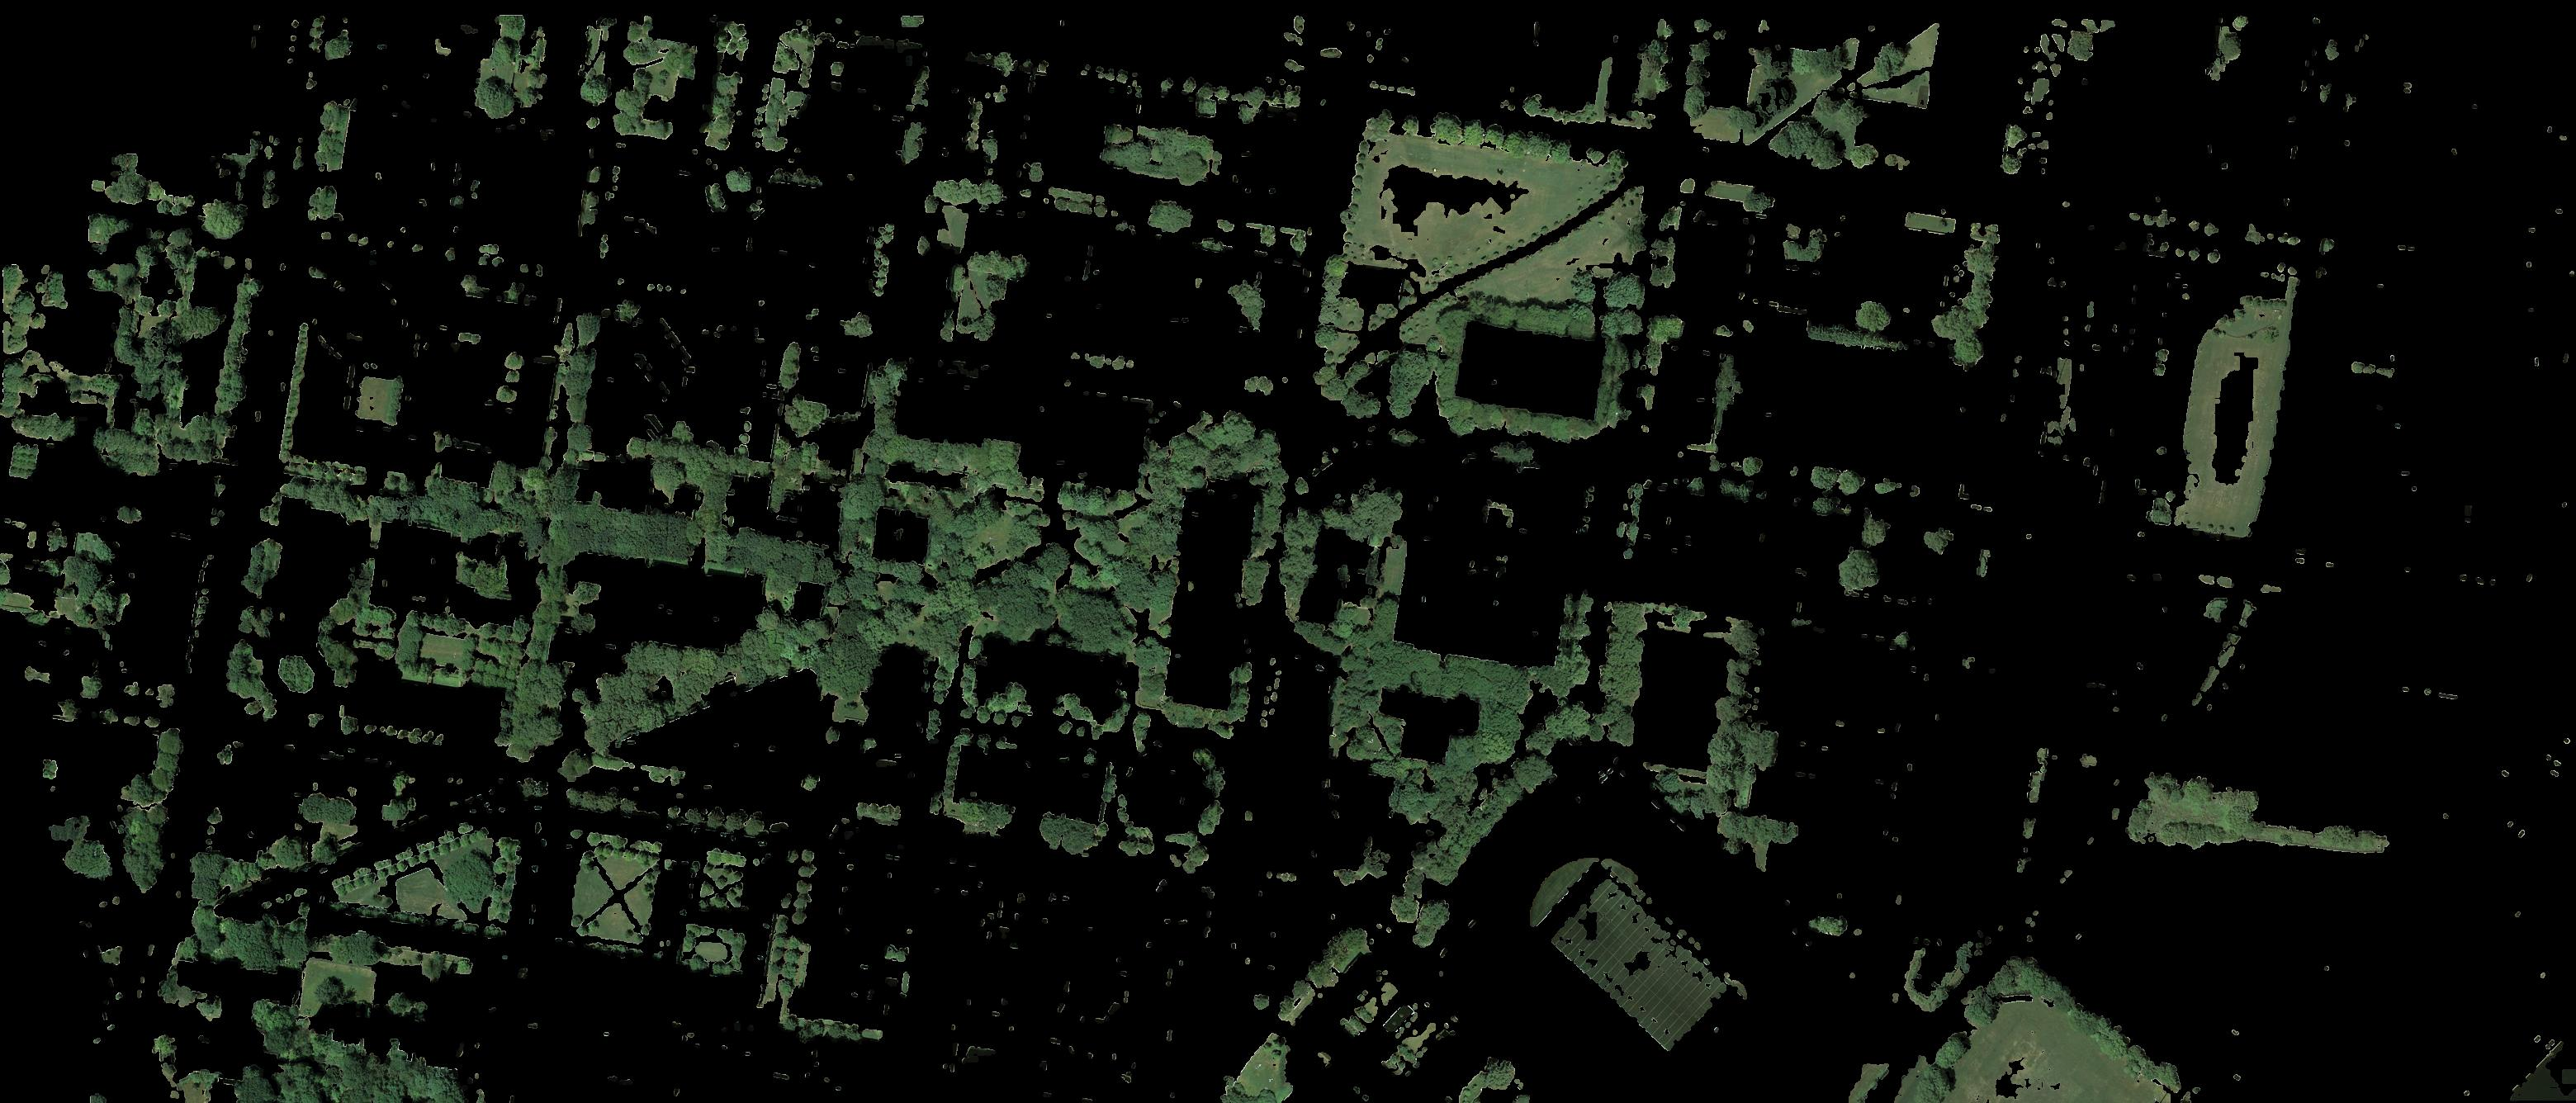
\includegraphics[clip,scale=0.07]{20rgb.jpg} & 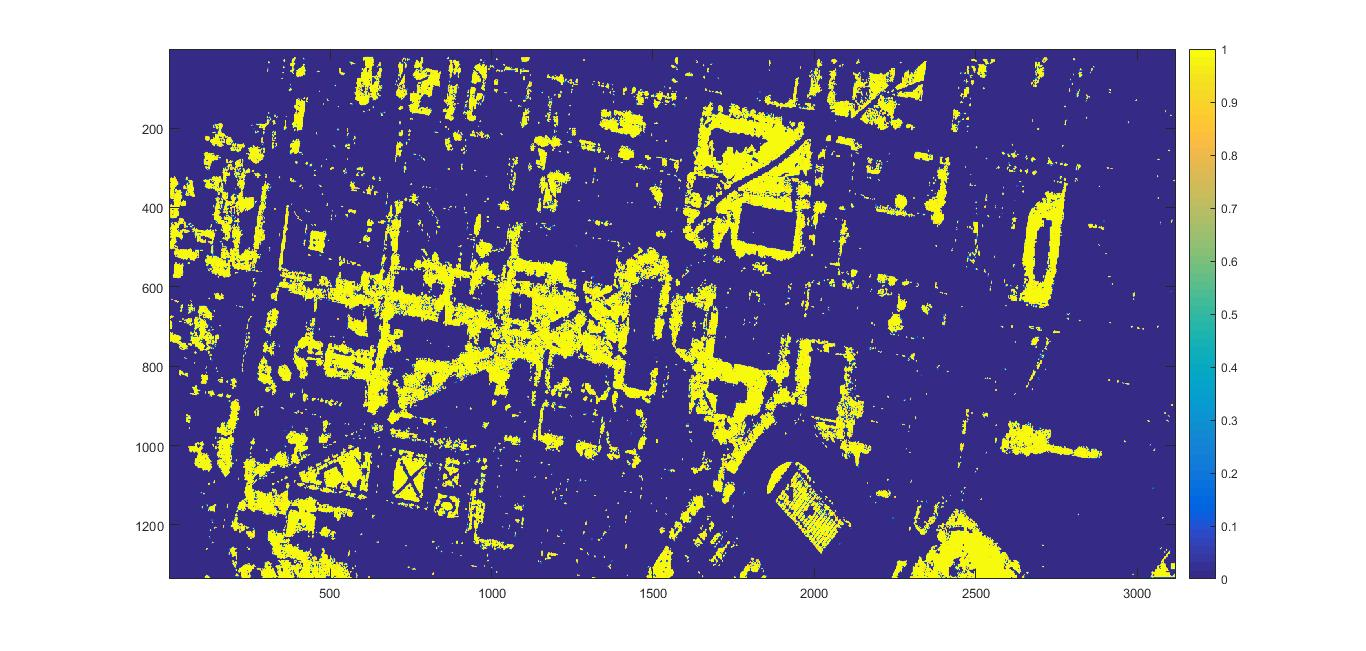
\includegraphics[trim={6cm 2.5cm 4.5cm 1.6cm},clip,scale=0.18]{20.jpg} & \vspace{-3cm}HSV, Gaussian Blur, morphological operations \\ 
\midrule 
\vspace{-3cm}
\hspace{-0.3cm}
Dark Gray roof & 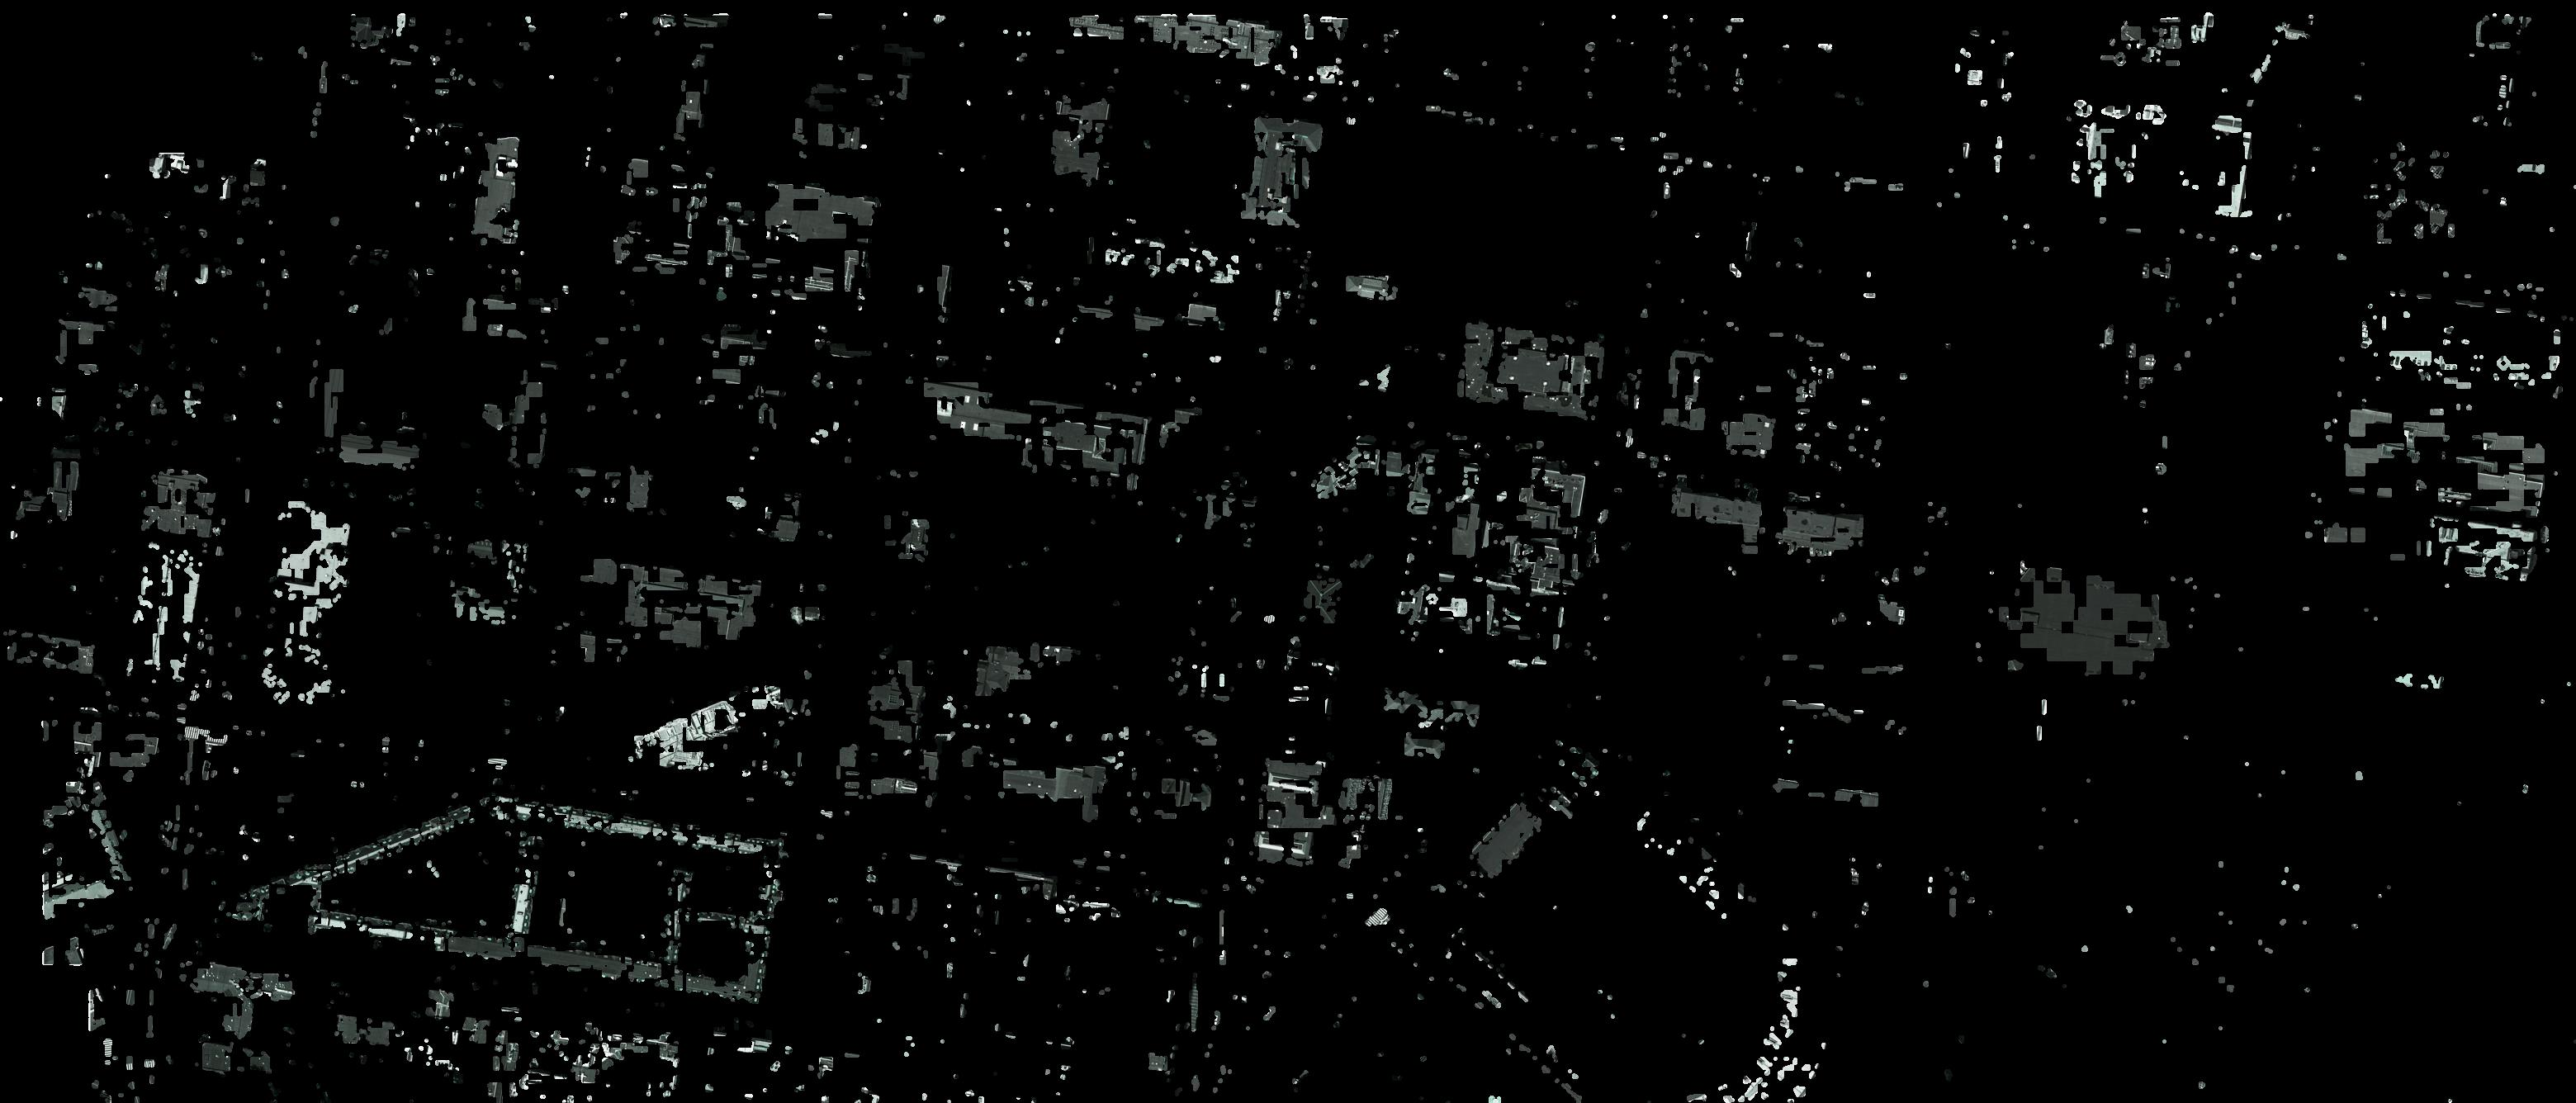
\includegraphics[clip,scale=0.07]{21rgb.jpg} & 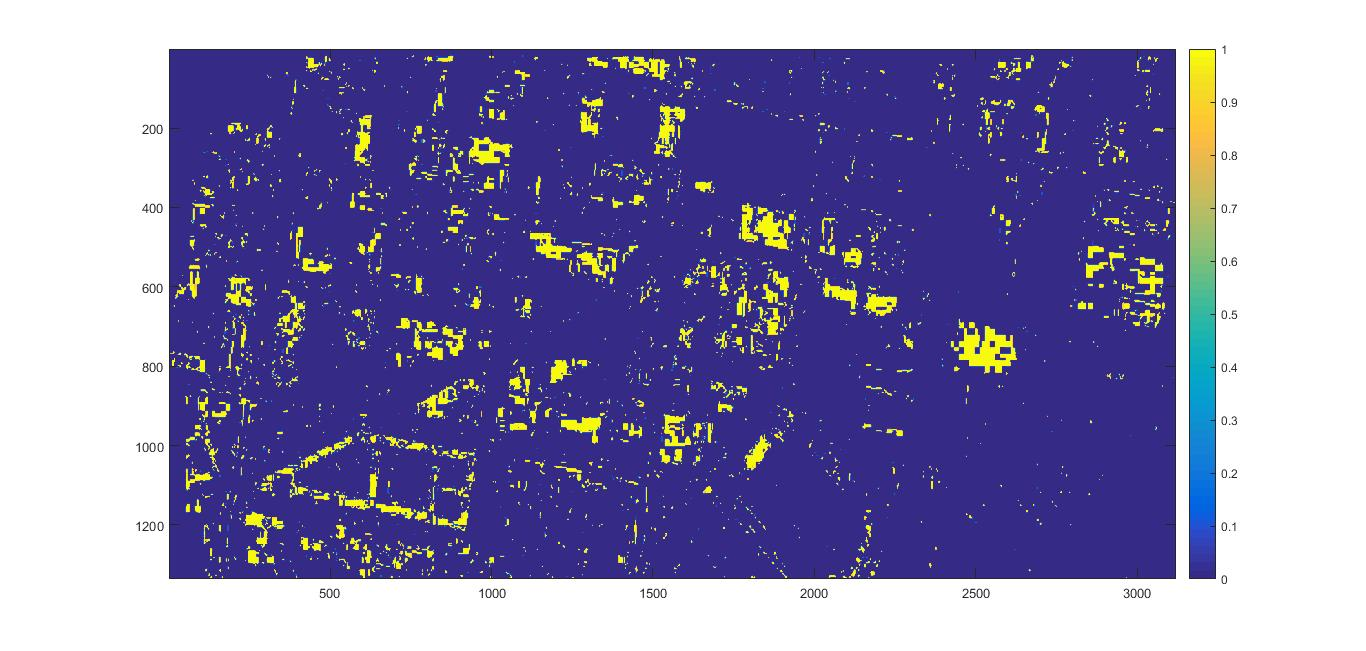
\includegraphics[trim={6cm 2.5cm 4.5cm 1.6cm},clip,scale=0.18]{21.jpg} & \vspace{-3cm}YCbCr, Gaussian Blur, morphological operations, eccentricity \\ 
\midrule 
\vspace{-3cm}
\hspace{-0.4cm}
White roof & 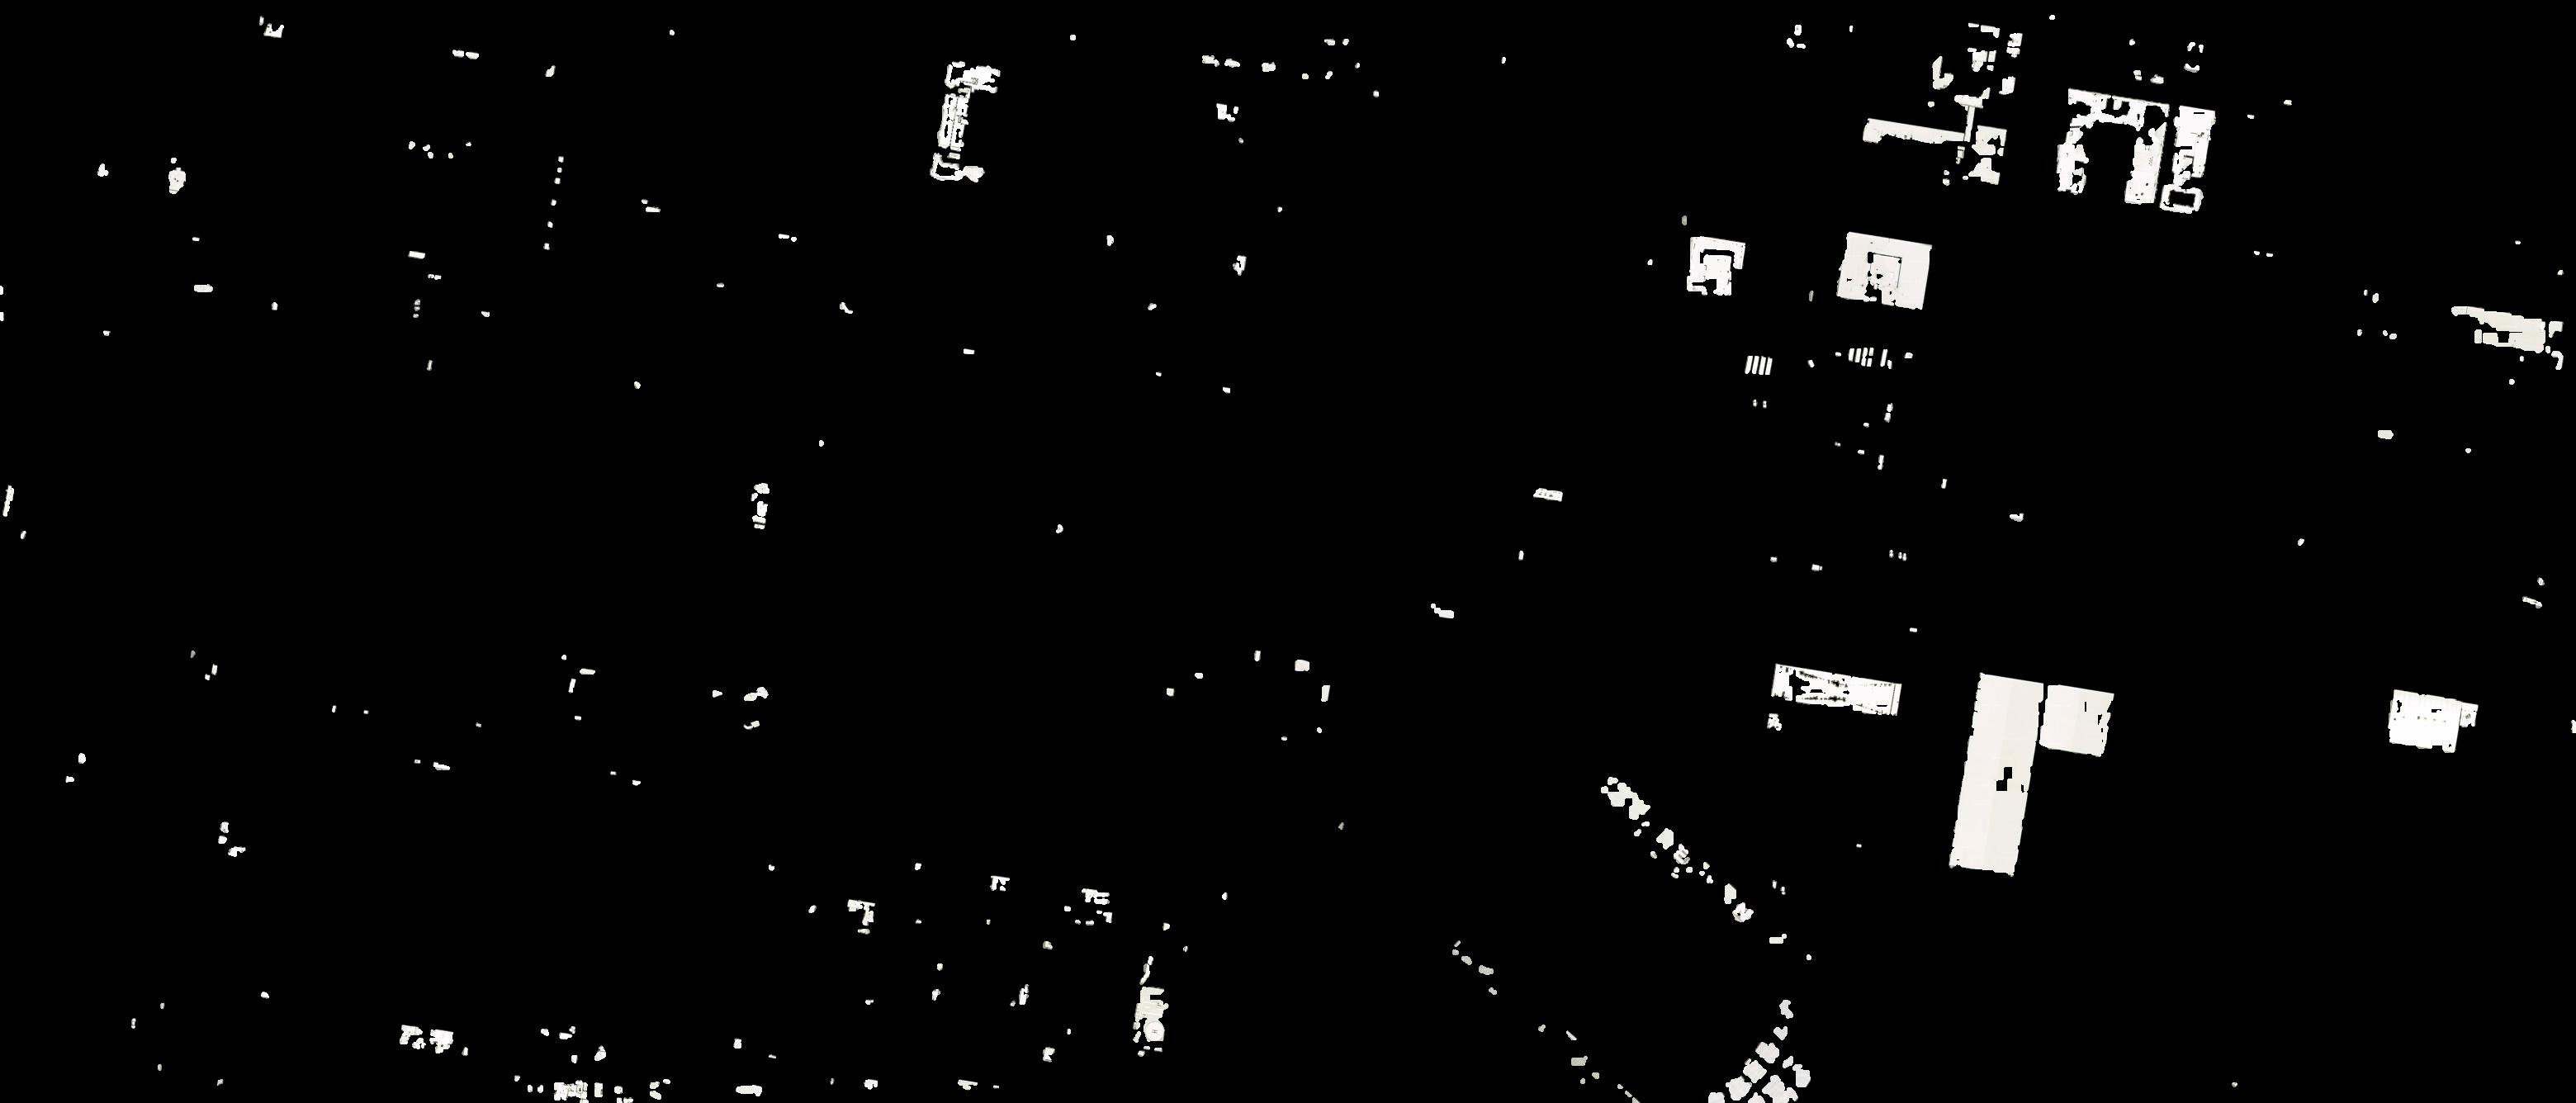
\includegraphics[clip,scale=0.07]{22rgb.jpg} & 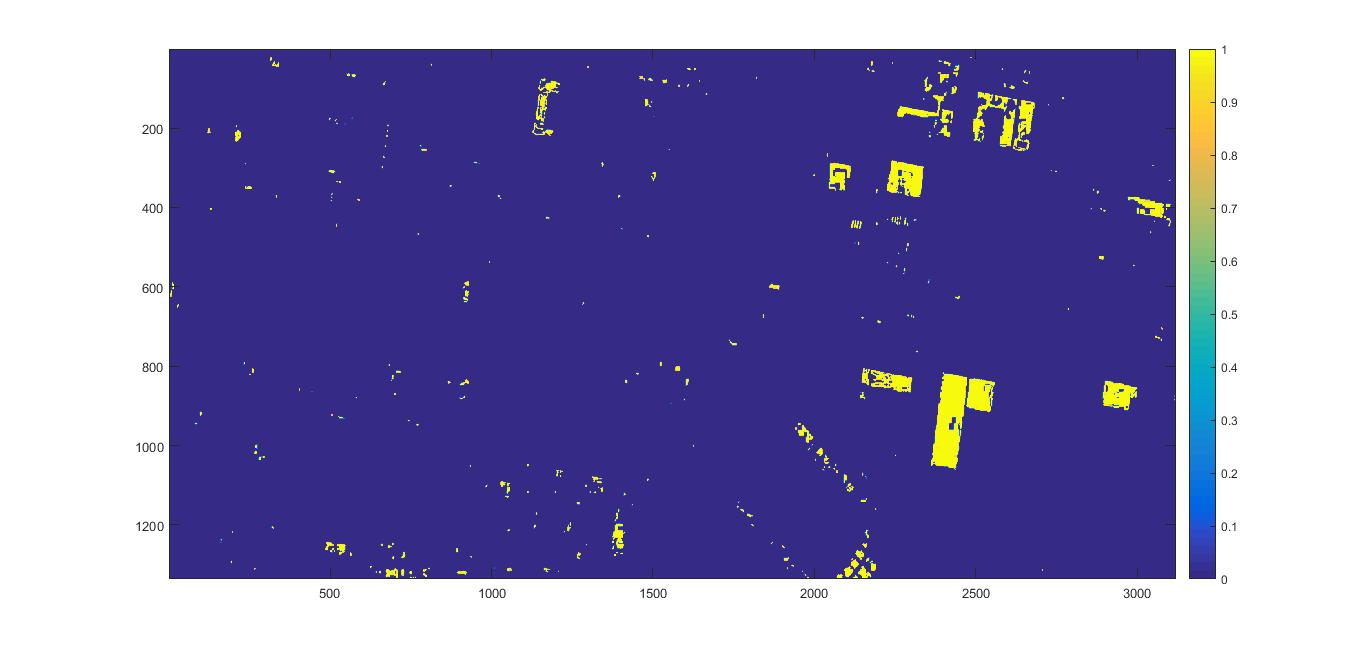
\includegraphics[trim={6cm 2.5cm 4.5cm 1.6cm},clip,scale=0.18]{22.jpg} & \vspace{-3cm}HSV, Gaussian Blur, morphological operations \\  
\midrule 
\vspace{-3cm}
\hspace{-0.4cm}
Cream roof & 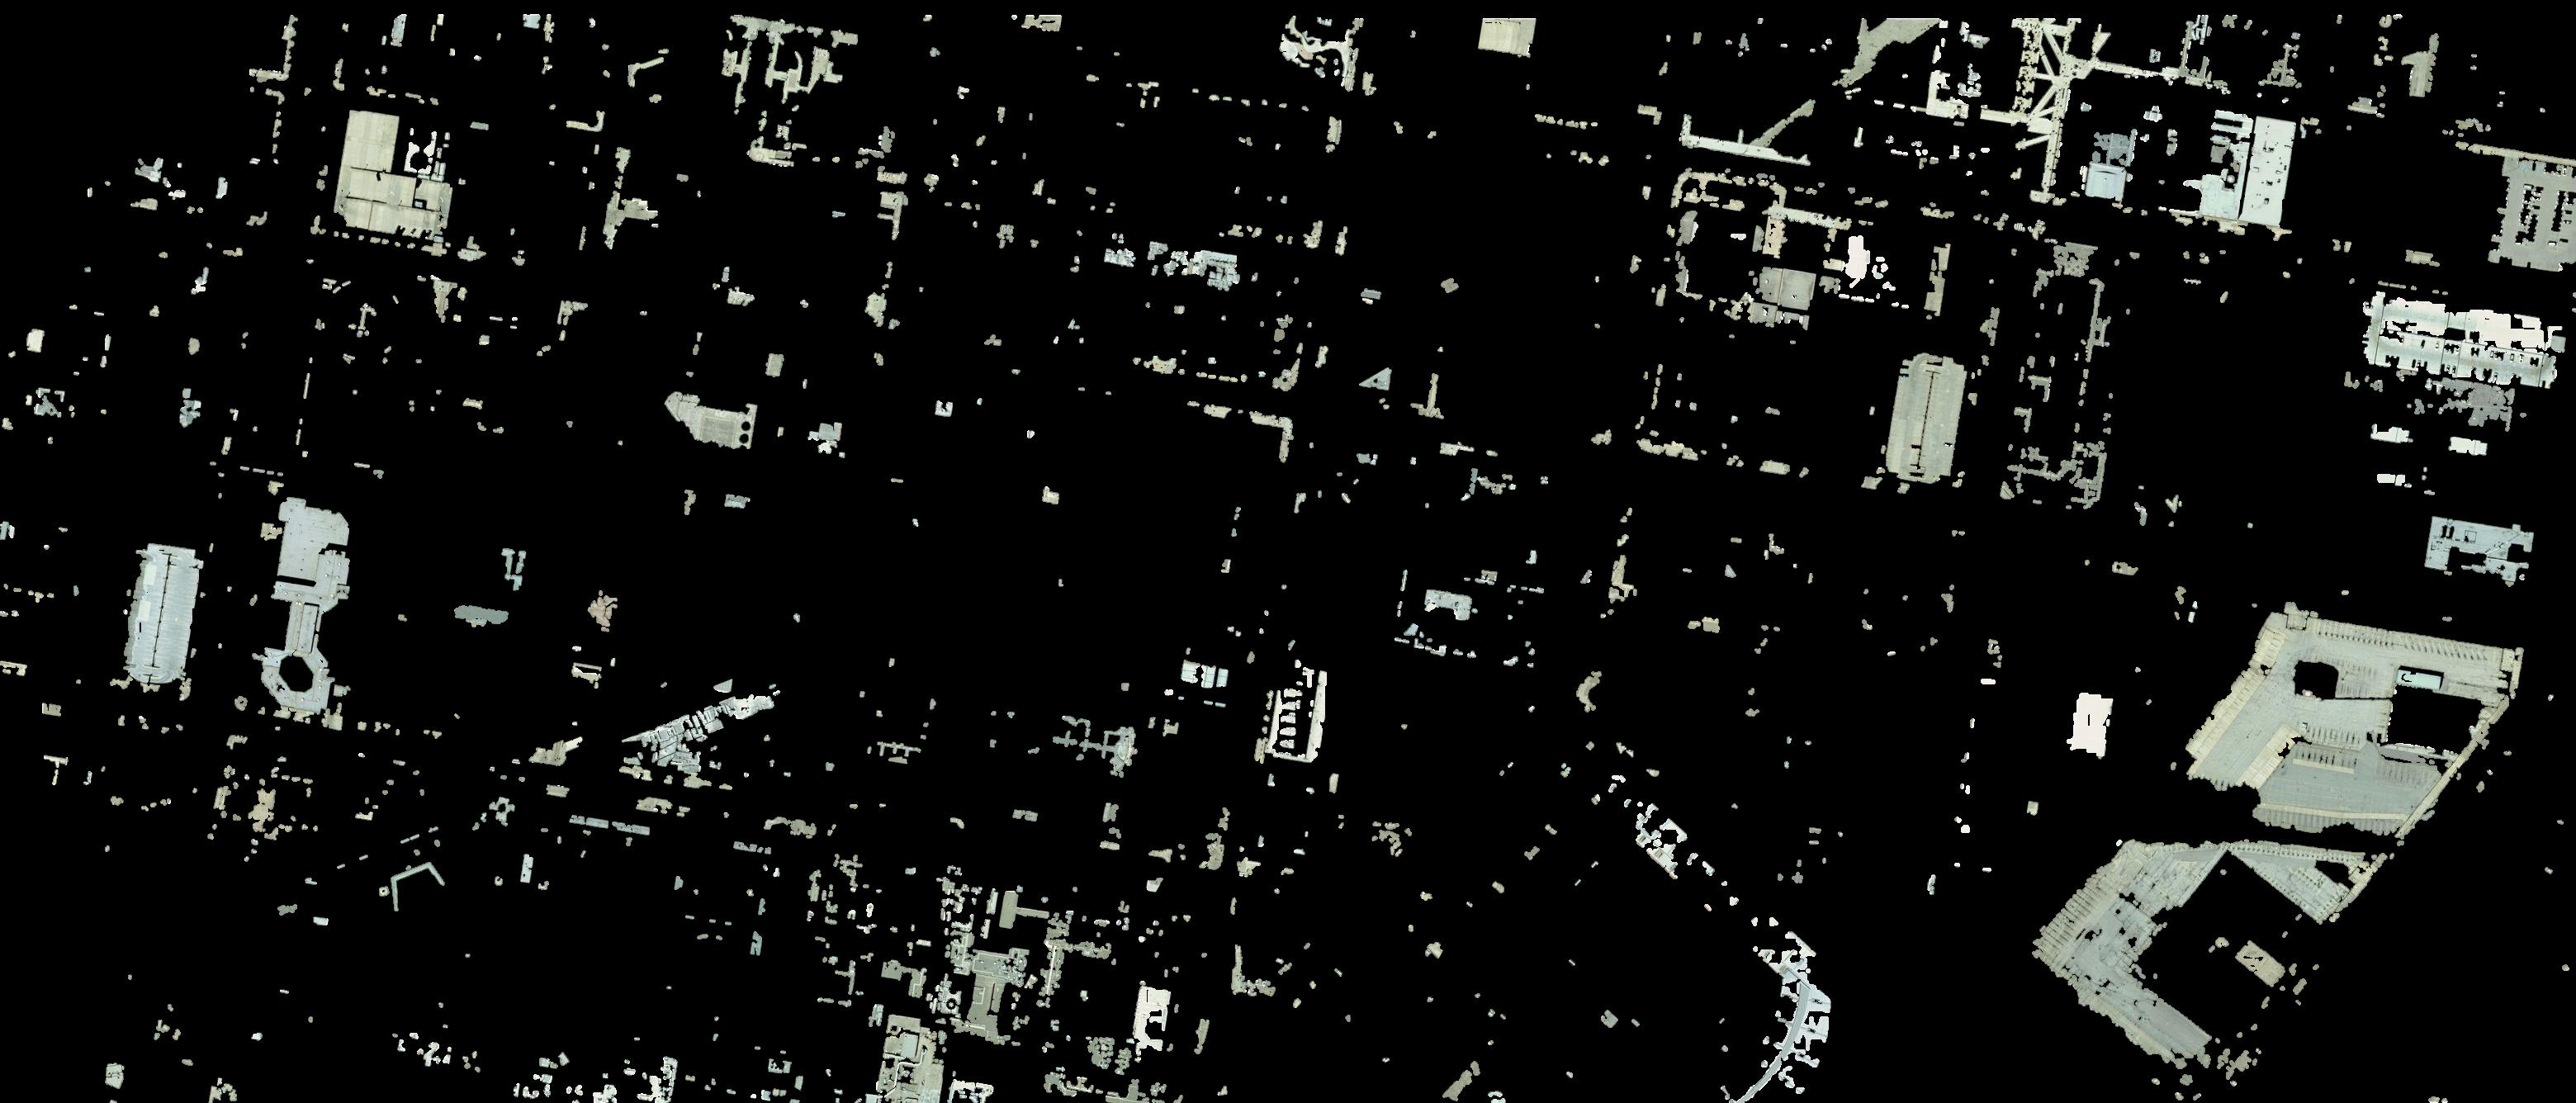
\includegraphics[clip,scale=0.07]{23rgb.jpg} & 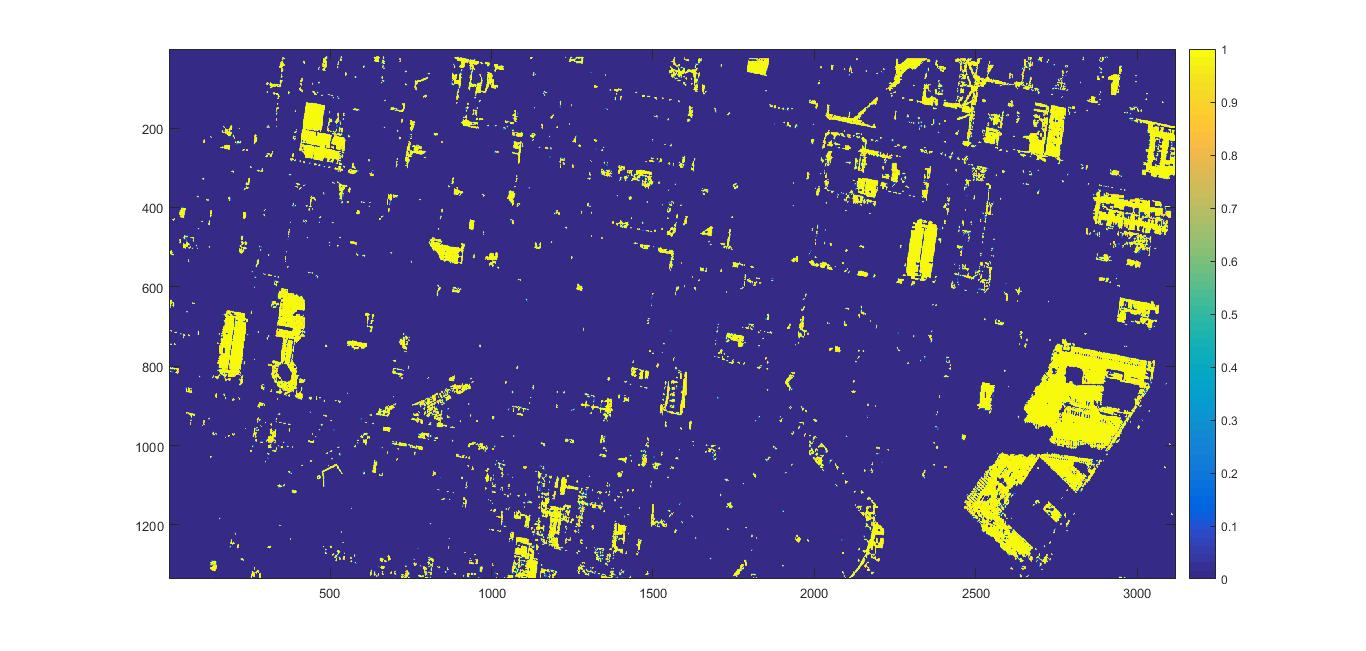
\includegraphics[trim={6cm 2.5cm 4.5cm 1.6cm},clip,scale=0.18]{23.jpg} & \vspace{-3cm}YCbCr, Gaussian Blur, morphological operations \\ 
\midrule 
\vspace{-3cm}
\hspace{-0.6cm}
Roads & 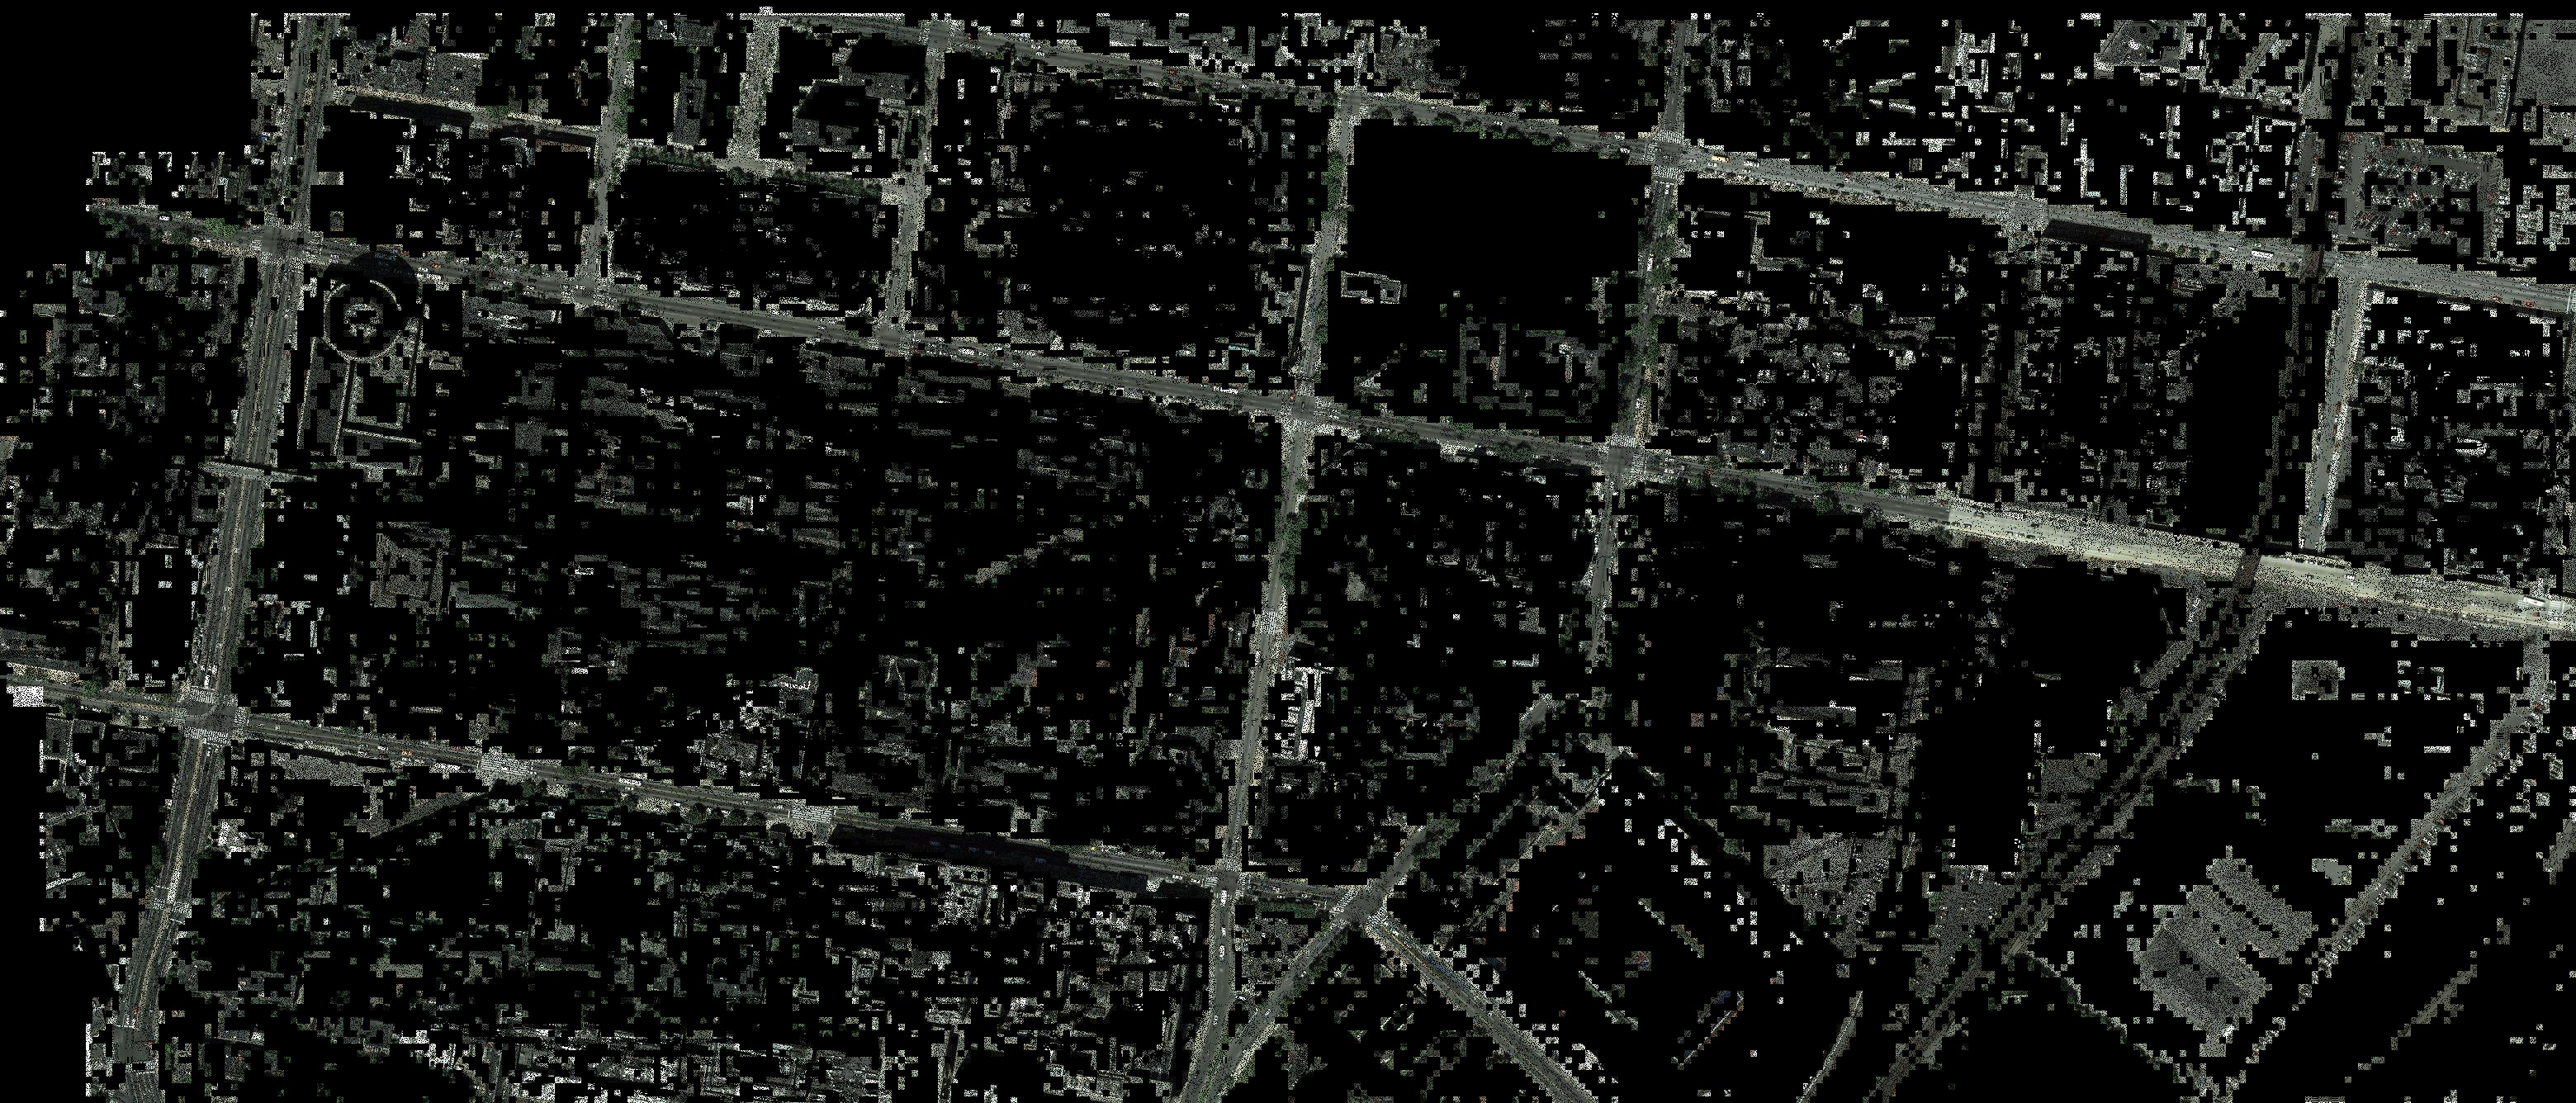
\includegraphics[clip,scale=0.07]{24rgb.jpg} & 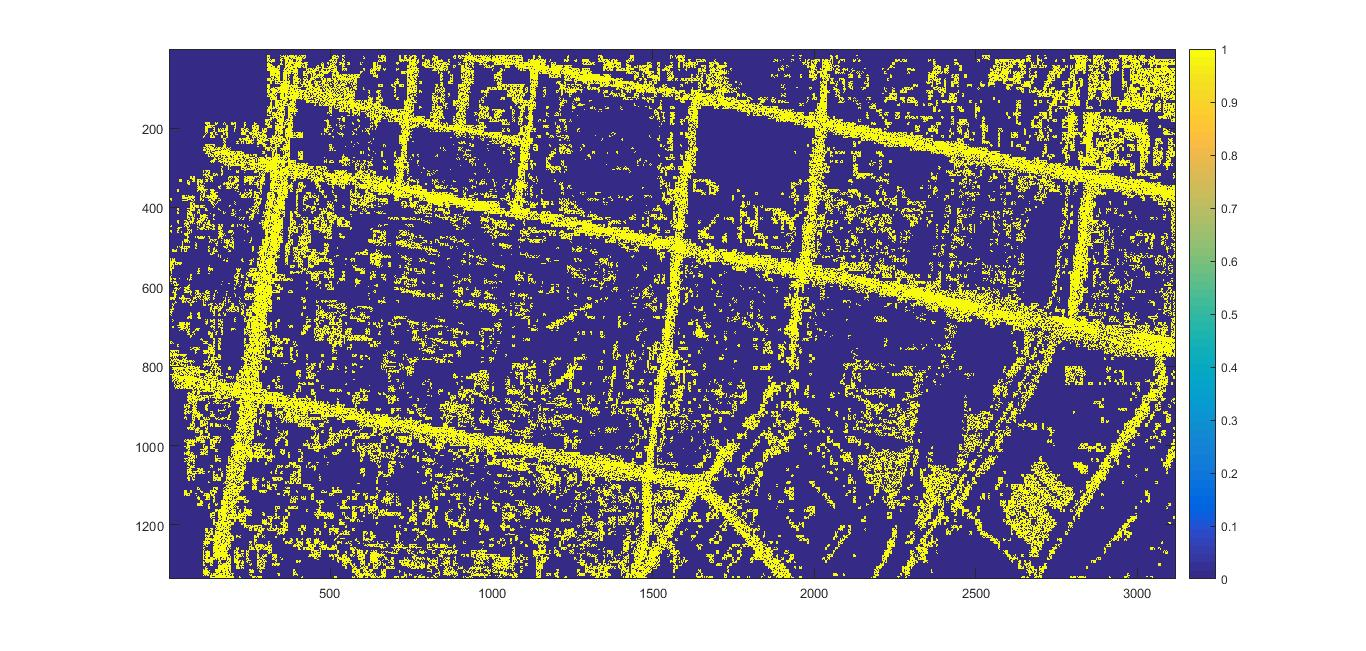
\includegraphics[trim={6cm 2.5cm 4.5cm 1.6cm},clip,scale=0.18]{24.jpg} & \vspace{-3cm}Lab, Gaussian Blur, morphological operations, eccentricity \\ 
\bottomrule
\end{tabular} 
\end{table*}

\begin{figure*}[hbtp]
\caption{Cost map for Driving}
\centering
\includegraphics[scale=0.6]{costs_car.jpg}
\label{fig:costCar}
\end{figure*}

\begin{figure*}[hbtp]
\caption{Cost map for Walking}
\centering
\includegraphics[scale=0.6]{costs_walk.jpg}
\label{fig:costWalk}
\end{figure*}

\begin{figure*}[hbtp]
\caption{Test set results for Driving}
\centering
\includegraphics[scale=0.6]{drive.jpg}
\label{fig:drive}
\end{figure*}

\begin{figure*}[hbtp]
\caption{Test set results for Walking}
\centering
\includegraphics[scale=0.6]{walk.jpg}
\label{fig:walk}
\end{figure*}

%\begin{thebibliography}{9}

%\end{thebibliography}

%----------------------------------------------------------------------------------------
%	REFERENCE LIST
%----------------------------------------------------------------------------------------
%\phantomsection
%\bibliographystyle{unsrt}
%\bibliography{sample}

%---------------------------------------------------------------------------------------- 

\end{document}

%% Convergence graph
%% State transition matrixes
%% Cross validation matrix